%%
%% This is file `sample-sigconf.tex',
%% generated with the docstrip utility.
%%
%% The original source files were:
%%
%% samples.dtx  (with options: `sigconf')
%% 
%% IMPORTANT NOTICE:
%% 
%% For the copyright see the source file.
%% 
%% Any modified versions of this file must be renamed
%% with new filenames distinct from sample-sigconf.tex.
%% 
%% For distribution of the original source see the terms
%% for copying and modification in the file samples.dtx.
%% 
%% This generated file may be distributed as long as the
%% original source files, as listed above, are part of the
%% same distribution. (The sources need not necessarily be
%% in the same archive or directory.)
%%
%% The first command in your LaTeX source must be the \documentclass command.
\documentclass[sigconf, nonacm, natbib, screen, balance=False]{acmart}

% Documentation for packages
% - ACM Article Template
%    https://www.acm.org/publications/proceedings-template
% - Pseudocode typesetting CLRS-style:
%    https://www.cs.dartmouth.edu/~thc/clrscode/clrscode3e.pdf
% - Python code typesetting
%    http://ctan.uib.no/macros/latex/contrib/listings/listings.pdf
% - AMS Math
%    http://ctan.uib.no/macros/latex/required/amsmath/amsldoc.pdf
% - Graphics
%    http://ctan.uib.no/macros/latex/required/graphics/grfguide.pdf

\usepackage{clrscode3e}  
\usepackage{listings}
\lstset{language=Python, basicstyle=\ttfamily}
\usepackage{titlesec}
\usepackage{enumitem}
\usepackage{blindtext}
\usepackage{amsmath}

% based on https://tex.stackexchange.com/questions/279240/float-for-lstlisting
\usepackage{float}
\floatstyle{ruled}
\newfloat{listing}{tbph}{lop}
\floatname{listing}{Listing}
\def\lstfloatautorefname{Listing} % needed for hyperref/auroref

\titleformat*{\subsection}{\Large\bfseries}
\titleformat*{\subsubsection}{\large\bfseries}

\citestyle{acmauthoryear}
\newcommand{\floor}[1]{\left\lfloor #1 \right\rfloor}

%% end of the preamble, start of the body of the document source.
\begin{document}

%%
%% The "title" command has an optional parameter,
%% allowing the author to define a "short title" to be used in page headers.
\title{Benchmarking sorting algorithms in Python}
\subtitle{INF221 Term Paper, NMBU, Autumn 2020}

\author{Mohamed Radwan}
\email{mohamed.radwan@nmbu.no}
\affiliation{}  % separates Jane's and Joe's author block
\author{Nasibeh Mohammadi}
\email{nasibeh.mohammadi@nmbu.no}

%% The abstract is a short summary of the work to be presented in the
%% article.
\begin{abstract}
The objective of this paper is to show the results of performing benchmark experiments on sorting algorithms. We implemented several sorting algorithms and compared them in terms of their run-time. The algorithms were investigated into four categories: quadratic (Insertion-Sort and Bubble-Sort), sub-quadratic (Merge-Sort and Quick-Sort), combined Merge-Insertion-Sort and built-in (Python-Sort and Numpy-Sort) algorithms. The input data were lists of float values with sizes from $2^{4}$ to $2^{14}$ in the form of $3$ different ordering permutations: sorted, reversed and random ordering. The study was conducted using Python programming language and several libraries like Numpy, Scipy, Pandas and Matplotlib. Quick-Sort showed very similar run-time in sorting reversed and sorted data. Merge-Sort also showed the same observation. For finding an explanation for these behaviours, we investigated these observations further by measuring the number of comparisons that Merge-Sort and Quick-Sort executed in sorting the data. The study also shows that Numpy-Sort and Python-Sort are faster than all other implemented algorithms. Bubble-Sort is the slowest sorting algorithm among all these algorithms. Additionally, we implemented a combined Merge-Insertion-Sort which performed slightly faster than Merge-Sort. A challenging question is left open that is why Python-Sort is $10$ times faster than our implementation of Merge-Insertion-Sort. 
\end{abstract}
%%
%% This command processes the author and affiliation and title
%% information and builds the first part of the formatted document.
\maketitle
\section{Introduction}\label{sec:intro}
Sorting algorithms play an essential role in implementing and optimizing efficient algorithms that solve our problems. In this study, we aimed to examine whether the sorting algorithms follow the theoretical run-time. We wanted to compare the theory with real performance of the algorithms and explain the results. Theoretical details about each type of sorting algorithms are explained in the "Theory" section where we give description on the theoretical expectations of the algorithms' execution times. In third section, "Methods", we explain the methods utilised in this research for executing the benchmarks and the hardware and software specifications. In the "Result" section, the numerical results and observations are explained in details supported by figures. In the "Discussion" section, we use our findings and combine our observed results with the theoretical expectations to understand the behaviours of these sorting algorithms. 

\section{Theory}\label{sec:theory}

\subsection{Quadratic Algorithms}
Insertion-Sort and Bubble-Sort belong to this family of sorting algorithms where the run-time follows a quadratic big theta time complexity $\Theta(n^2)$.  

\subsubsection{Insertion-Sort}\label{sec:insertion_sort}
\hfill\\
According to \citet{CLRS_2009}, "Insertion-Sort is an efficient algorithm for sorting a small number of elements". Insertion-Sort does the sorting of the input data in-place. This algorithm, as shown in the pseudo-code in listing~\ref{lst:insertion_sort}, starts by taking one non-sorted element at a time and compares it with already sorted elements and inserts it in correct place among sorted elements. Comparison is done in a way that if the element is smaller than the preceding element, they will be swapped. These swaps are done following inner condition, as shown in listing~\ref{lst:insertion_sort}, which is repeated until $j$ reaches $-1$ (each time the while loop is performed, $j$ is decremented by $1$). Those swaps are executed until all elements before and including the element at index $i$ are in sorted order. This process is repeated until all the elements are in sorted order. 
\hfill\\
This algorithm at worst and average cases will go through the two loops, so the worst and average case scenario of Insertion-Sort follow the quadratic form as shown in equation~\ref{eq:insertion_sort}.
\begin{equation}
  T(n) = \Theta(n^2) \; \label{eq:insertion_sort}
\end{equation}
Insertion-Sort, in the best case scenario, has a linear run-time of $\Theta(n)$ where the data are already sorted and the condition of while-loop in line 4 in the algorithm is not satisfied.

\begin{listing}
  % Pseudocode caption above the code.
  \caption{Insertion-Sort algorithm pseudo-code (modified after from \citet[Ch.~2.1]{CLRS_2009}).}
  \label{lst:insertion_sort}
  %
  % For documentation on how to typeset CLRS-style pseudocode, see
  % https://www.cs.dartmouth.edu/~thc/clrscode/clrscode3e.pdf
  %
  \begin{codebox}
    \Procname{$\proc{Insertion-Sort}(A)$}
    \li \For $i \gets 2 \To \attrib{A}{length}$ 
    \Do
    \li $Key \gets A[i]$
    \li $j \gets  i-1$
    \li \While $j > 0$ and $key < A[j]$
    \Do
    \li $A[j+1] \gets A[j] $
    \li $j \gets j-1$
    \End
    \li $A[j+1] = key$
    \End
  \end{codebox}
\end{listing}

\subsubsection{Bubble-Sort}\label{sec:bubble_sort}
\hfill\\
According to \citet{CLRS_2009}, Bubble-Sort is in-place sorting algorithm. The algorithm, as shown in listing~\ref{lst:bubble_sort}, works from the leftmost element and goes to the rightmost and swaps the pairs which are not sorted. It swaps every pairs of elements if the condition in line $3$ of the algorithm in the listing~\ref{lst:bubble_sort} is satisfied. In the first run, the algorithm iterates through all elements and pushes the greatest element to the rightmost place. In the second run, the algorithm iterates over all elements except the last element and swaps pairs of elements. These iterations are repeated until $i$ reaches the end of the array.
\hfill\\
The algorithm contains one nested loop thus the run-time is as shown in the equation~\ref{eq:bubble_sort}. The study made by \citet{astrachan} shows that Bubble-Sort, in general, is $3$ times slower than Insertion-Sort.
\begin{equation}
  T(n) = \Theta(n^2) \;   \label{eq:bubble_sort}
\end{equation}
\begin{listing}
  % Pseudocode caption above the code.
  \caption{Bubble-Sort algorithm pseudo-code (modified after \citet[Ch.~2.3]{CLRS_2009}).}
  \label{lst:bubble_sort}
  %
  % For documentation on how to typeset CLRS-style pseudocode, see
  % https://www.cs.dartmouth.edu/~thc/clrscode/clrscode3e.pdf
  %
  \begin{codebox}
    \Procname{$\proc{Bubble-Sort}(A)$}
    \li \For $i \gets 1 \to \attrib{A}{length}$
    \Do
    \li \For $j \gets 1 \to \attrib{A}{length}-1$
    \Do
    \li \If $A[j]$ > $A[j+1]$
    \li \Then exchange $A[j]$ with $A[j+1]$
    \End
    \End
  \end{codebox}
\end{listing}
\hfill\\
\subsection{Sub-Quadratic Algorithms}
This family of algorithms contains Quick-Sort and Merge-Sort. Those algorithms follow a logarithmic run-time $\Theta(n \cdot \lg n)$. These algorithms use the divide-and-conquer approach where the problem is broken into sub-problems that are solved recursively and the solutions are combined to form a solution to the original problem.
\subsubsection{Quick-Sort}\label{sec:quick_sort}
\hfill\\
According to \citet{CLRS_2009}, Quick-Sort algorithm is in-place algorithm that follows divide and conquer approach where it splits the data into two partitions based on the pivot. Elements in the left partition are smaller than the pivot and elements in the right partition are larger than the pivot. Recursive calls will be done on left and right sub-arrays till all arrays are sorted. Pseudo-code of the Quick-Sort algorithm is shown in listing~\ref{lst:quick_sort}. Assuming that partitioning is done in the median of the data, time complexity for the algorithm is as shown in equation~\ref{eq:quick_best}. 
\begin{equation}
  T(n) = \Theta(n\cdot\lg n) \;.  \label{eq:quick_best} 
\end{equation}
The equation~\ref{eq:quick_best} gives the best case run-time of the algorithm where the pivot is the median. If the pivot is at the beginning of the data, that would result into uneven split and that is a big challenge in terms of run-time. In case of an already sorted data, all non-pivot elements will end up in right sub-array which gives run-time as in the equation~\ref{eq:quick_worst}.
\begin{equation}
  T(n) = \Theta(n^2) \;.  \label{eq:quick_worst}
\end{equation}
Both Quick-Sort and Merge-Sort follow the logarithmic run-time average case. However, \citet{skienna08} stated that properly implemented Quick-Sort is typically $2-3$ times faster than Merge-Sort or Heap-Sort. This claim was supported by the study conducted by \citet{Rajput2012PerformanceCO}.

\begin{listing}
  % Pseudocode caption above the code.
  \caption{Quick-Sort algorithm pseudo-code (modified after from \citet[Ch.~2.1]{CLRS_2009}).}
  \label{lst:quick_sort}
  %
  % For documentation on how to typeset CLRS-style pseudocode, see
  % https://www.cs.dartmouth.edu/~thc/clrscode/clrscode3e.pdf
  %
  \begin{codebox}
  \Procname{$\proc{Quick-Sort}(A)$}
  \li \If $\attrib{A}{length} > 1$
  \li \Then
  $p \gets A[\floor{\attrib{A}{length}/2}]$
  \li \For $i \gets 1 \To \attrib{A}{length}$
  \li \Do
  \If $A[i]$ < $p$
  \li \Then
  $\attrib{l}{insert(A[i])}$
  \li \ElseIf
  $A[i]$ = $p$
  \li \Then
  $\attrib{e}{insert(A[i])}$
  \li \ElseIf
  $A[i]$ > $p$
  \li \Then
  $\attrib{r}{insert(A[i])}$
  \End
  \End
  \li $A \gets \proc{Quick-Sort}(l)+e+\proc{Quick-Sort}(r)$
  \End
  \end{codebox}
\end{listing}

\subsubsection{Merge-Sort}\label{sec:merge_sort}
\hfill\\
Merge-Sort divides $n$ elements sequence, where $n$ is greater than $1$, into two sub-sequences and sort the sub-sequences recursively. Then, it combines the two sorted sub-sequences using the merge function. Pseudo-code for the Merge-Sort algorithm is shown in listing~\ref{lst:merge_sort}. According to \citet[Ch.~2.3]{CLRS_2009}, time complexity for all the cases (best, worst, average) is shown in the equation~\ref{eq:merge_sort}. 
\begin{equation}
  T(n) = \Theta(n \cdot \lg n) \;.  \label{eq:merge_sort}
\end{equation}

\begin{listing}
  % Pseudocode caption above the code.
  \caption{Merge-Sort algorithm pseudo-code (modified after \citet[Ch.~2.3]{CLRS_2009}). The parameter $S$ in the merge function is the start index of the left array to be sorted.}
  \label{lst:merge_sort}
  %
  % For documentation on how to typeset CLRS-style pseudocode, see
  % https://www.cs.dartmouth.edu/~thc/clrscode/clrscode3e.pdf
  %
  \begin{codebox}
  \Procname{$\proc{Merge-Sort}(A)$}
  \li $r =\attrib{A}{Length}$
  \li $p = 1$
  \li \If $r > p$
  \li
  \Then
  $q \gets \floor{(p + r) / 2}$
  \li
  $\proc{Merge-Sort}(A[p \ldots q])$
  \li
  $\proc{Merge-Sort}(A[{q+1} \ldots r])$
  \li
  $\proc{Merge}(A, A[p \ldots q], A[{q+1} \ldots r], 0)$
  \End
  \li \Return A
  \end{codebox}
  \begin{codebox}
  \Procname{$\proc{Merge}(A, L, R, S)$}
  \li $i=1$
  \li $j=1$
  \li $k=S$
  \li \While $i \leq \attrib{L}{Length}$ and $j \leq \attrib{R}{Length}$
  \li \Do
  \If $L[i]$ < $R[j]$
  \li \Then $A[k] \gets L[i]$
  \li $i=i+1$
  \li \Else $A[k]=R[j]$
  \li $j \gets j+1$
  \End
  \li $k=k+1$
  \End
  \li \While $i \leq \attrib{L}{Length}$
  \li \Do
  $A[k] \gets L[i]$
  \li $i=i+1$
  \li $k=k+1$
  \End
  \li \While $j \leq \attrib{R}{Length}$
  \li \Do
  $A[k] \gets R[j]$
  \li $j=j+1$
  \li $k=k+1$ 
  \End
  \end{codebox}
\end{listing}

\subsection{Combined Sort}
We combined the Merge-Sort with Binary-Insertion-Sort as shown in the listing~\ref{lst:combined_sort}. As stated above, Insertion-Sort follows $\Theta (n^2)$ run-time at worst and average cases and $\Theta (n)$ at the best case. Merge-sort follows $\Theta (n \cdot \lg n)$ run-time in all cases. According to \citet{CLRS_2009}, Merge-Sort is generally faster than Insertion-Sort. For the mathematical proof, see \citet[Ch.~2.3]{CLRS_2009}. On the other hand, Insertion-Sort typically runs faster than Merge-Sort for small input sizes. According to \citet{CLRS_2009}, "there will always be a crossover point beyond which Merge-Sort is faster".
\hfill\\
The proposed algorithm is a modified implementation of the \citet{cpythonsourcecode} implementation of Tim-Sort. The algorithm, shown in listing~\ref{lst:combined_sort}, consists of two steps. The first step is dividing the data into 'runs' and applying the Binary-Insertion-Sort (\citet{DBLP:conf/soda/McIlroy93}) on each run. This step is used to sort each run in-place by providing the start and end of each run in the passed parameters to the Binary-Insertion-Sort. The second step uses the merge function that we built earlier in the listing~\ref{lst:merge_sort} to merge the sorted runs. 
\hfill\\
\citet{cpythonsourcecode} used a function to optimally calculate the run length. The run length is used mainly to optimize the Merge-Sort balance. The function that is used to calculate the run sizes is as shown in listing~\ref{lst:combined_sort}. In this function, line $5$ performs a bitwise right shift where it shifts the bits of the left operand $l$ by the right operand $1$. As the while-loop finishes, the binary value of number $l$ will be the most significant bits of the size of the input data. Line $4$ performs bitwise OR operator that only result in $1$ if any $1$ remaining bit are set (\citet{cpythonsourcecode}). The sum of $l$ and $r$ is a number between $32$ and $64$ inclusive and it is a power of $2$ or slightly less than a power of $2$ where Merge-Sort is most efficient (\citet{wiki:timsort-wiki}).
\hfill\\
Binary-Insertion-Sort, as shown in listing~\ref{lst:binary_sort}, is an extension of the Insertion-Sort where it uses the binary search. The binary search function is used to subdivide a sorted input into two halves and search for the target item in the half of the data where it belongs. Binary search is used here to get the position where to insert the element in the sub-array that was sorted by the earlier swaps of the Insertion-Sort. Binary search executes $\lg n$ number of comparisons to search through $n$ number of elements which is an improvement over linear search that executes $n$ number of comparisons. In terms of run-time, \citet{NicolasAuger} provided a proof that Tim-Sort run-time is in $O(n \cdot \lg n)$.  


\begin{listing}
  % Pseudocode caption above the code.
  \caption{Merge-Insertion-Sort algorithm pseudo-code (merge function is modified after \citet[Ch.~2.3]{CLRS_2009} as shown in listing~\ref{lst:merge_sort}. The function calculate-run is modified following \citet{cpythonsourcecode}) implementation of Tim-Sort.}
  \label{lst:combined_sort}
  %
  % For documentation on how to typeset CLRS-style pseudocode, see
  % https://www.cs.dartmouth.edu/~thc/clrscode/clrscode3e.pdf
  %
  \begin{codebox}
  \Procname{$\proc{calculate-run}(n)$}
  \li $minrun \gets 32$
  \li $r \gets 0$
  \li $l \gets n$
  \li \While $l \geq minrun$
  \Then
  \li    $r \gets r$ \verb+|+  $(l$ \verb|&| $1)$
  \li    $l \gets l >> 1$
  \End
  \li \Return $l+r$
  \end{codebox}
  \begin{codebox}
  \Procname{$\proc{Merge-Insertion-Sort}(A)$}
  \li $run \gets \proc{calculate-run}(\attrib{A}{length})$
  \li \For $start \gets 1 \To \attrib{A}{length} \By run$
  \li \Then $end \gets \min{(start+run-1, n-1)} $
  \li  $\proc{Binary-Insertion-Sort}(A, start, end)$
  \End
  \li $size \gets run$
  \li \While $size < n$
  \li \Then \For $start \gets 1 \To \attrib{A}{length} \By run$
  \Then  \li $middle = \min{(n-1, start+size-1)}$ 
  \li $end = \min{(n-1, start+2 \cdot size-1)}$
  \li $left = A[start:middle+1]$ 
  \li $right = A[middle+1: end+1]$ 
  \li $A = \proc{Merge}(A, left, right, start)$
  \End
  \li $size = size*2$
  \End
  \li \Return $A$
  \end{codebox}
\end{listing}

\begin{listing}
  % Pseudocode caption above the code.
  \caption{Binary-Insertion-Sort algorithm pseudo-code. Binary search pseudo-code is modified after \citet{inproceedings}.}
  \label{lst:binary_sort}
  %
  % For documentation on how to typeset CLRS-style pseudocode, see
  % https://www.cs.dartmouth.edu/~thc/clrscode/clrscode3e.pdf
  %
  \begin{codebox}
  \Procname{$\proc{Binary-Insertion-Sort}(A, start, end)$}
  \li \For $i \gets start+1 \To end+1$
  \li \Then $temp \gets A[i] $
  \li  $pos \gets \proc{Binary-Search}(A, temp, start, i) + 1$
  \li \For $k \gets i \To pos \By -1$
  \li \Then $A[k] = A[k-1]$
  \End
  \li $A[pos] = temp$
  \End
  \end{codebox}
  \begin{codebox}
  \Procname{$\proc{Binary-Search}(A, key, start, end)$}
  \li \If $end = start$
  \li \Then \If $key < A[start]$
  \li \Then \Return $start - 1$
  \li \Else 
  \li \Return $start$
  \End
  \End
  \li $mid \gets \floor{(start+end)/2}$
  \li \If $A[mid] < key$
  \li \Then \Return $\proc{Binary-Search}(A, key, mid, end)$
  \li \ElseIf $A[mid] > key$
  \li \Then \Return $\proc{Binary-Search}(A, key, start, mid)$
  \li \Else
  \li \Return $mid$
  \end{codebox}
\end{listing}

\subsection{Built-in Algorithms}
\subsubsection{Python-Sort}\label{sec:python}
\hfill\\
Python-Sort uses a complicated implementation of Tim-Sort. However, the main building blocks for Python-Sort are the same as our implemented Binary-Merge-Insertion-Sort (see listings.~\ref{lst:combined_sort} and ~\ref{lst:binary_sort}). A full implementation of Tim-Sort can be accessed from the source code of the Python programming language by \citet{cpythonsourcecode}. According to \citet{NicolasAuger}, Python-Sort is in $O(n \cdot \lg n)$ or even $O(n + n \cdot \lg \rho)$ where $\rho$ is the number of runs.  

\subsubsection{Numpy-Sort}\label{sec:numpy}
\hfill\\
Numpy-Sort originally uses the algorithms (Quick-Sort, Merge-Sort, Heap-Sort). Quick-Sort is the default algorithm in the latest versions of Numpy as described in \citet{harris2020array}. Tim-Sort and Introspective-Sort were also included in Numpy-Sort. Introspective-Sort is a hybrid sorting algorithm that takes the advantages of both Quick-Sort and Heap-Sort. That is because Quick-Sort has a worst case scenario of $\Theta(n^2)$ and Heap-Sort has a worst case scenario of $\Theta(n\cdot\lg n)$. So, Introspective-Sort starts with Quick-Sort and switches to Heap-Sort when the recursion exceeds a certain depth which is $\lg n$ where $n$ is the number of elements.

\section{Methods}\label{sec:methods}
We used Python unit testing framework to guarantee the correctness of the implemented algorithms. In these unit tests, we examined whether the algorithms succeeded in sorting a random shuffled list. The version for the source code of the unit tests is as shown in table~\ref{tbl:hashes}. All benchmark data were saved into csv file named all\_data.csv (see table~\ref{tbl:hashes}). We extracted the minimum of run-time for each case and saved it into another csv file named clean\_data.csv that was ready for plotting.

\begin{table}
  % Table captions always come *above* the table
  \caption{Versions of relevant files used for this article on GitLab repository:
    \url{https://gitlab.com/nmbu.no/emner/inf221/h2020/student-term-papers/team_45/inf221-term-paper-team-45}.}
  \label{tbl:hashes}
  \begin{tabular}{ll}  
    \hline
    File & Git hash \\\hline
    \verb!unitest.py! & \verb!a5c6d64d! \\
    \verb!run_benchmarks.py! & \verb!60352eea! \\
    \verb!algorithms.py! & \verb!a4f5cab3! \\
    \verb!visualize.ipynb! & \verb!5e82f684! \\
    \verb!nr_comparisons.ipynb! & \verb!d096ff47! \\
    \verb!all_data.csv! & \verb!3254ddae! \\
    \verb!clean_data.csv! & \verb!3254ddae! \\\hline
  \end{tabular}
\end{table}

\subsection{Benchmark Data}\label{sec:data}
The data for the benchmark testing consisted of random lists of floats generated by using the NumPy random interface with the seed of $12235$. The sorted and reversed data were generated by applying Python-Sort and reversed Python-Sort on the random generated data. We used list sizes from $16$ to $16384$ by taking the exponent of $2$ to record a noticeable results. 

\subsection{Benchmark Setup}\label{sec:setup}
We used calculate\_run\_time function, as in the listing~\ref{lst:bench_setup}, which used python $timeit$ function (\citet{PythonDocumentation}). We used $3$ repetitions for each combination of permutation, algorithm and list length. Benchmark data were saved on csv format using the function save\_run\_data.

\begin{listing}
  % Listing captions above the listing 
  \begin{lstlisting}
def calculate_run_time(algorithm, test_data, 
                       len_list, case):
    clock = timeit.Timer(
        stmt = 'sort_func(copy(data))' ,
        globals = {'sort_func': algorithm,
                   'data': test_data,
                   'copy': copy.copy})
    n_ar, t_ar = clock.autorange()
    run_list = clock.repeat(repeat=3, n_ar)
    for rep, run_time in enumerate(run_list):
        save_run_time(algorithm, len_list, 
                  case, run_time, rep)
  \end{lstlisting}
   \caption{Benchmark Setup (\citet{hansplesser})}
  \label{lst:bench_setup}
\end{listing}

\subsection{Hardware and Software}\label{sec:specs}
The hardware and software specifications used for benchmark testing are shown in table~\ref{tbl:hard} and table~\ref{tbl:soft}.

\begin{table}
  % Table captions always come *above* the table
  \caption{Machine Specifications}
  \label{tbl:hard}
  \begin{tabular}{ll}
    \hline
    \verb!Memory! & \verb!3,6 GB! \\
    \verb!Processor! & \verb!Intel® Core™ i7 CPU M 620 @ 2.67GHz × 4 ! \\
    \verb!Graphics! & \verb!Intel® Ironlake Mobile! \\
    \verb!OS! & \verb!Linux Fedora 31! \\\hline
  \end{tabular}
\end{table}

\begin{table}
  % Table captions always come *above* the table
  \caption{Software Specifications}
  \label{tbl:soft}
  \begin{tabular}{ll}
    \hline
    \verb!Python! & \verb!3.7.4! \\
    \verb!Pandas! & \verb!1.1.3! \\
    \verb!Numpy! & \verb!1.18.5! \\
    \verb!Scipy! & \verb!1.5.2! \\
    \verb!matplotlib! & \verb!3.3.2! \\\hline
  \end{tabular}
\end{table}

\section{Results}\label{sec:results}
In this section, the visualisations of the execution of all the sorting algorithm in the different permutations are presented. First, the performances of all of the sorting algorithms are compared. Then, the results for each group of algorithm (quadratic, sub-quadratic, combined and built-in) are discussed in details. Figure~\ref{fig:fig_all} shows all the performances of all sorting algorithms using the different different permutations. Hence, we used log-scaled axes to be able to visualize all sorts and compare them in one graph. From figure~\ref{fig:fig_all}, Python-Sort and Numpy-Sort show the best performances. Merge-Insertion-Sort gives similar results to Merge-Sort. In general, quadratic sorts perform the worst among all algorithms. The exception is having a sorted input data where Insertion-Sort run-time decreases dramatically.
\hfill\\
Box-plots were created to check the variation in observations among the $3$ repetitions. The interquartile range for Bubble-Sort is $1.7$ seconds, while the interquartile range for Insertion-Sort $0.35$ seconds. Also, the interquartile range for Merge-Insertion-Sort is $0.00004$ seconds (see figure ~\ref{fig:fig_box}).
\begin{figure}
  \centering
  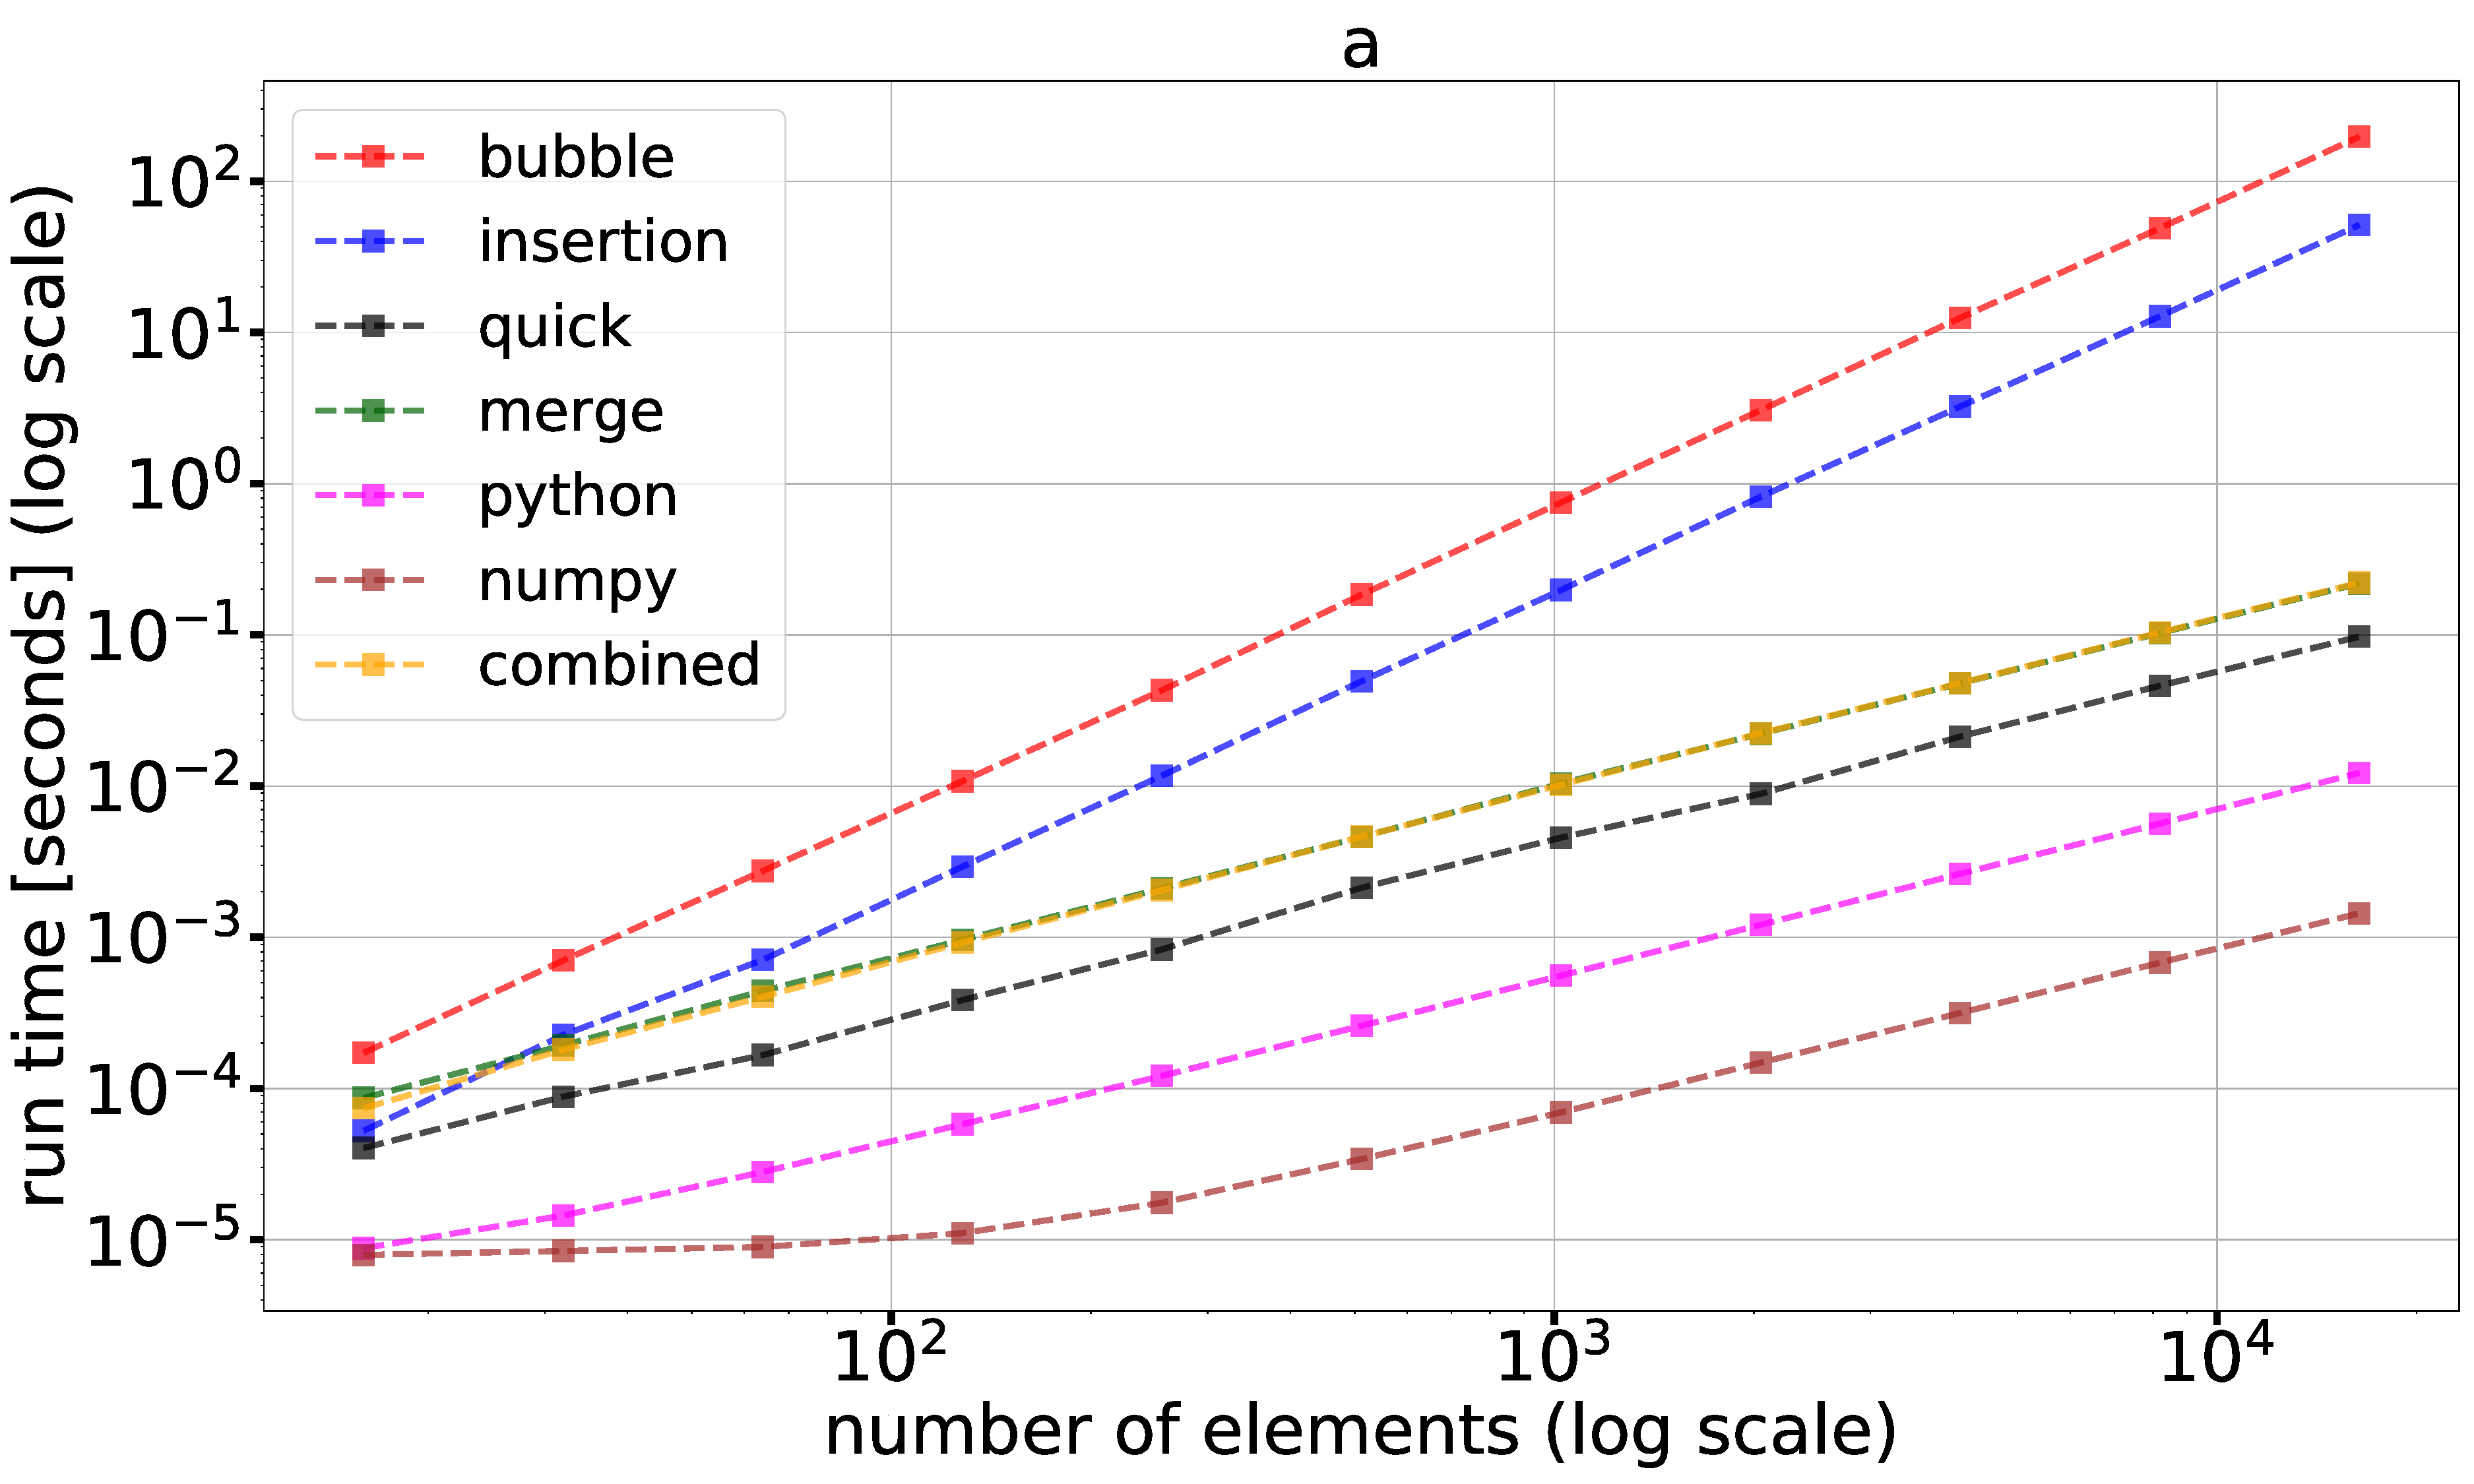
\includegraphics[width=84mm]{../figures/all_sorts_random_logscale.pdf}
  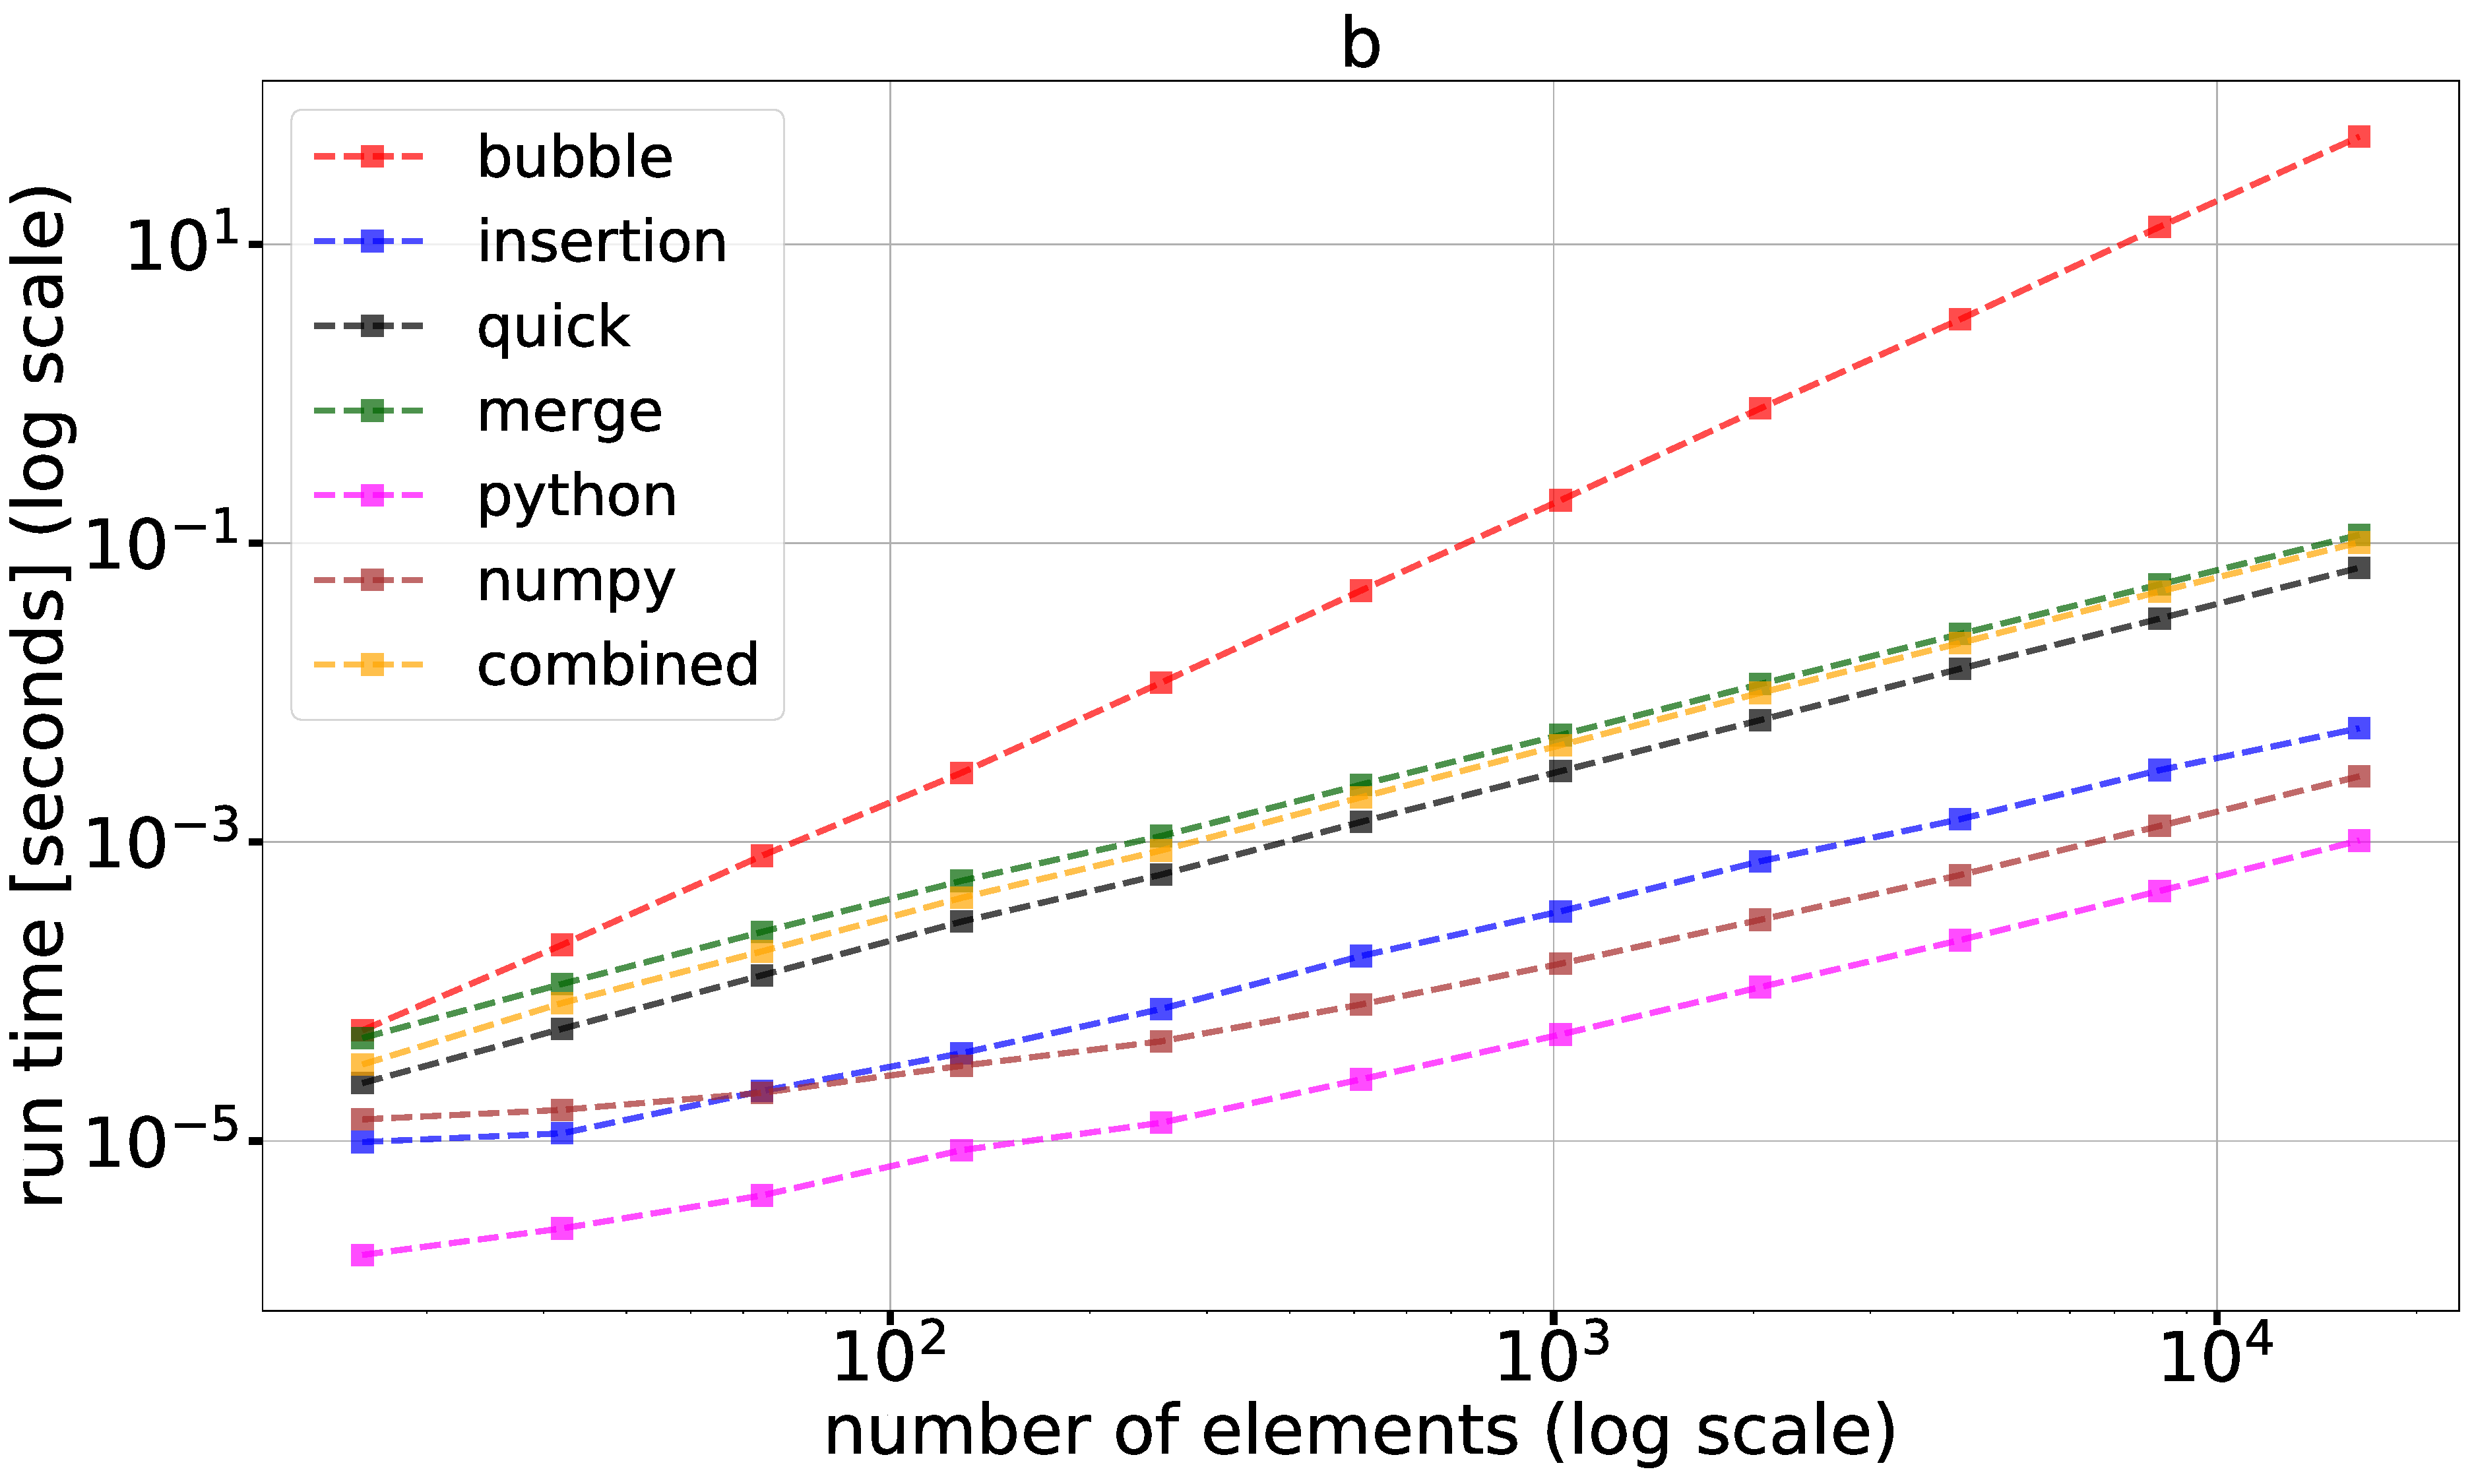
\includegraphics[width=84mm]{../figures/all_sorts_sorted_logscale.pdf}
  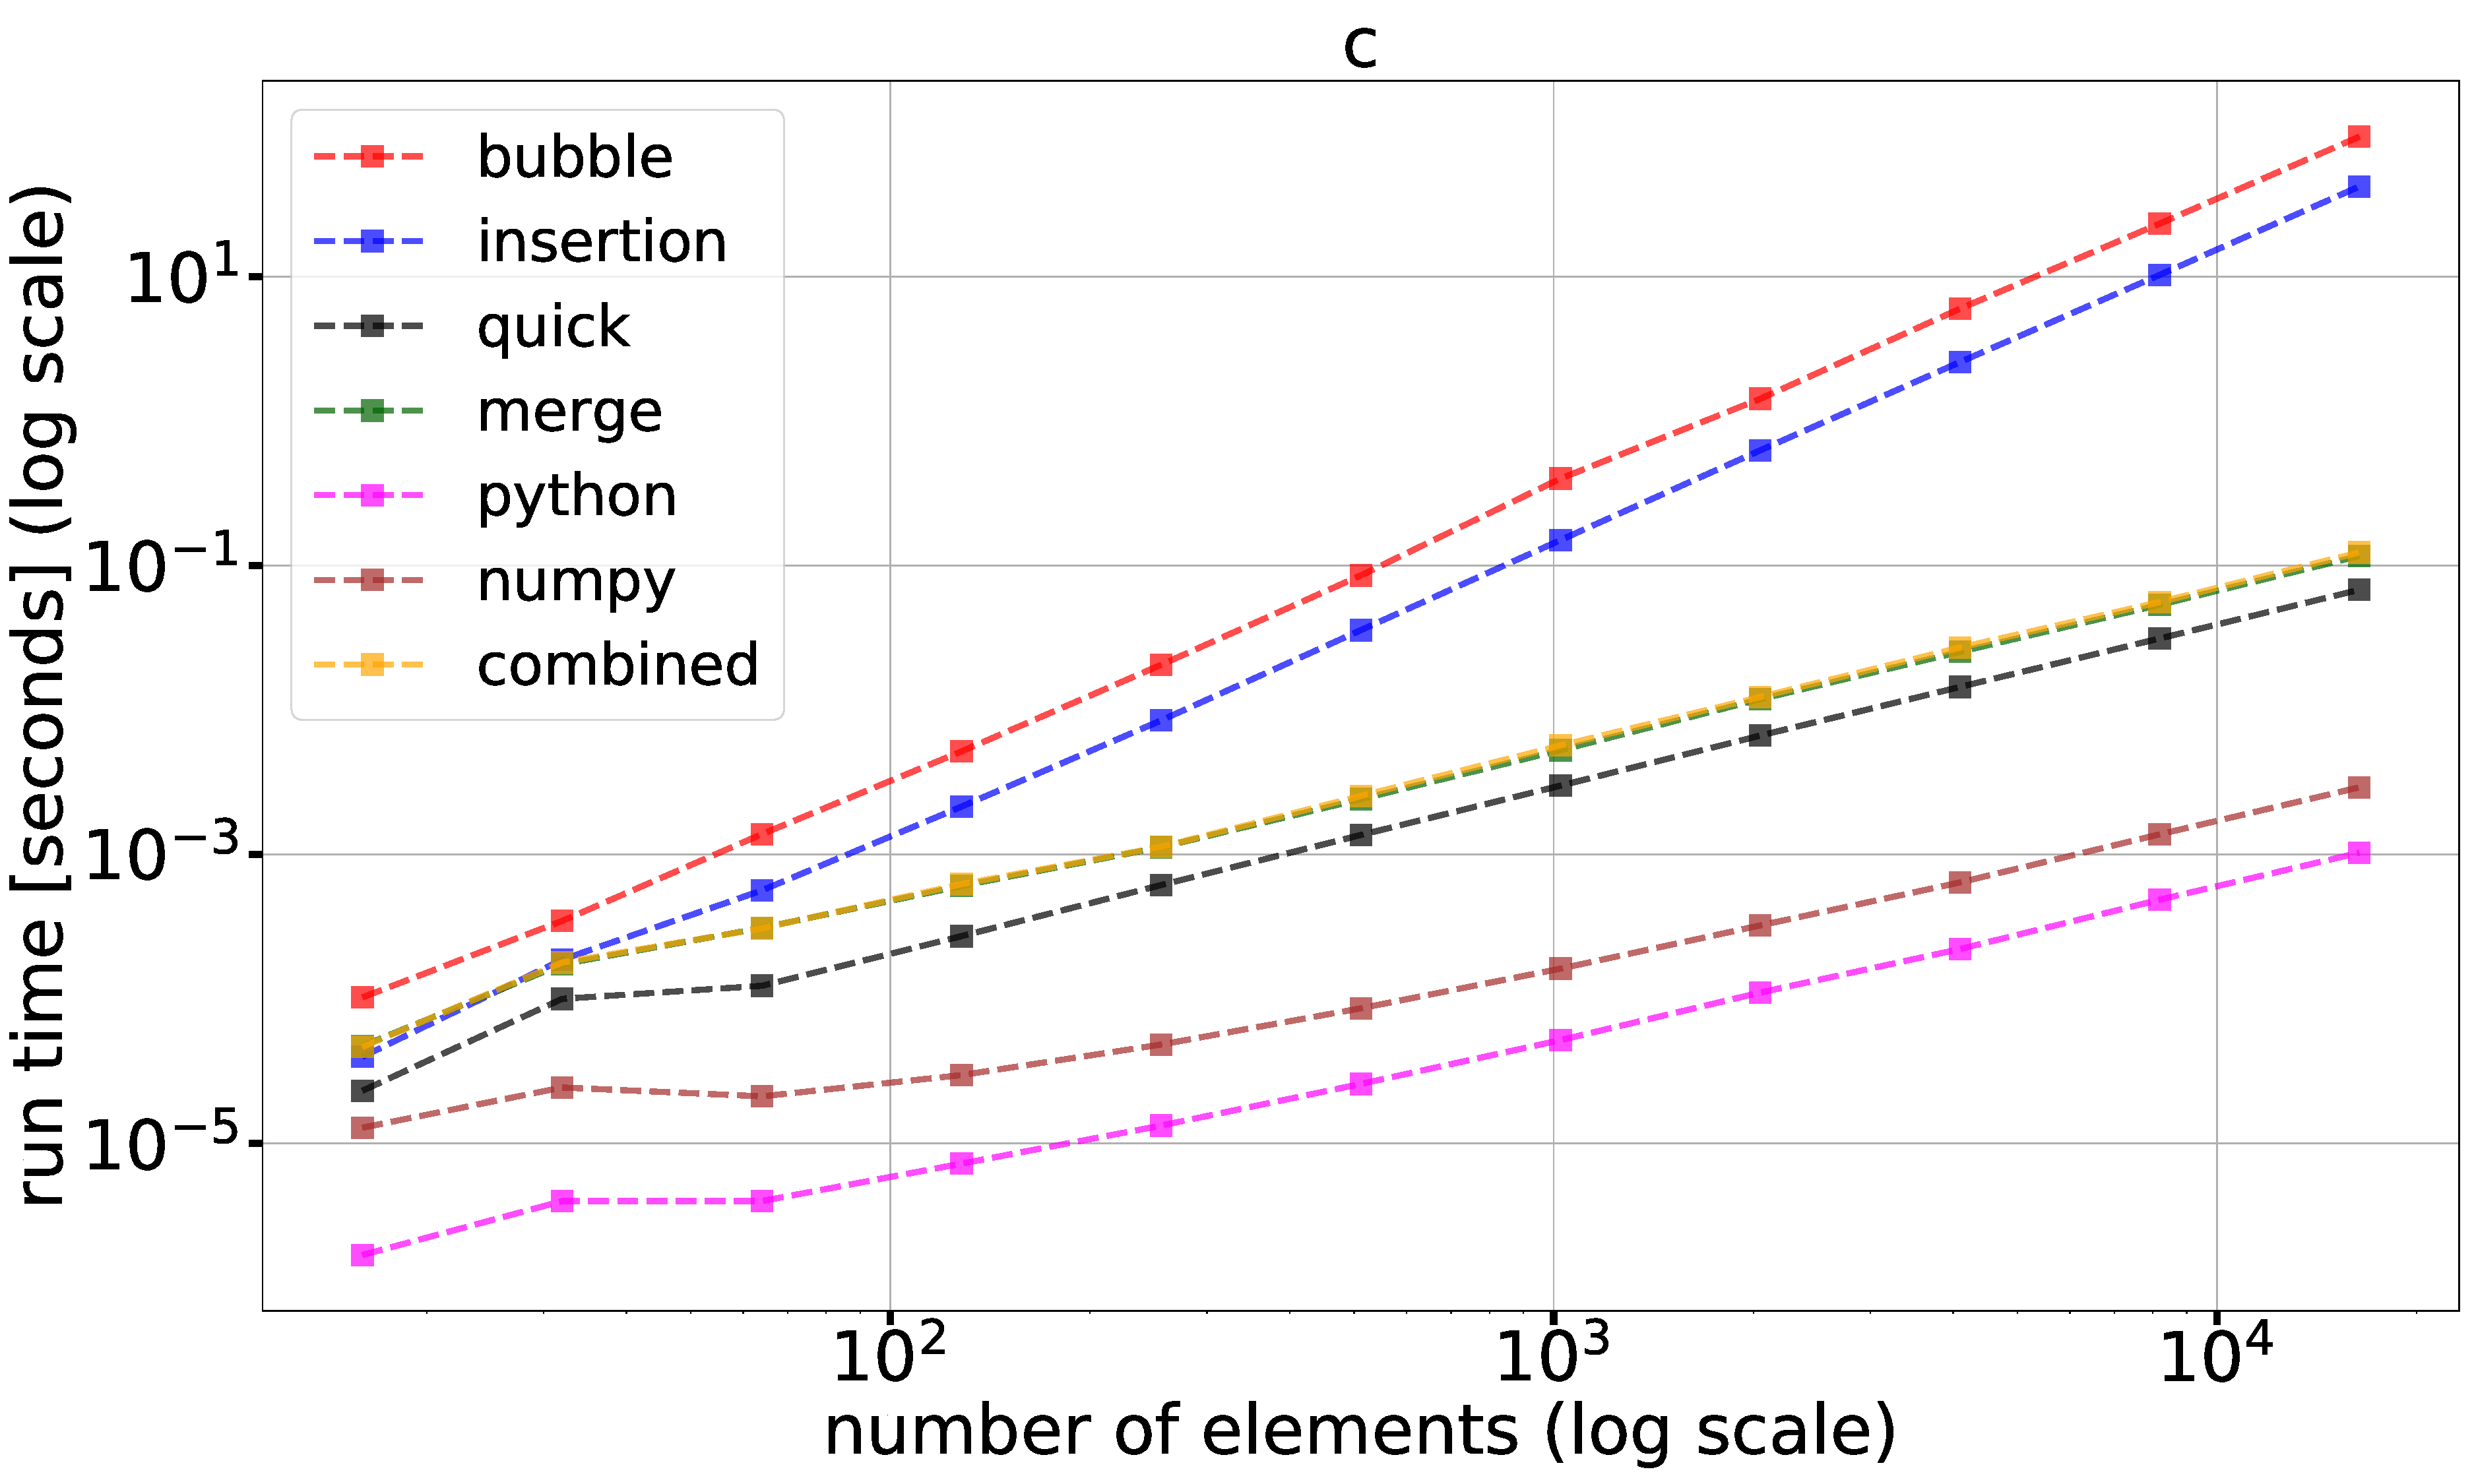
\includegraphics[width=84mm]{../figures/all_sorts_reverse_logscale.pdf}
  % figure captions below figure
  \caption{Comparison between all algorithms using a)random, b)sorted and c)reversed data. Dashed lines are depicted between the points for better illustration of trends.}
  \label{fig:fig_all}
\end{figure}

\begin{figure}
  \centering
  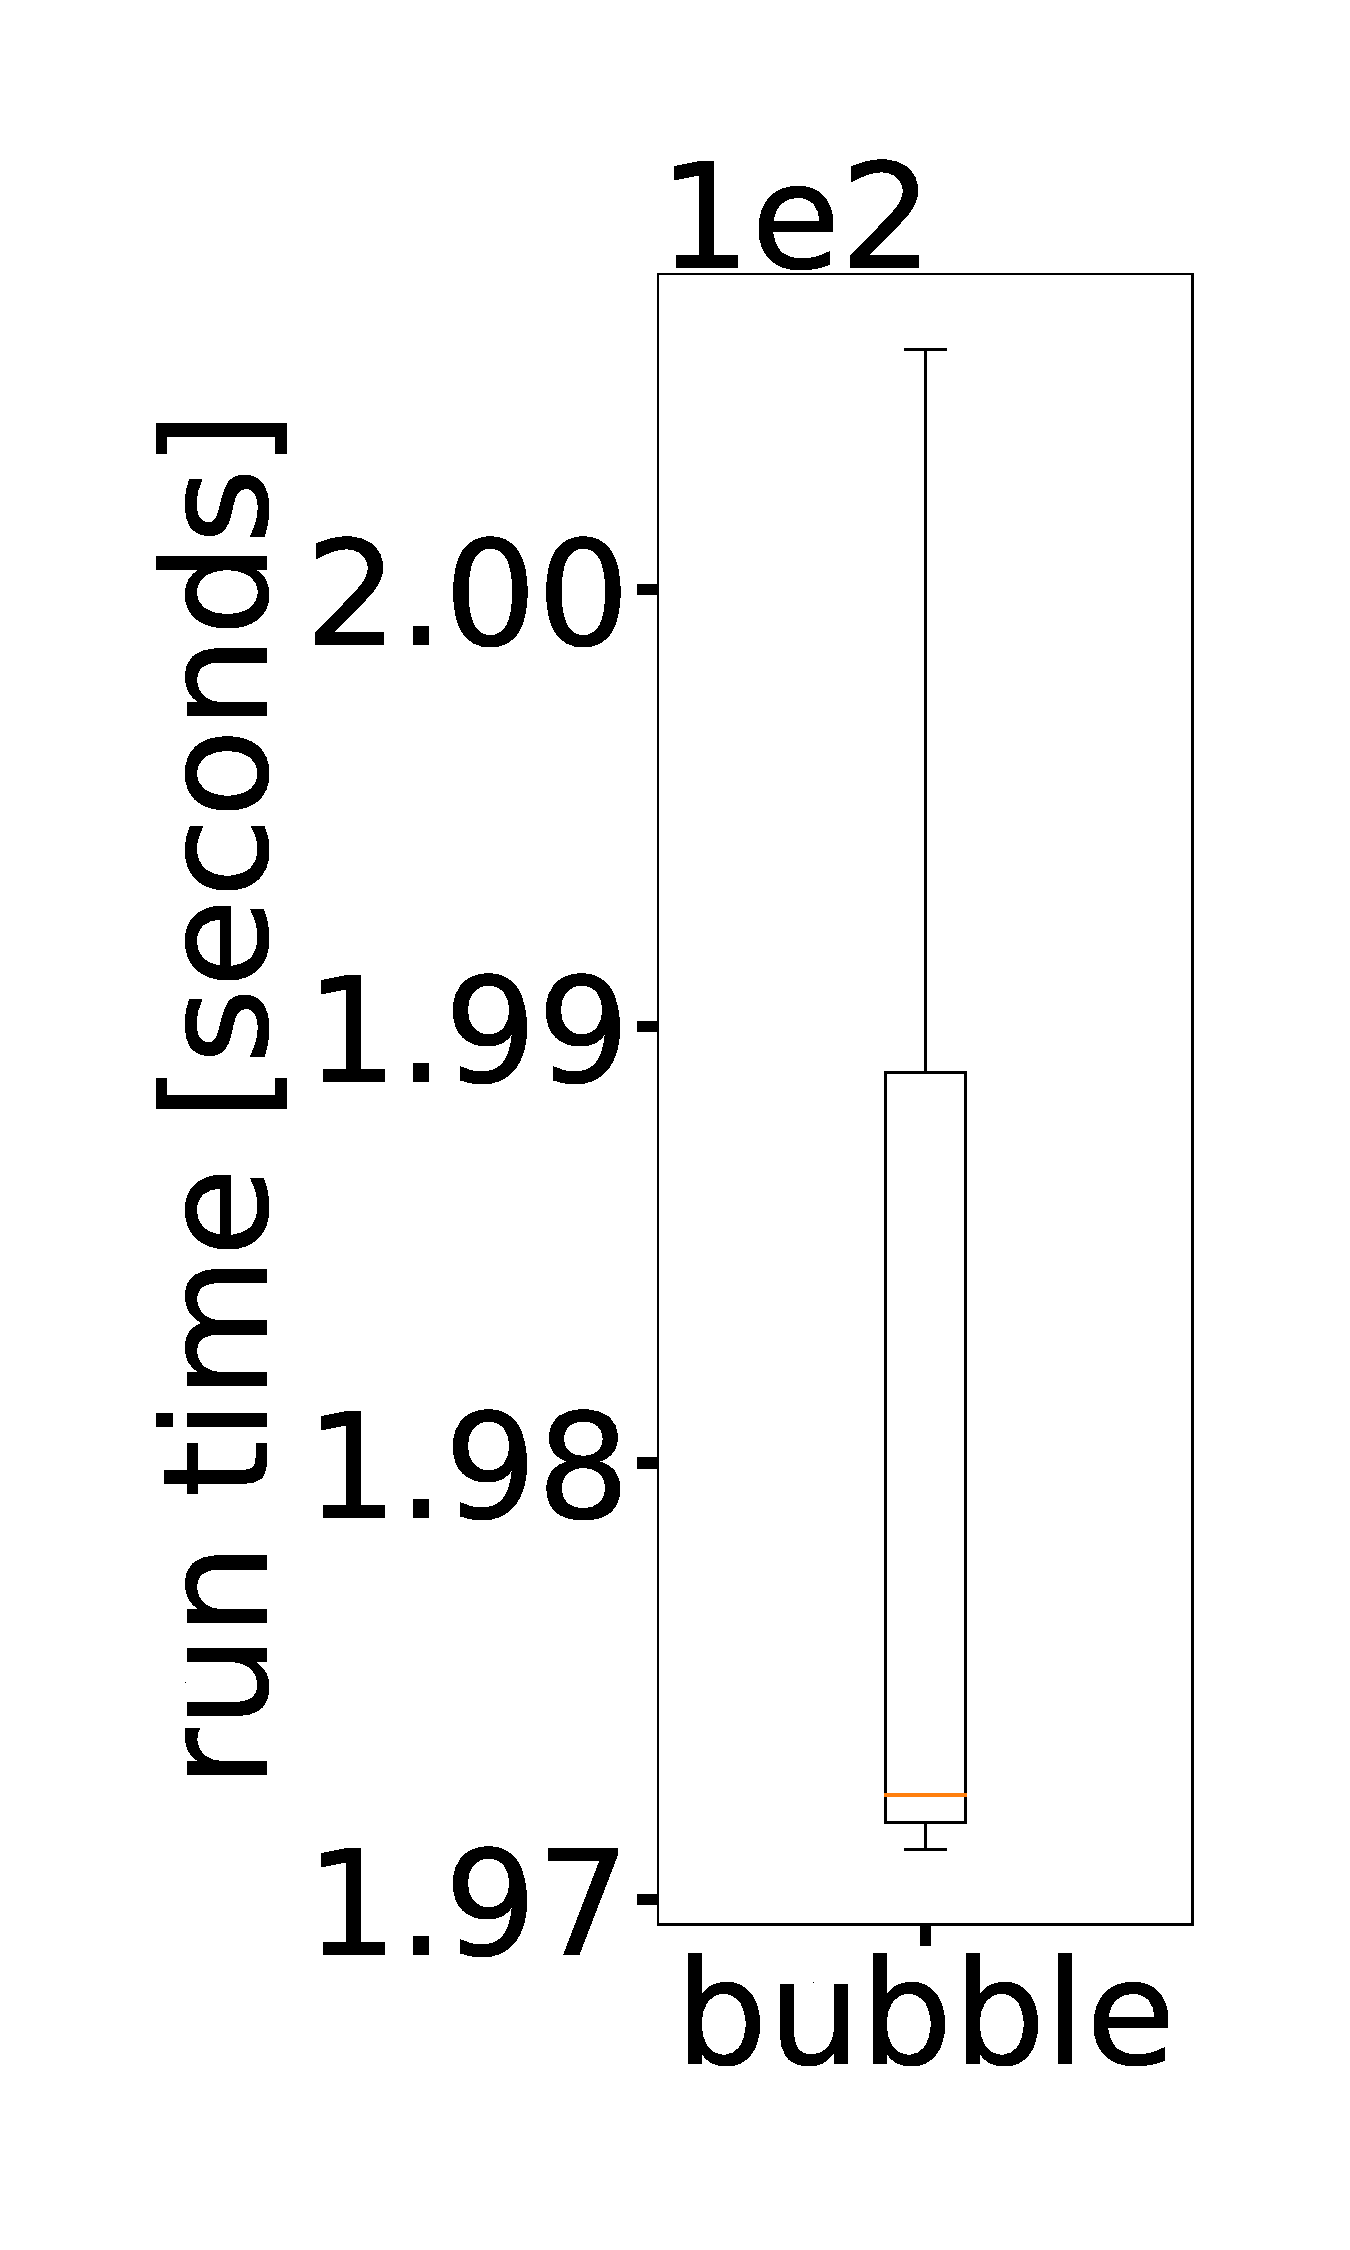
\includegraphics[width=15mm, height=30mm]{../figures/all_random_bubble_box.pdf}
  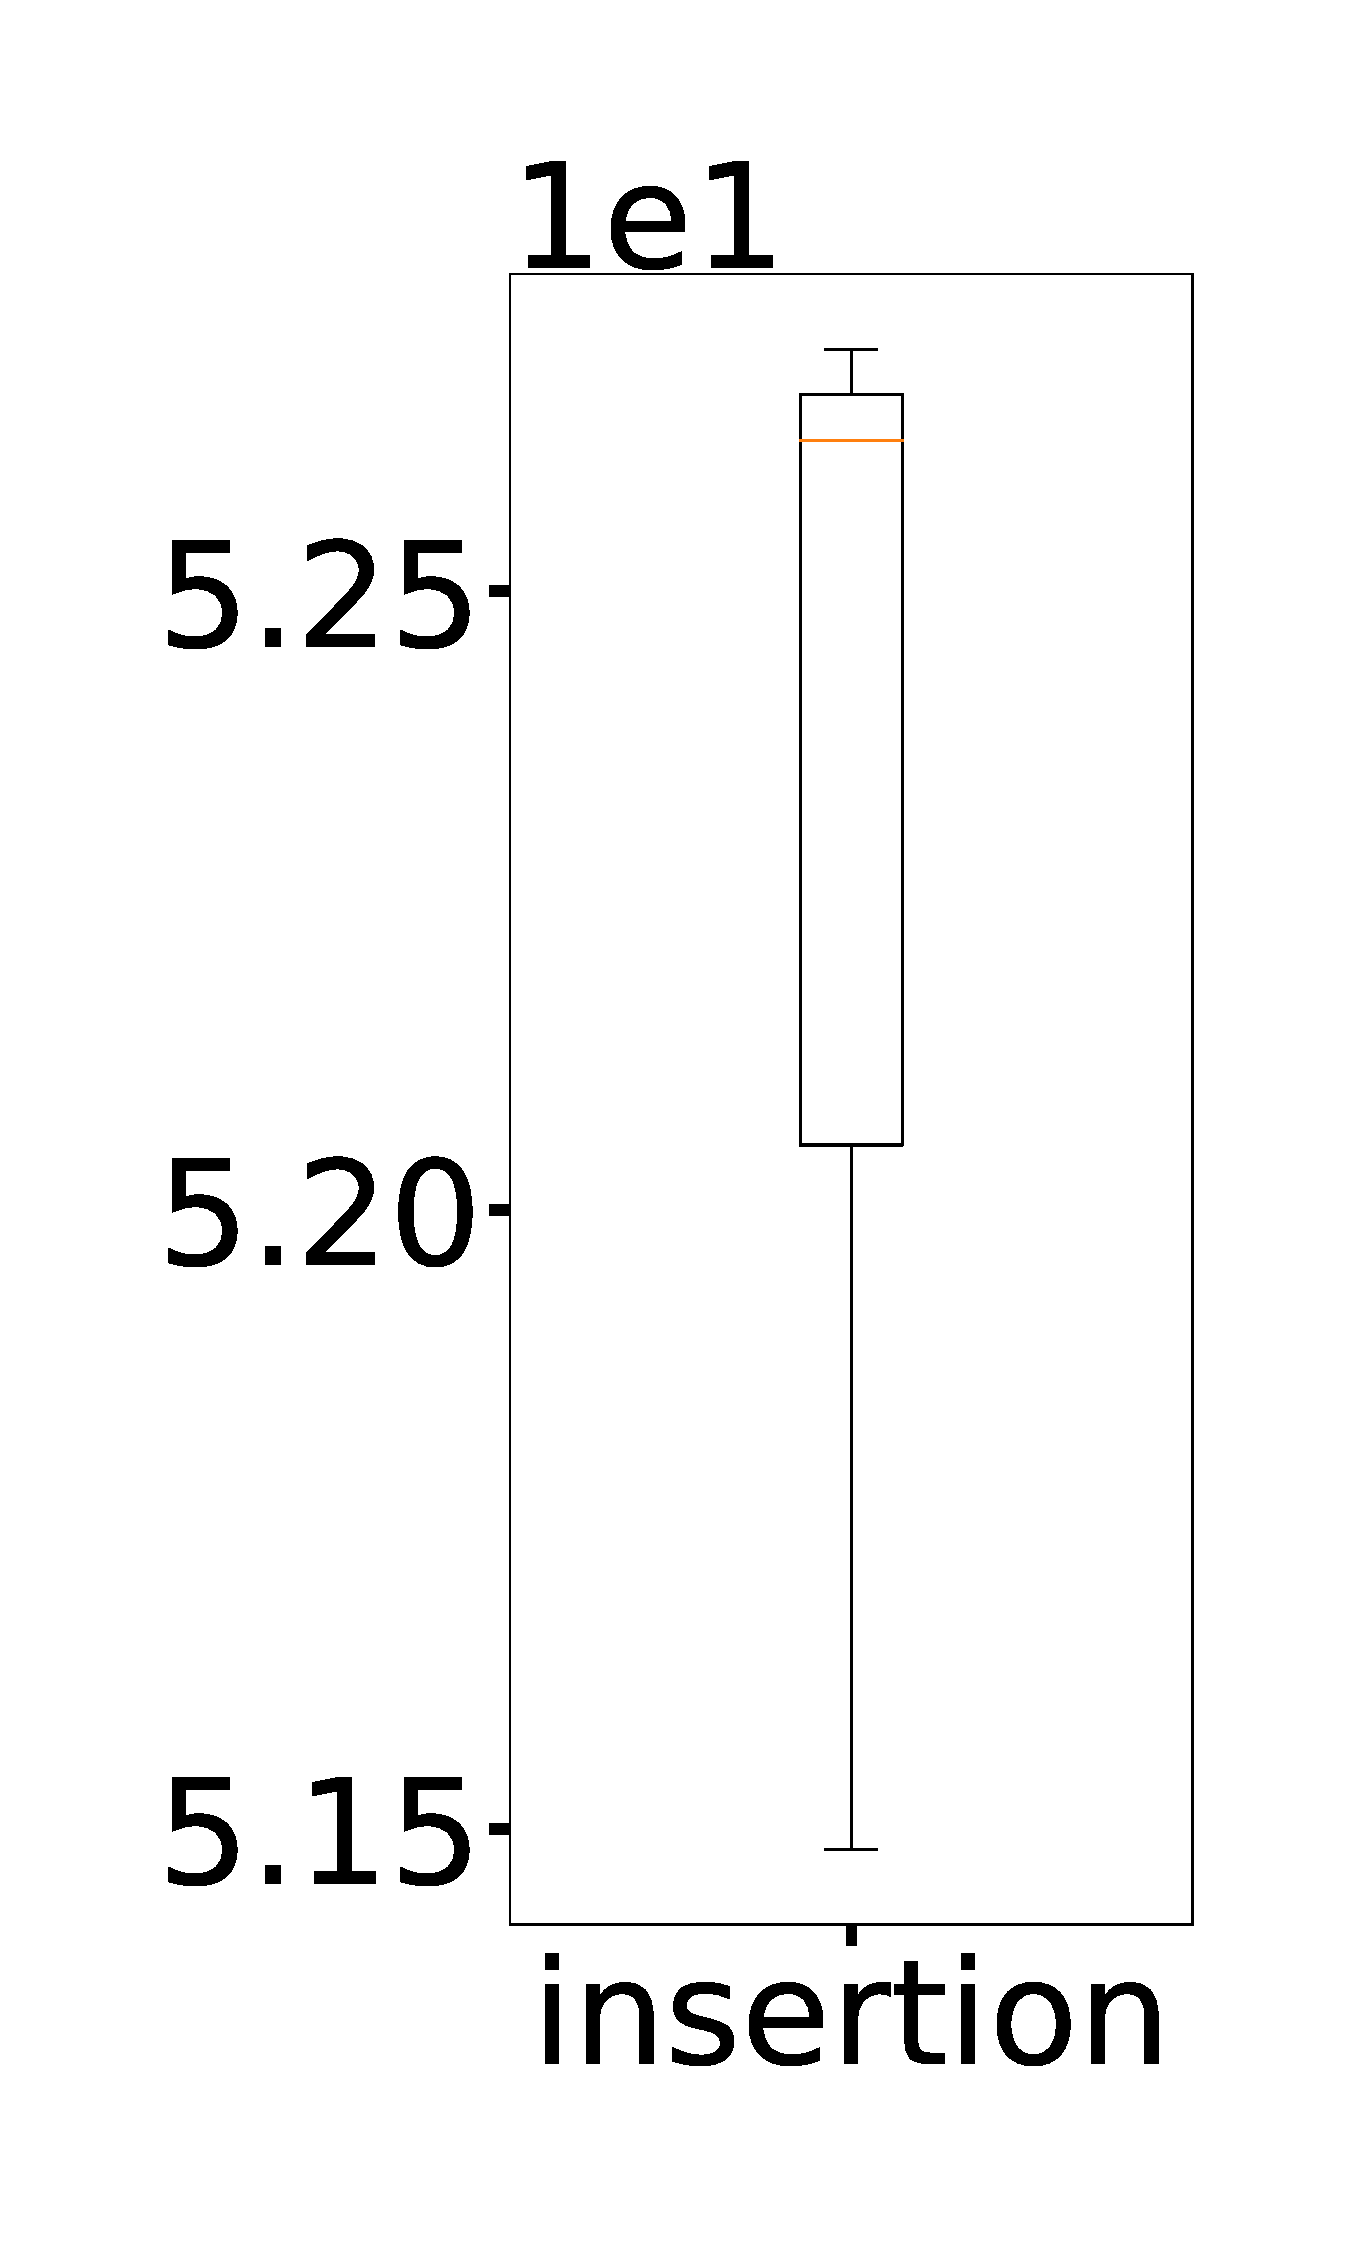
\includegraphics[width=15mm, height=30mm]{../figures/all_random_insertion_box.pdf}
  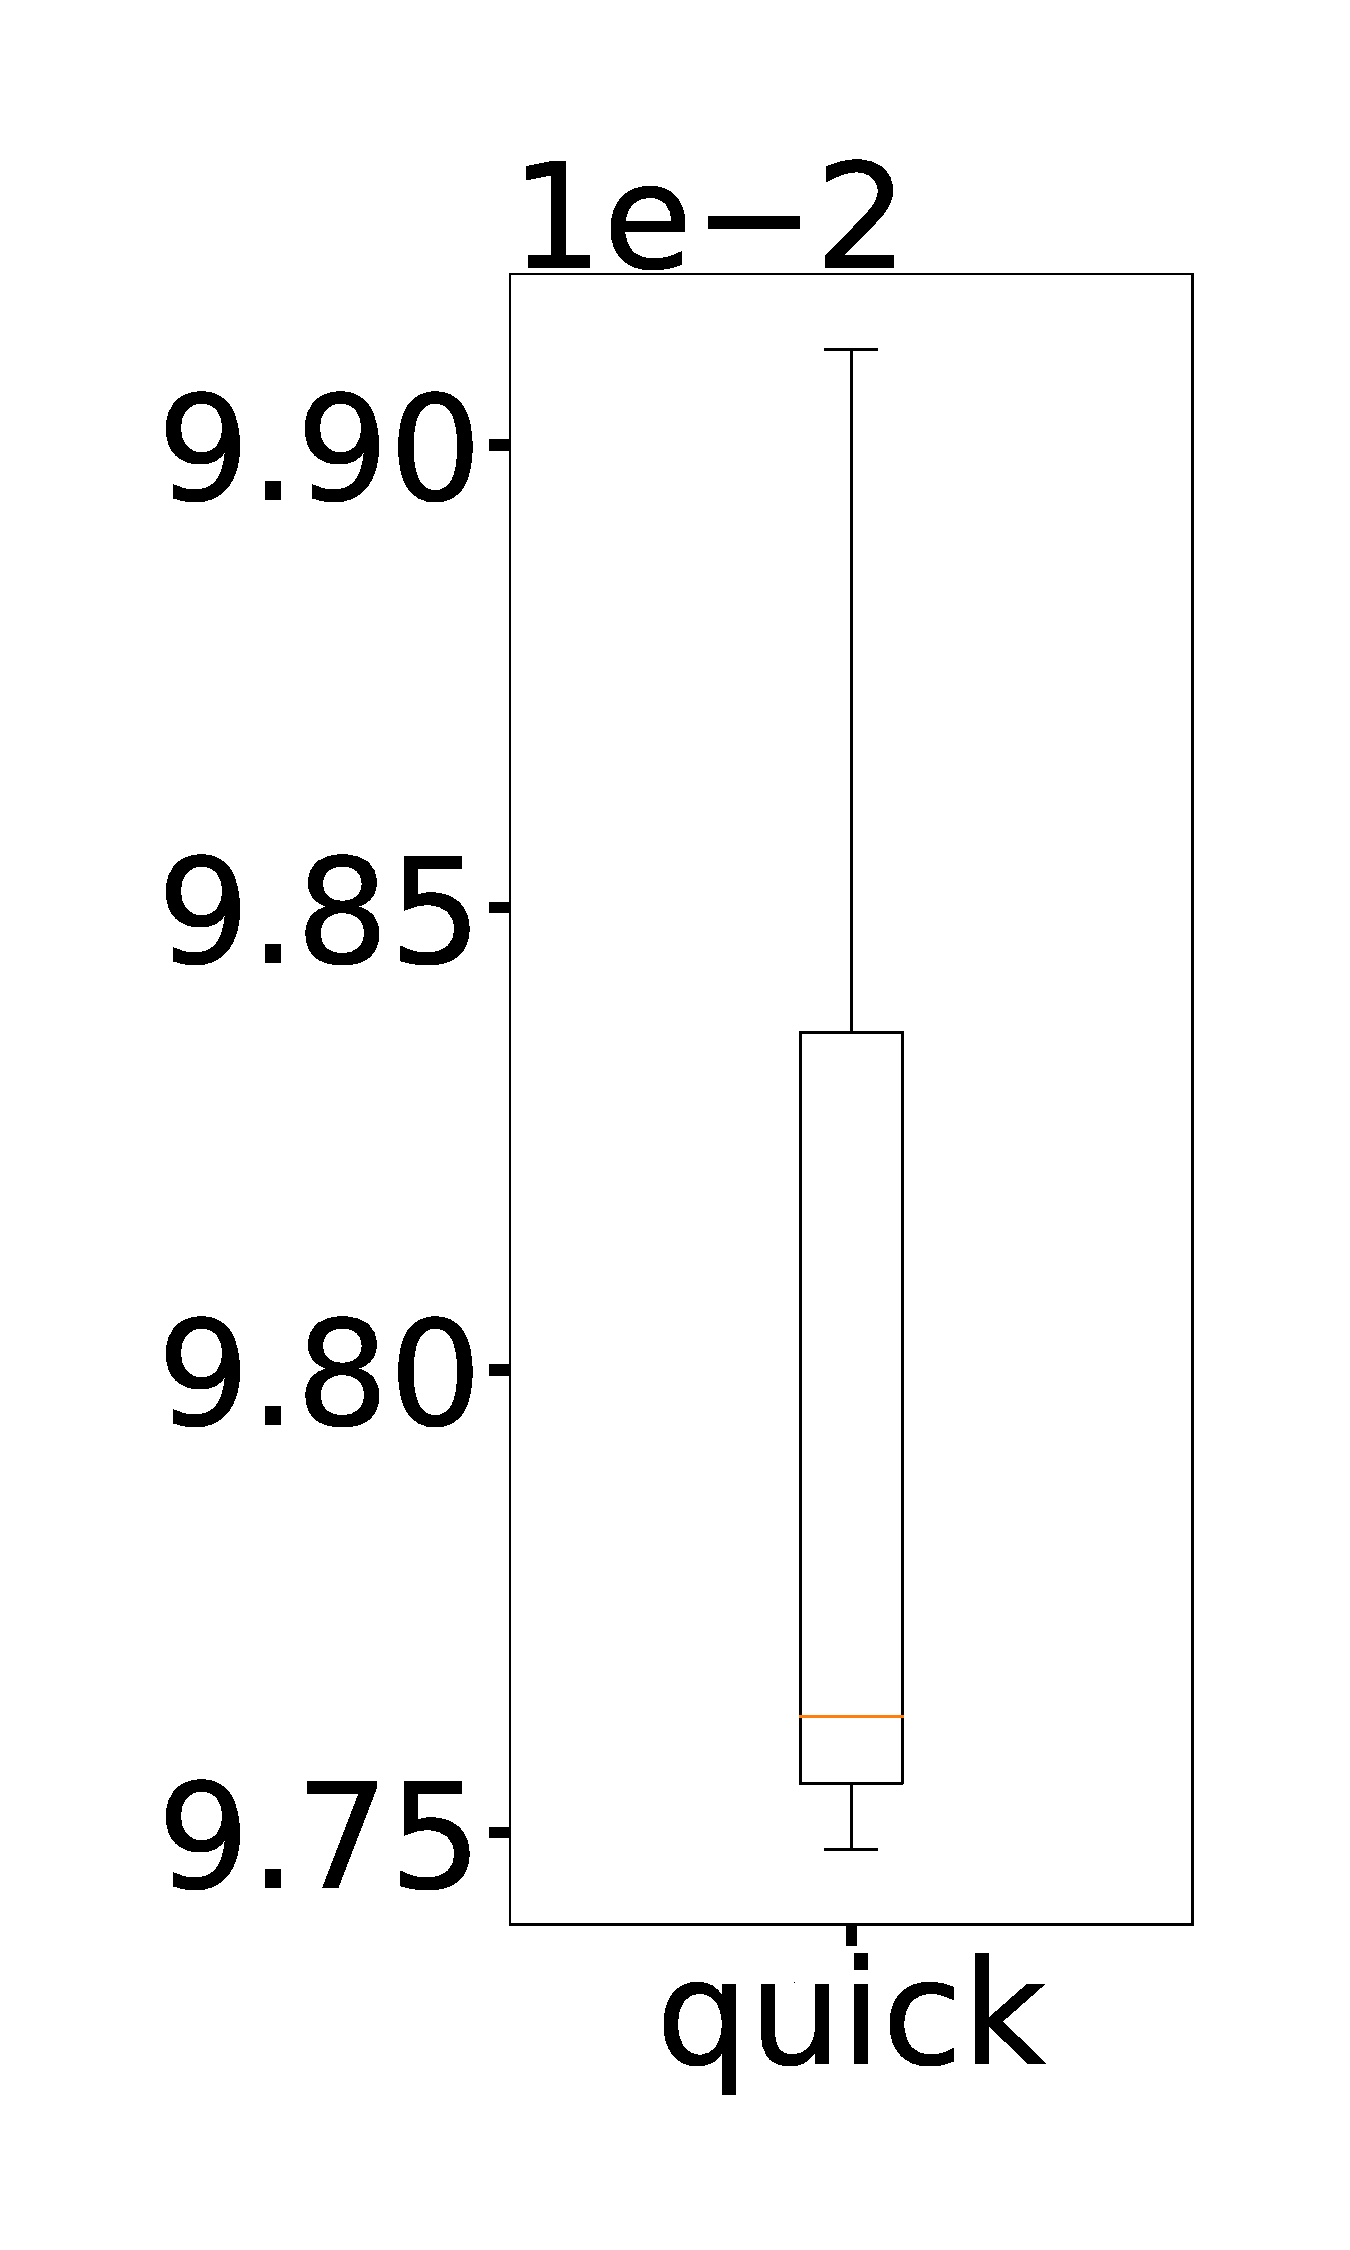
\includegraphics[width=15mm, height=30mm]{../figures/all_random_quick_box.pdf}
  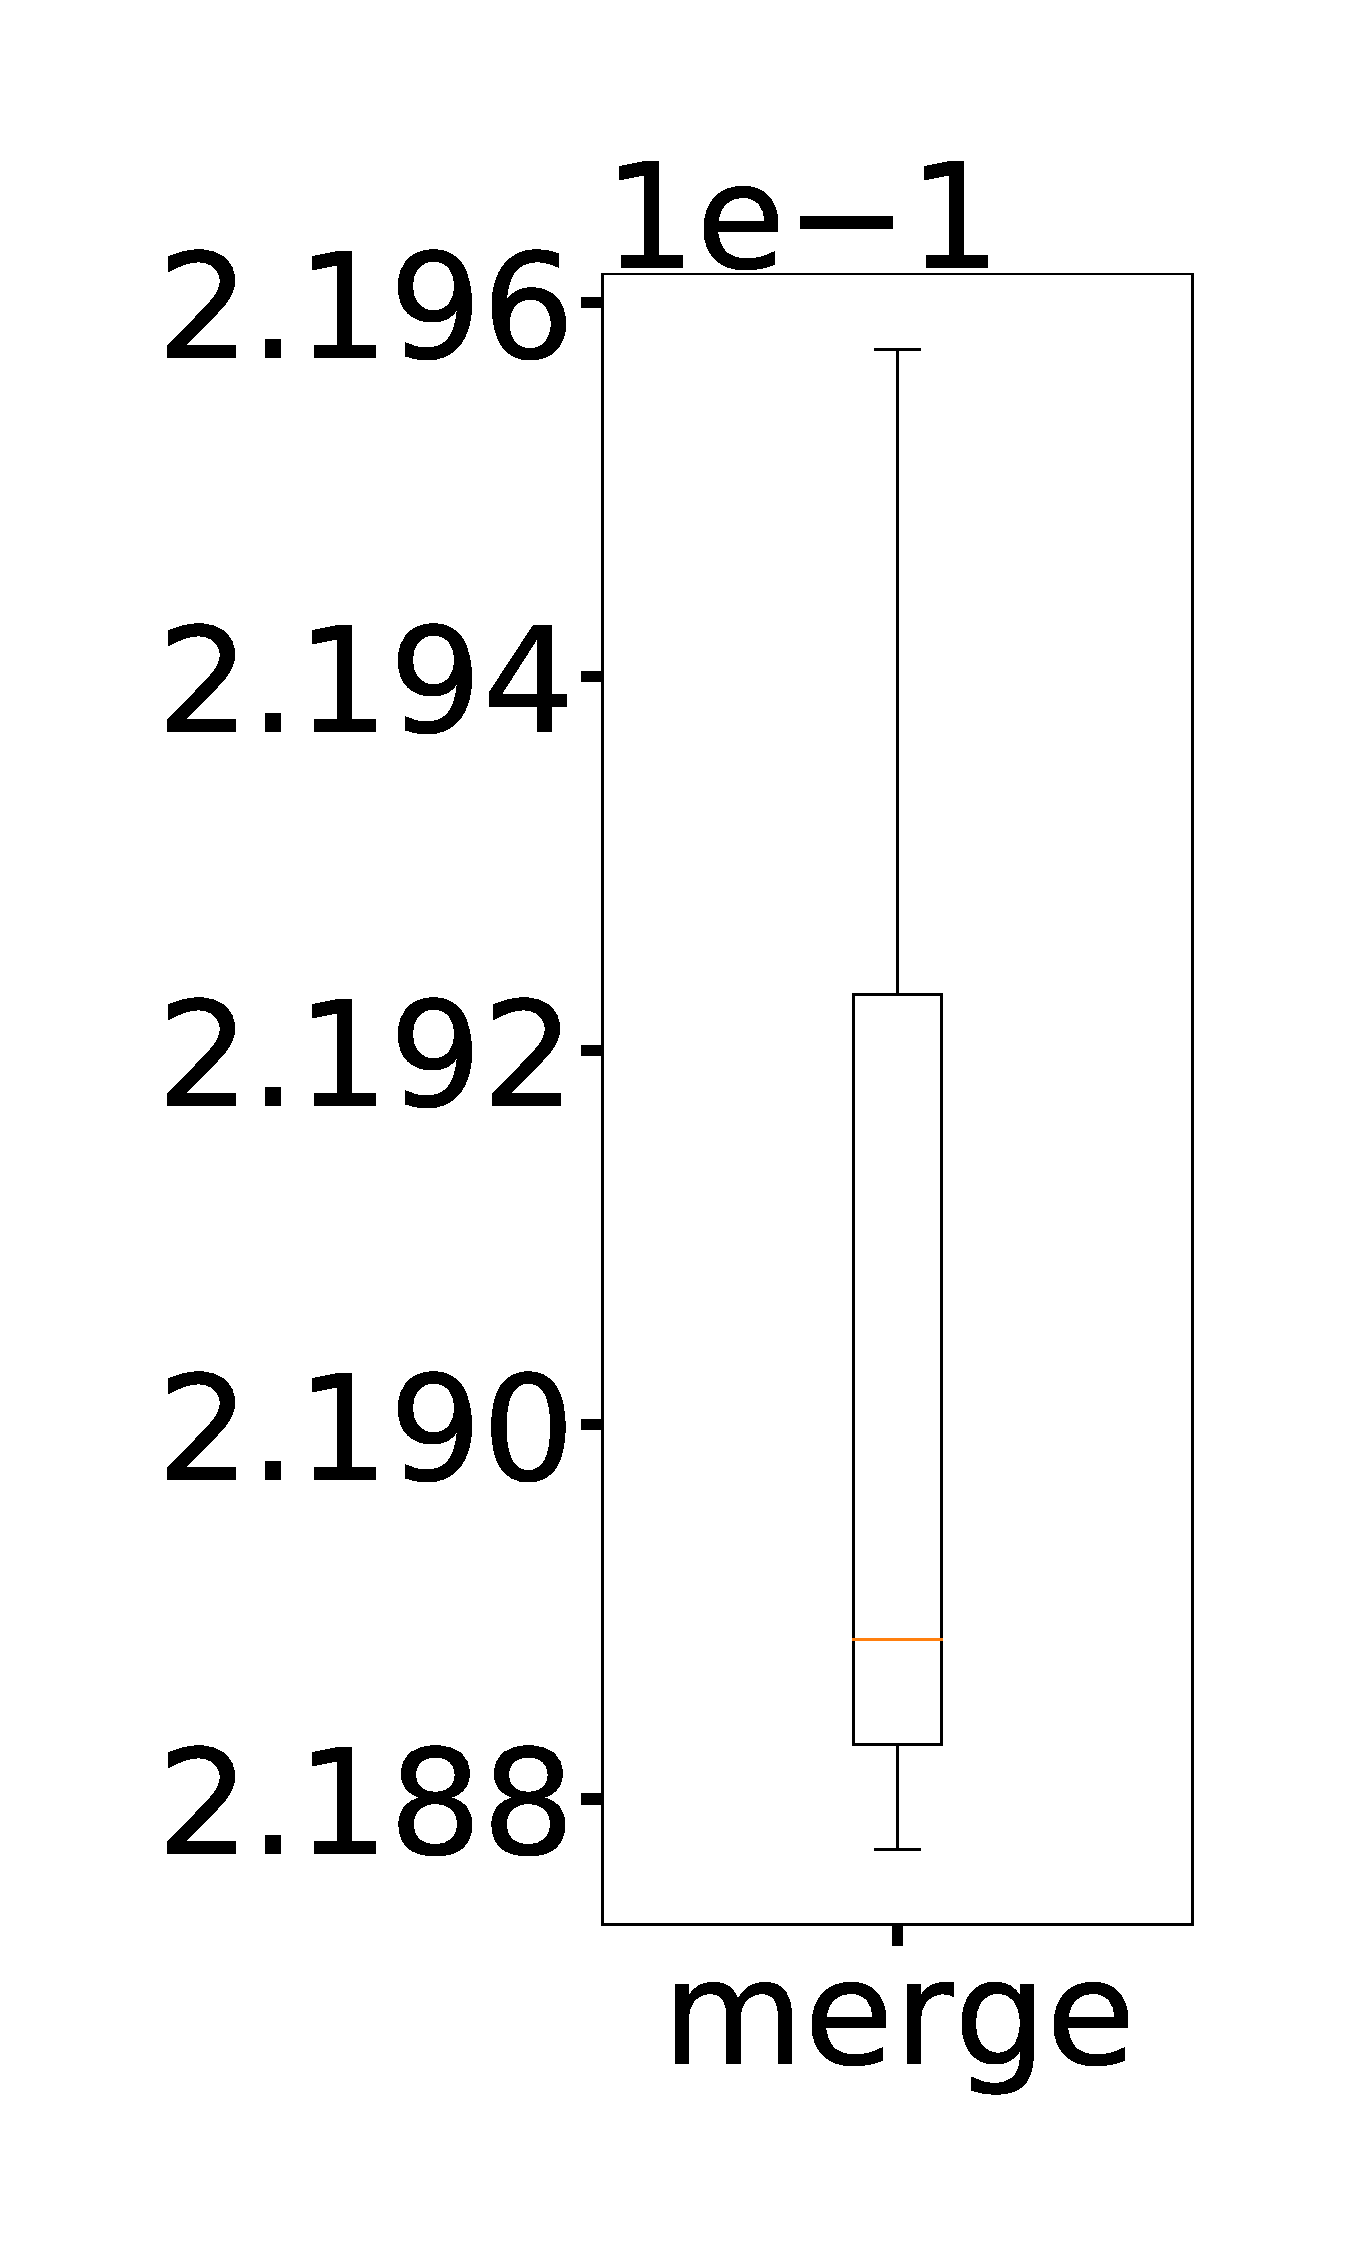
\includegraphics[width=15mm, height=30mm]{../figures/all_random_merge_box.pdf}
    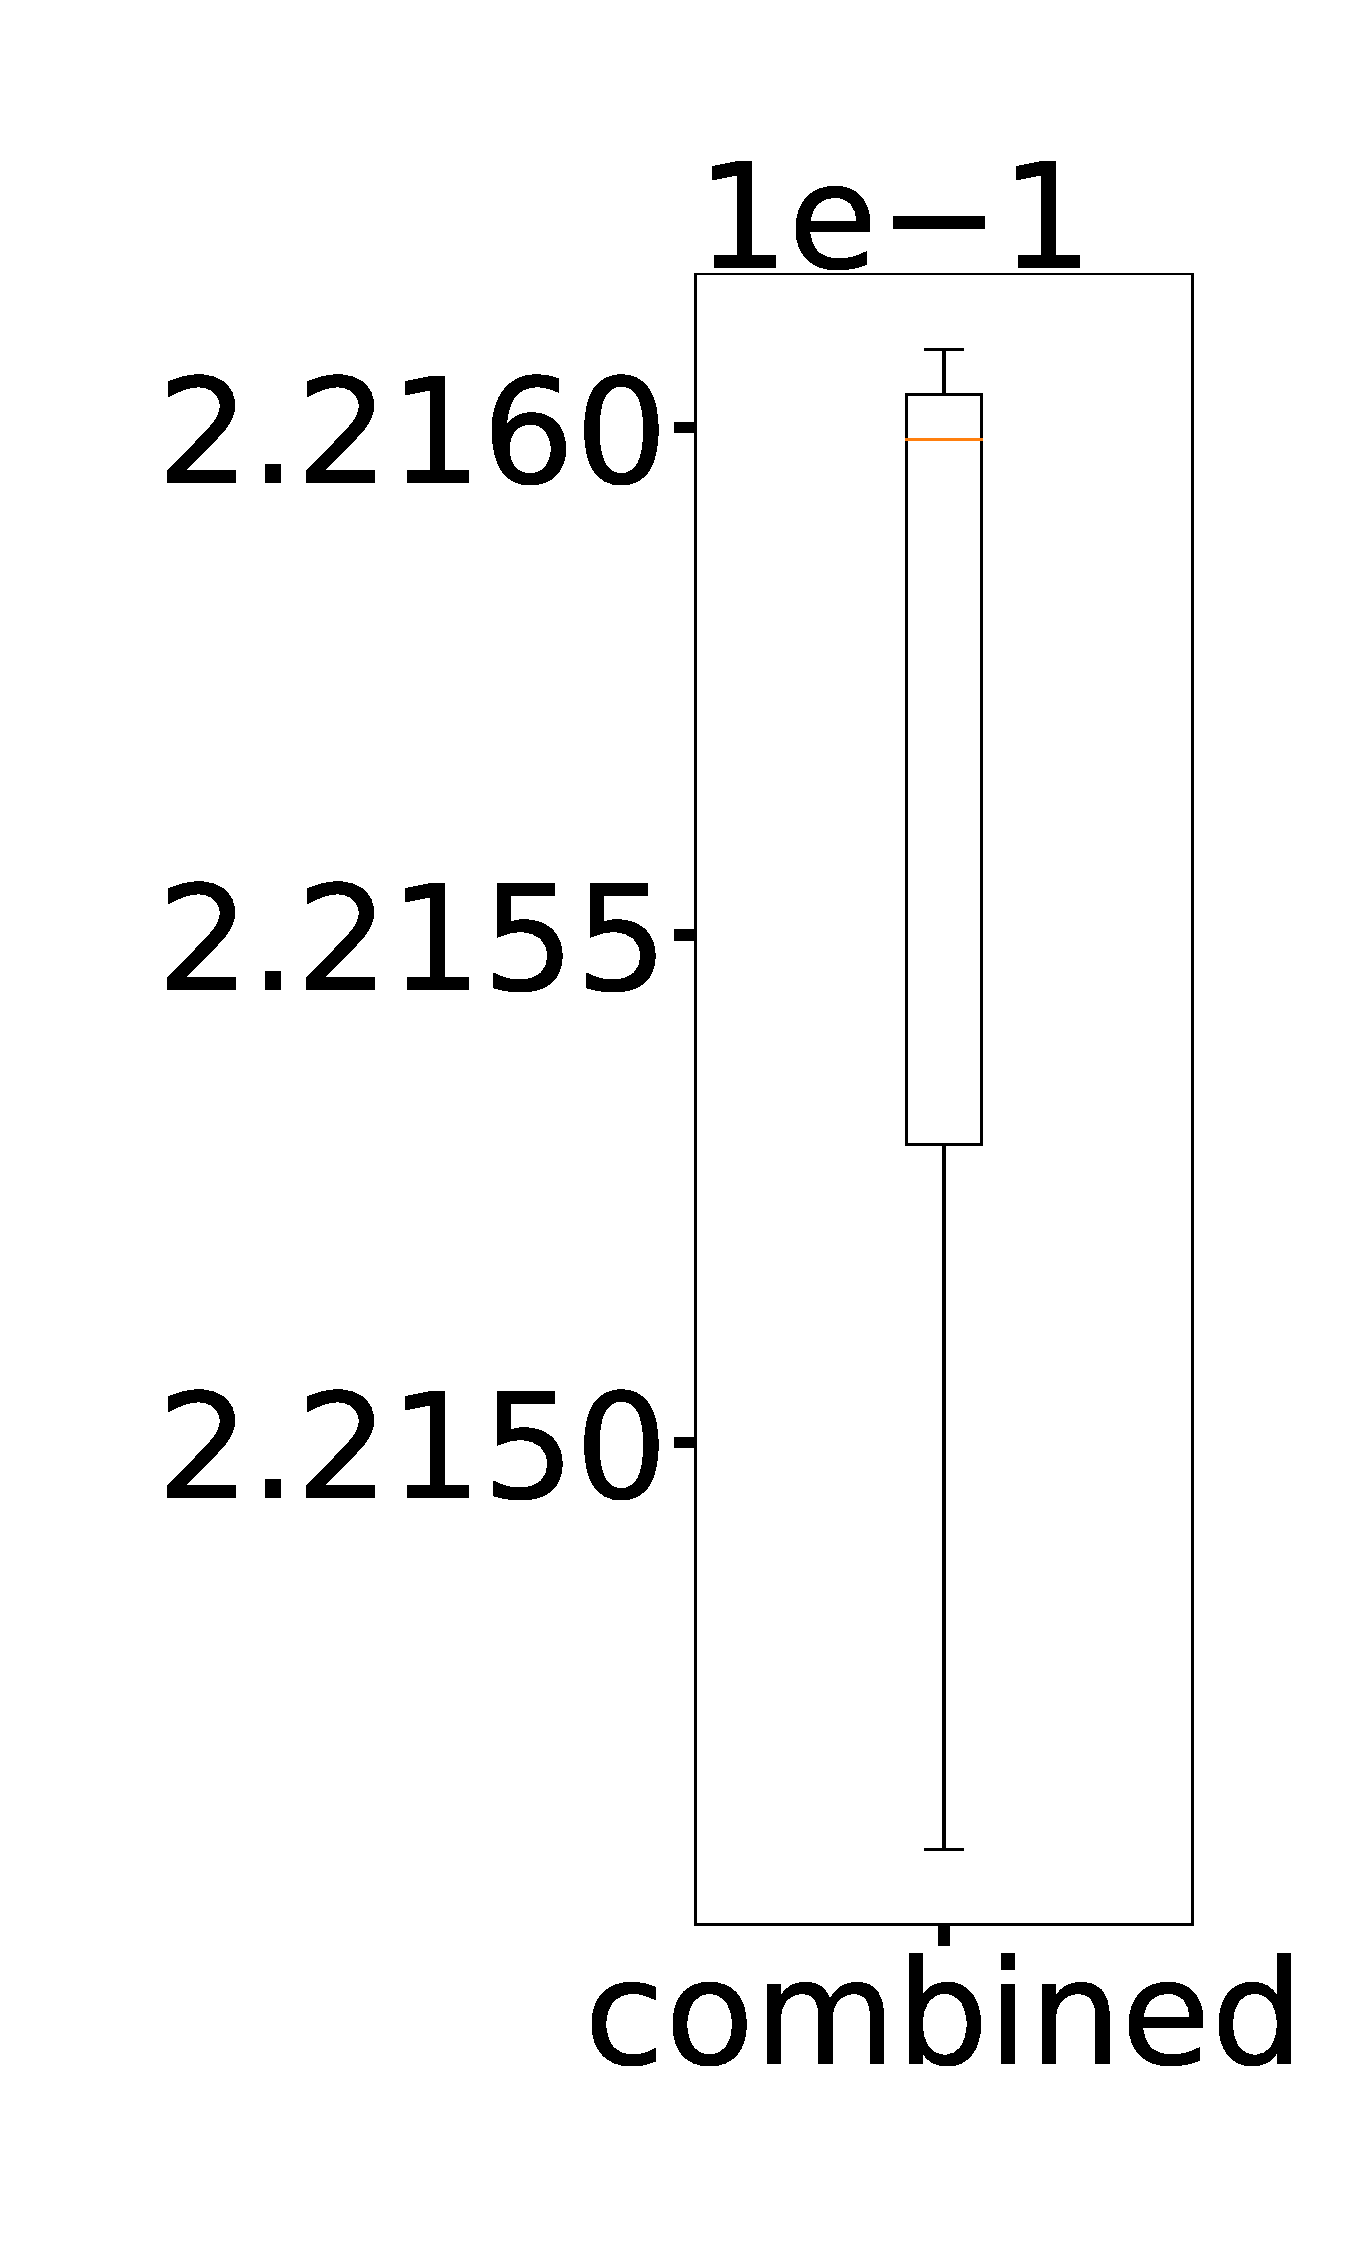
\includegraphics[width=15mm, height=30mm]{../figures/all_random_combined_box.pdf}

  % figure captions below figure
  \caption{Box-plots for Bubble-Sort, Insertion-Sort,  Quick-Sort, Merge-Sort and Merge-Insertion-Sort (combined sort).}
  \label{fig:fig_box}
\end{figure}

\subsection{Quadratic Sorts}
Figure~\ref{fig:quad} shows a comparison between Bubble-Sort and Insertion-Sort. Both sorting algorithms follow quadratic run-time except in best case of Insertion-Sort. Insertion-Sort follows linear run-time in sorting already sorted data. Overall, Insertion-Sort is $4$ times faster than Bubble-Sort in sorting random data. Insertion-Sort also is $2$ times faster than Bubble-Sort in sorting reversed data. It is also noticed that Insertion-Sort and Bubble-Sort take longer run-time to sort random data than reversed data. Bubble-Sort is $2$ times faster in sorting random data than sorting reversed data. 

\begin{figure}
  \centering
  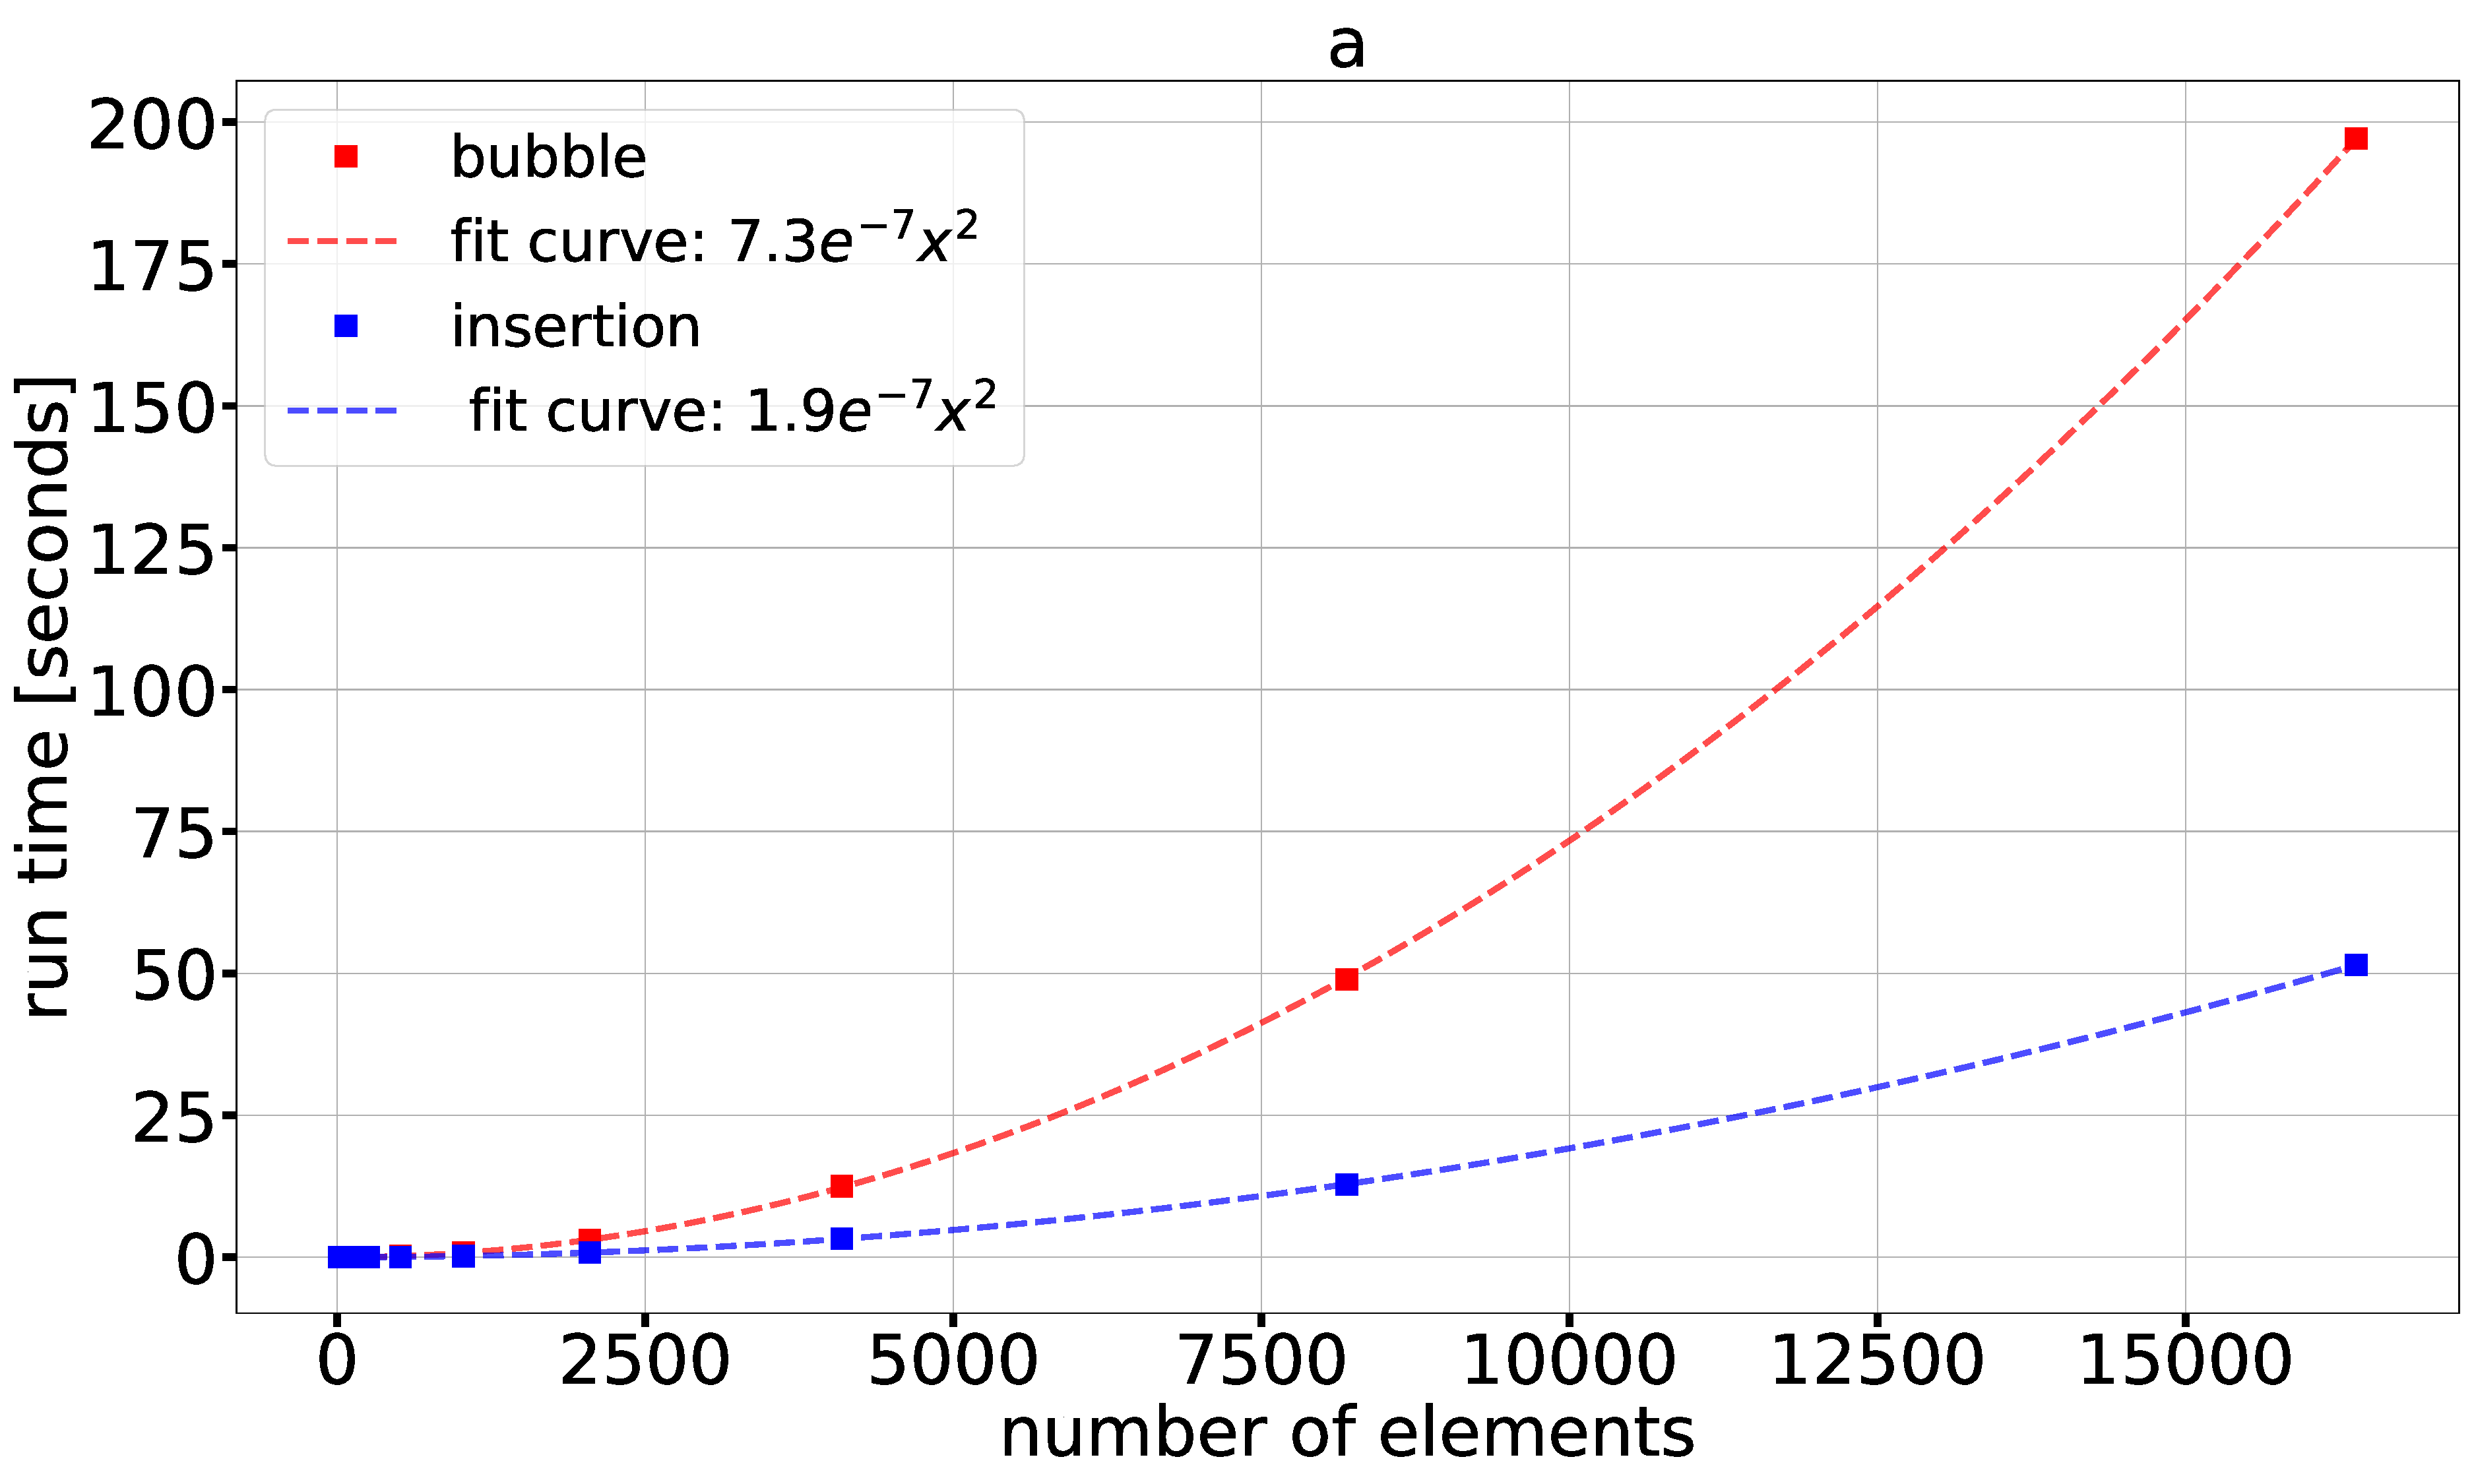
\includegraphics[width=84mm]{../figures/bubble_vs_insertion_random.pdf}
  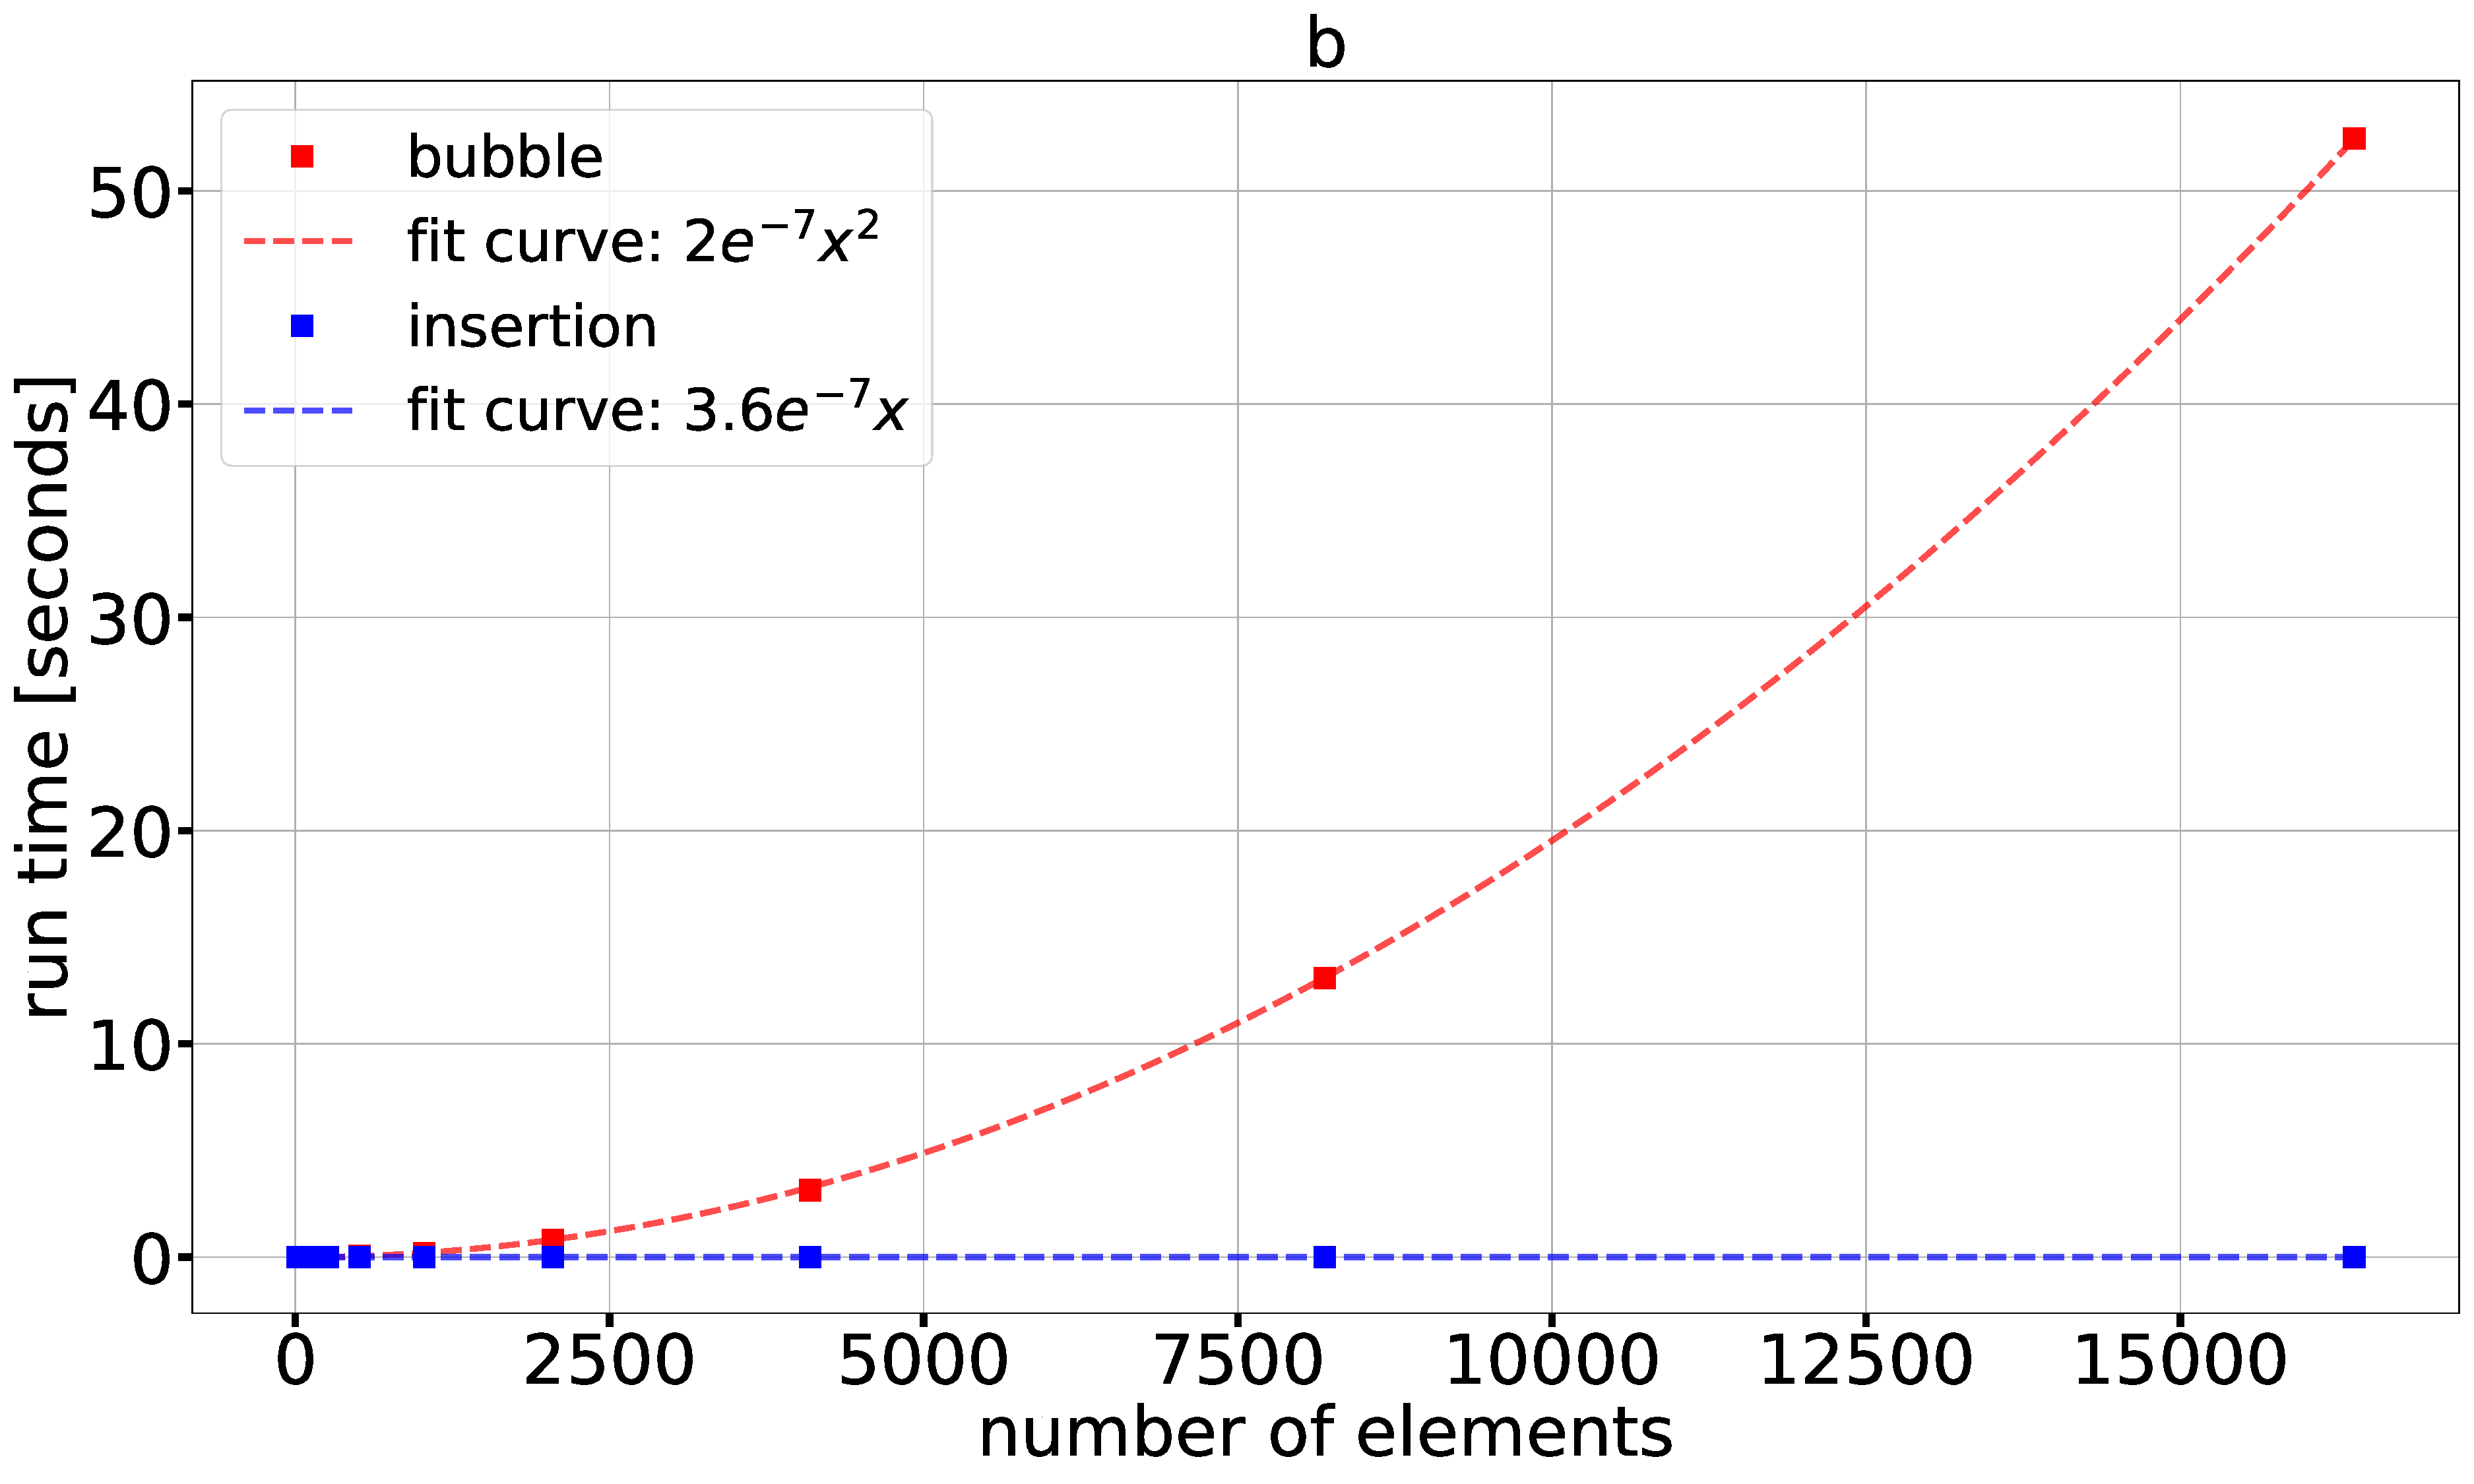
\includegraphics[width=84mm]{../figures/bubble_vs_insertion_sorted.pdf}
  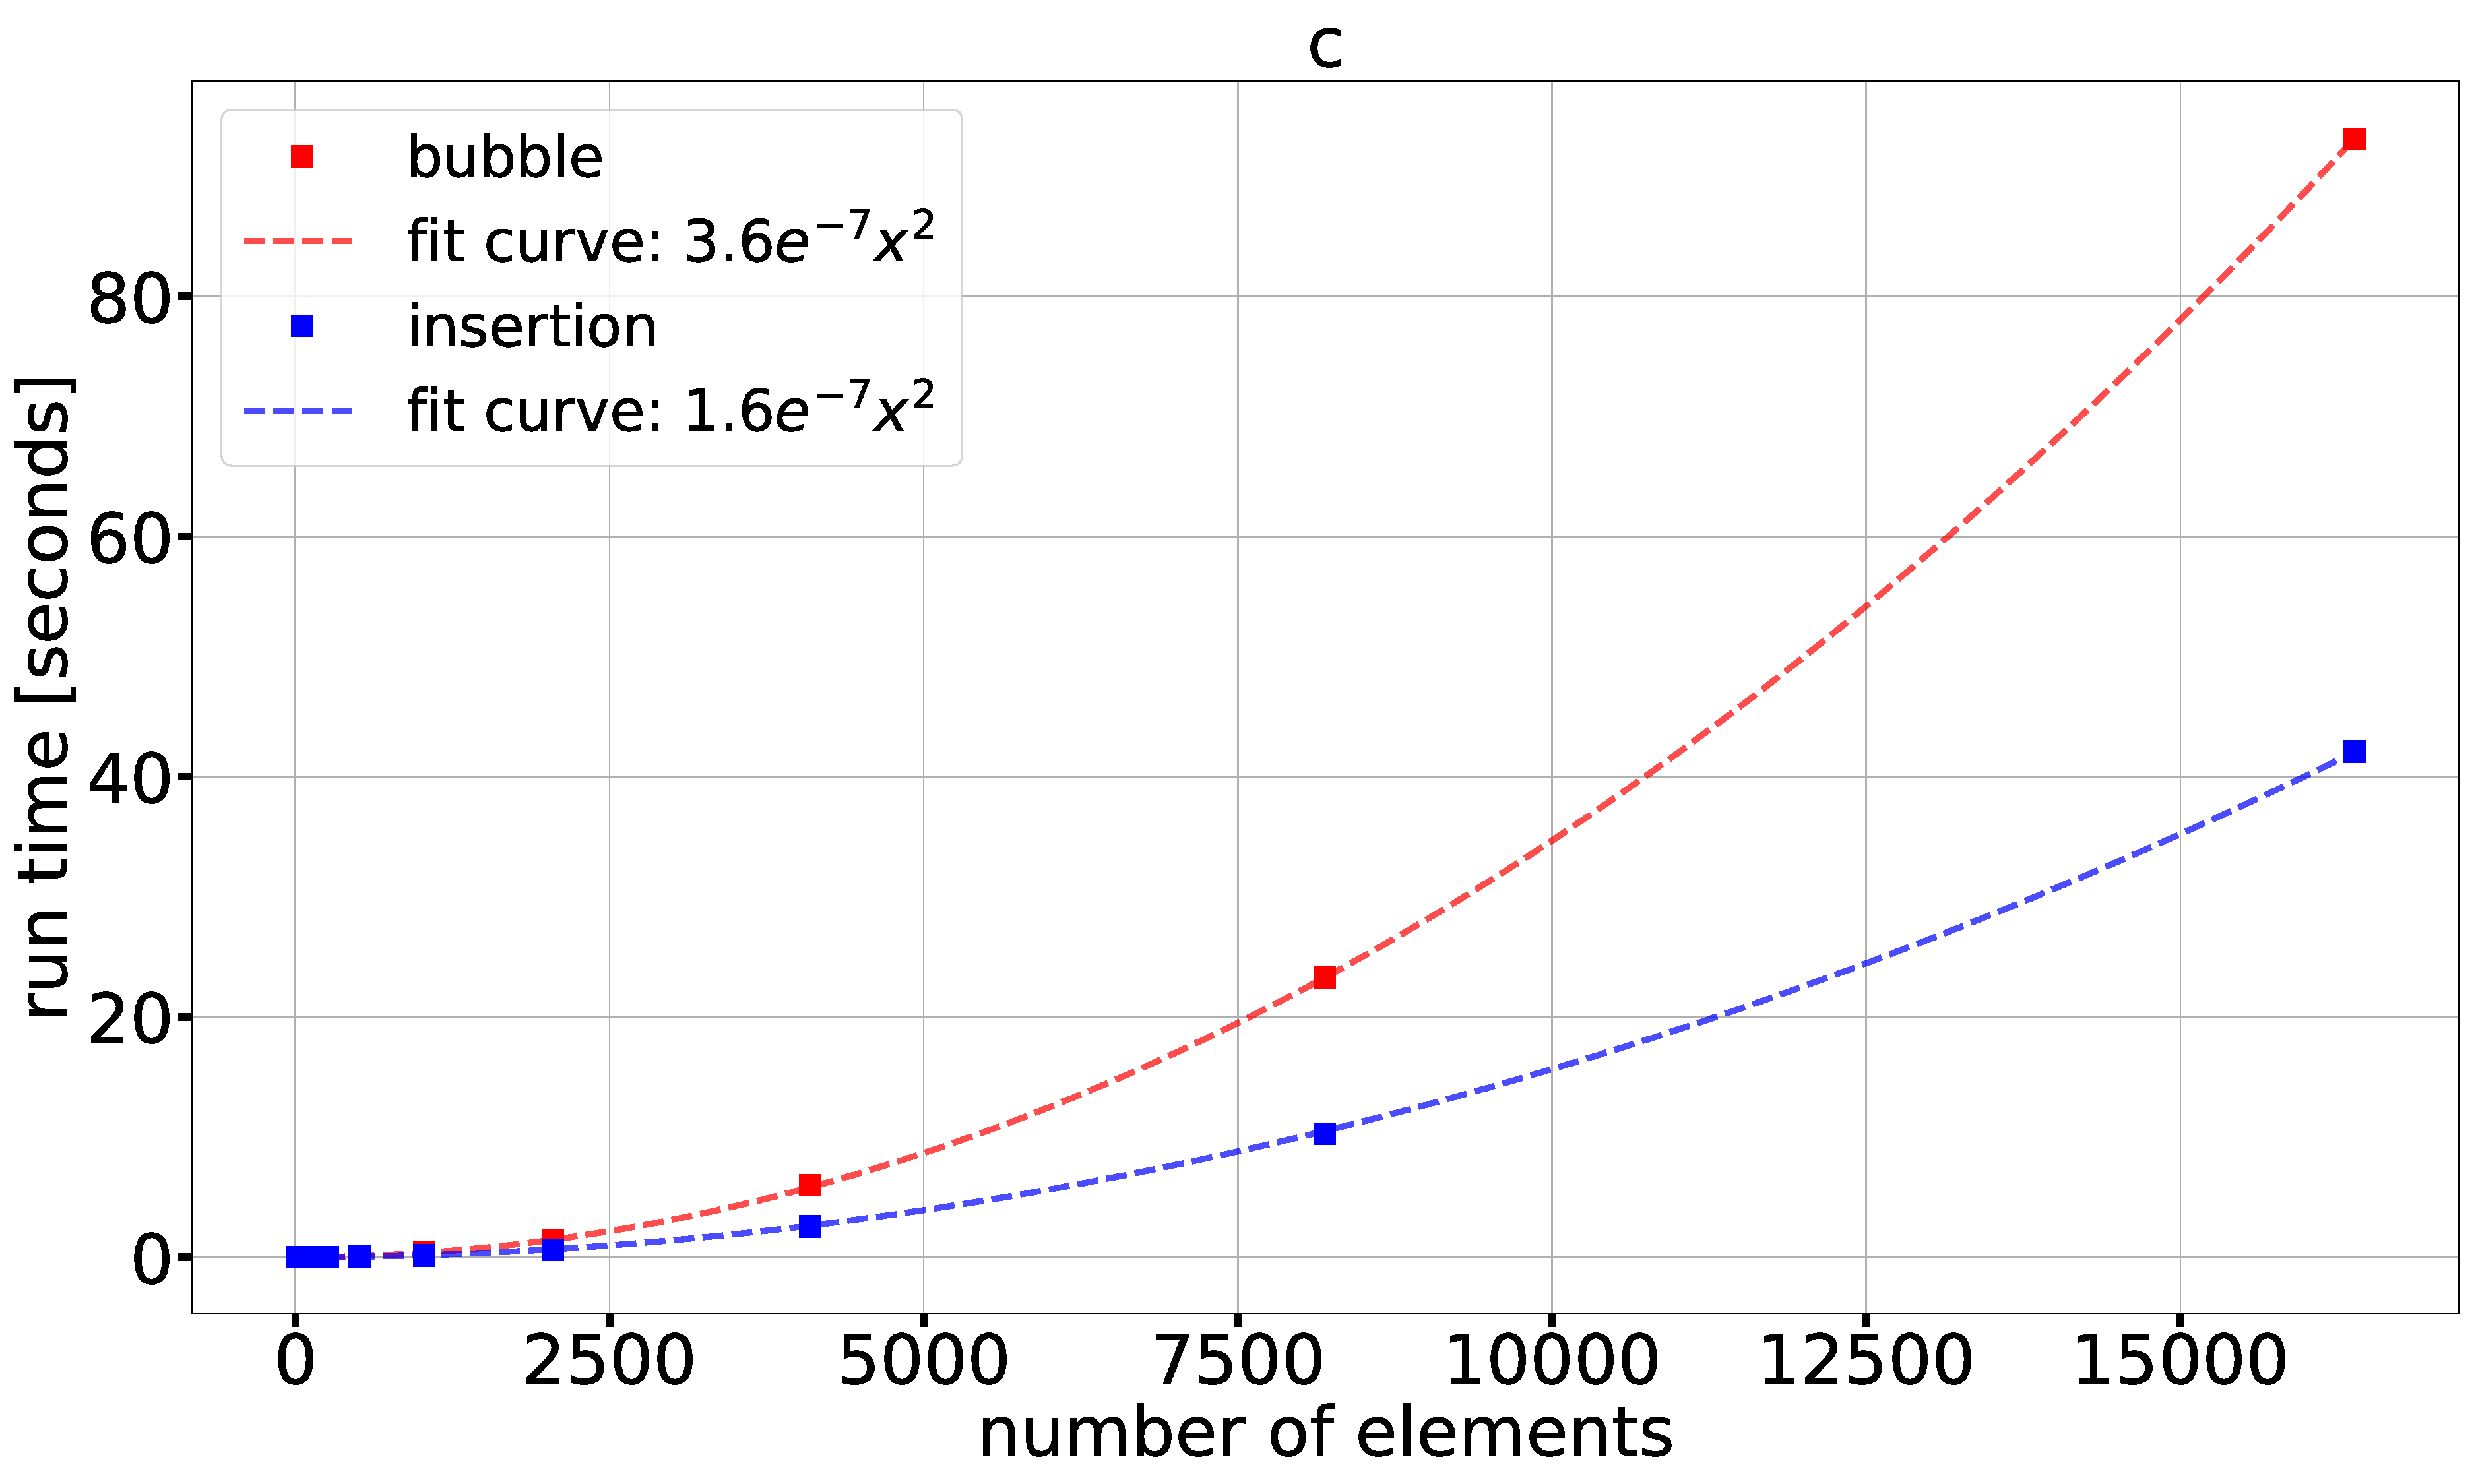
\includegraphics[width=84mm]{../figures/bubble_vs_insertion_reverse.pdf}
  % figure captions below figure
  \caption{Comparison between Bubble-Sort and Insertion-Sort using a)random, b)sorted and c)reversed data. Bubble-Sort shows quadratic run-time on the different permutations. Insertion-Sort shows a linear run-time for sorting the sorted data.}
  \label{fig:quad}
\end{figure}


\subsection{Sub-Quadratic and Combined Sorts}
Figure~\ref{fig:sub_comb} shows the comparison between Quick-Sort, Merge-Sort and Merge-Insertion-Sort for the different data permutation cases. Quick-Sort is approximately $2$ times faster than Merge-Sort. Merge-Insertion-Sort and Merge-Sort have very similar results in sorting the random data. For the data size $16384$, Merge-Insertion-Sort is approximately $15 \%$  faster than Merge-Sort except in the case of reversed data where Merge-Sort is $6 \%$ faster than the Merge-Insertion-Sort. 

\begin{figure}
  \centering
  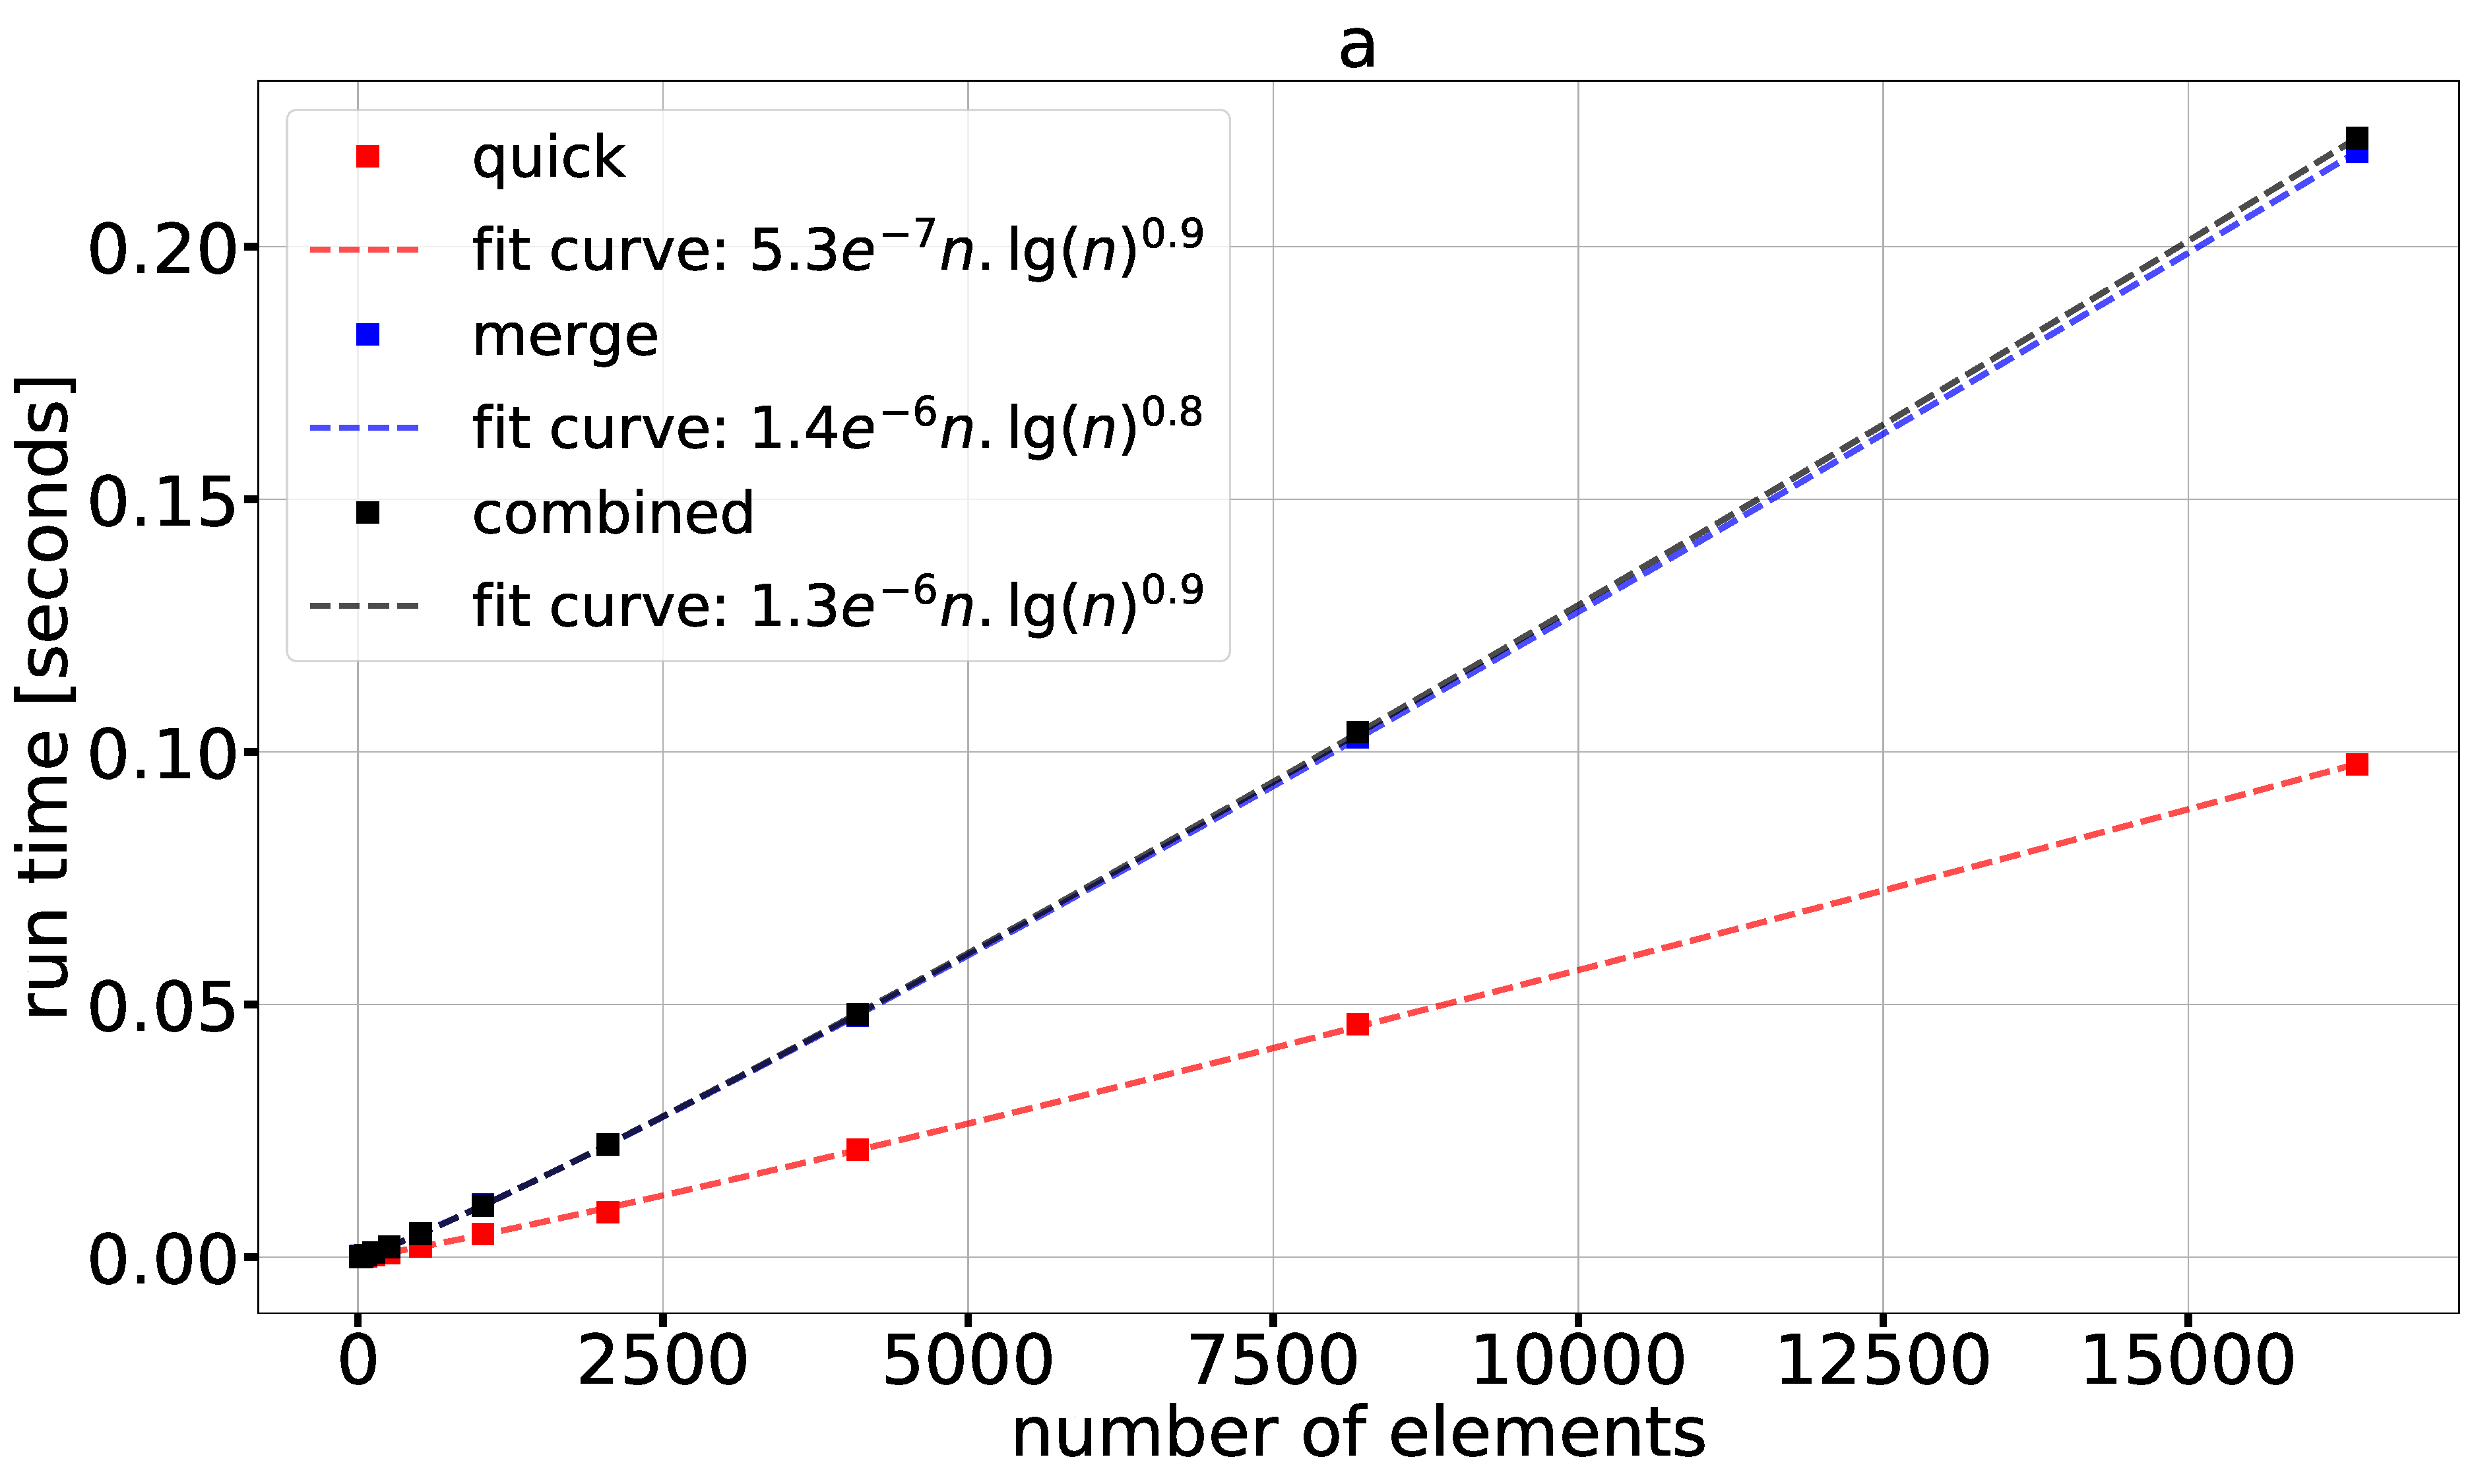
\includegraphics[width=84mm]{../figures/sub_sorts_random.pdf}
  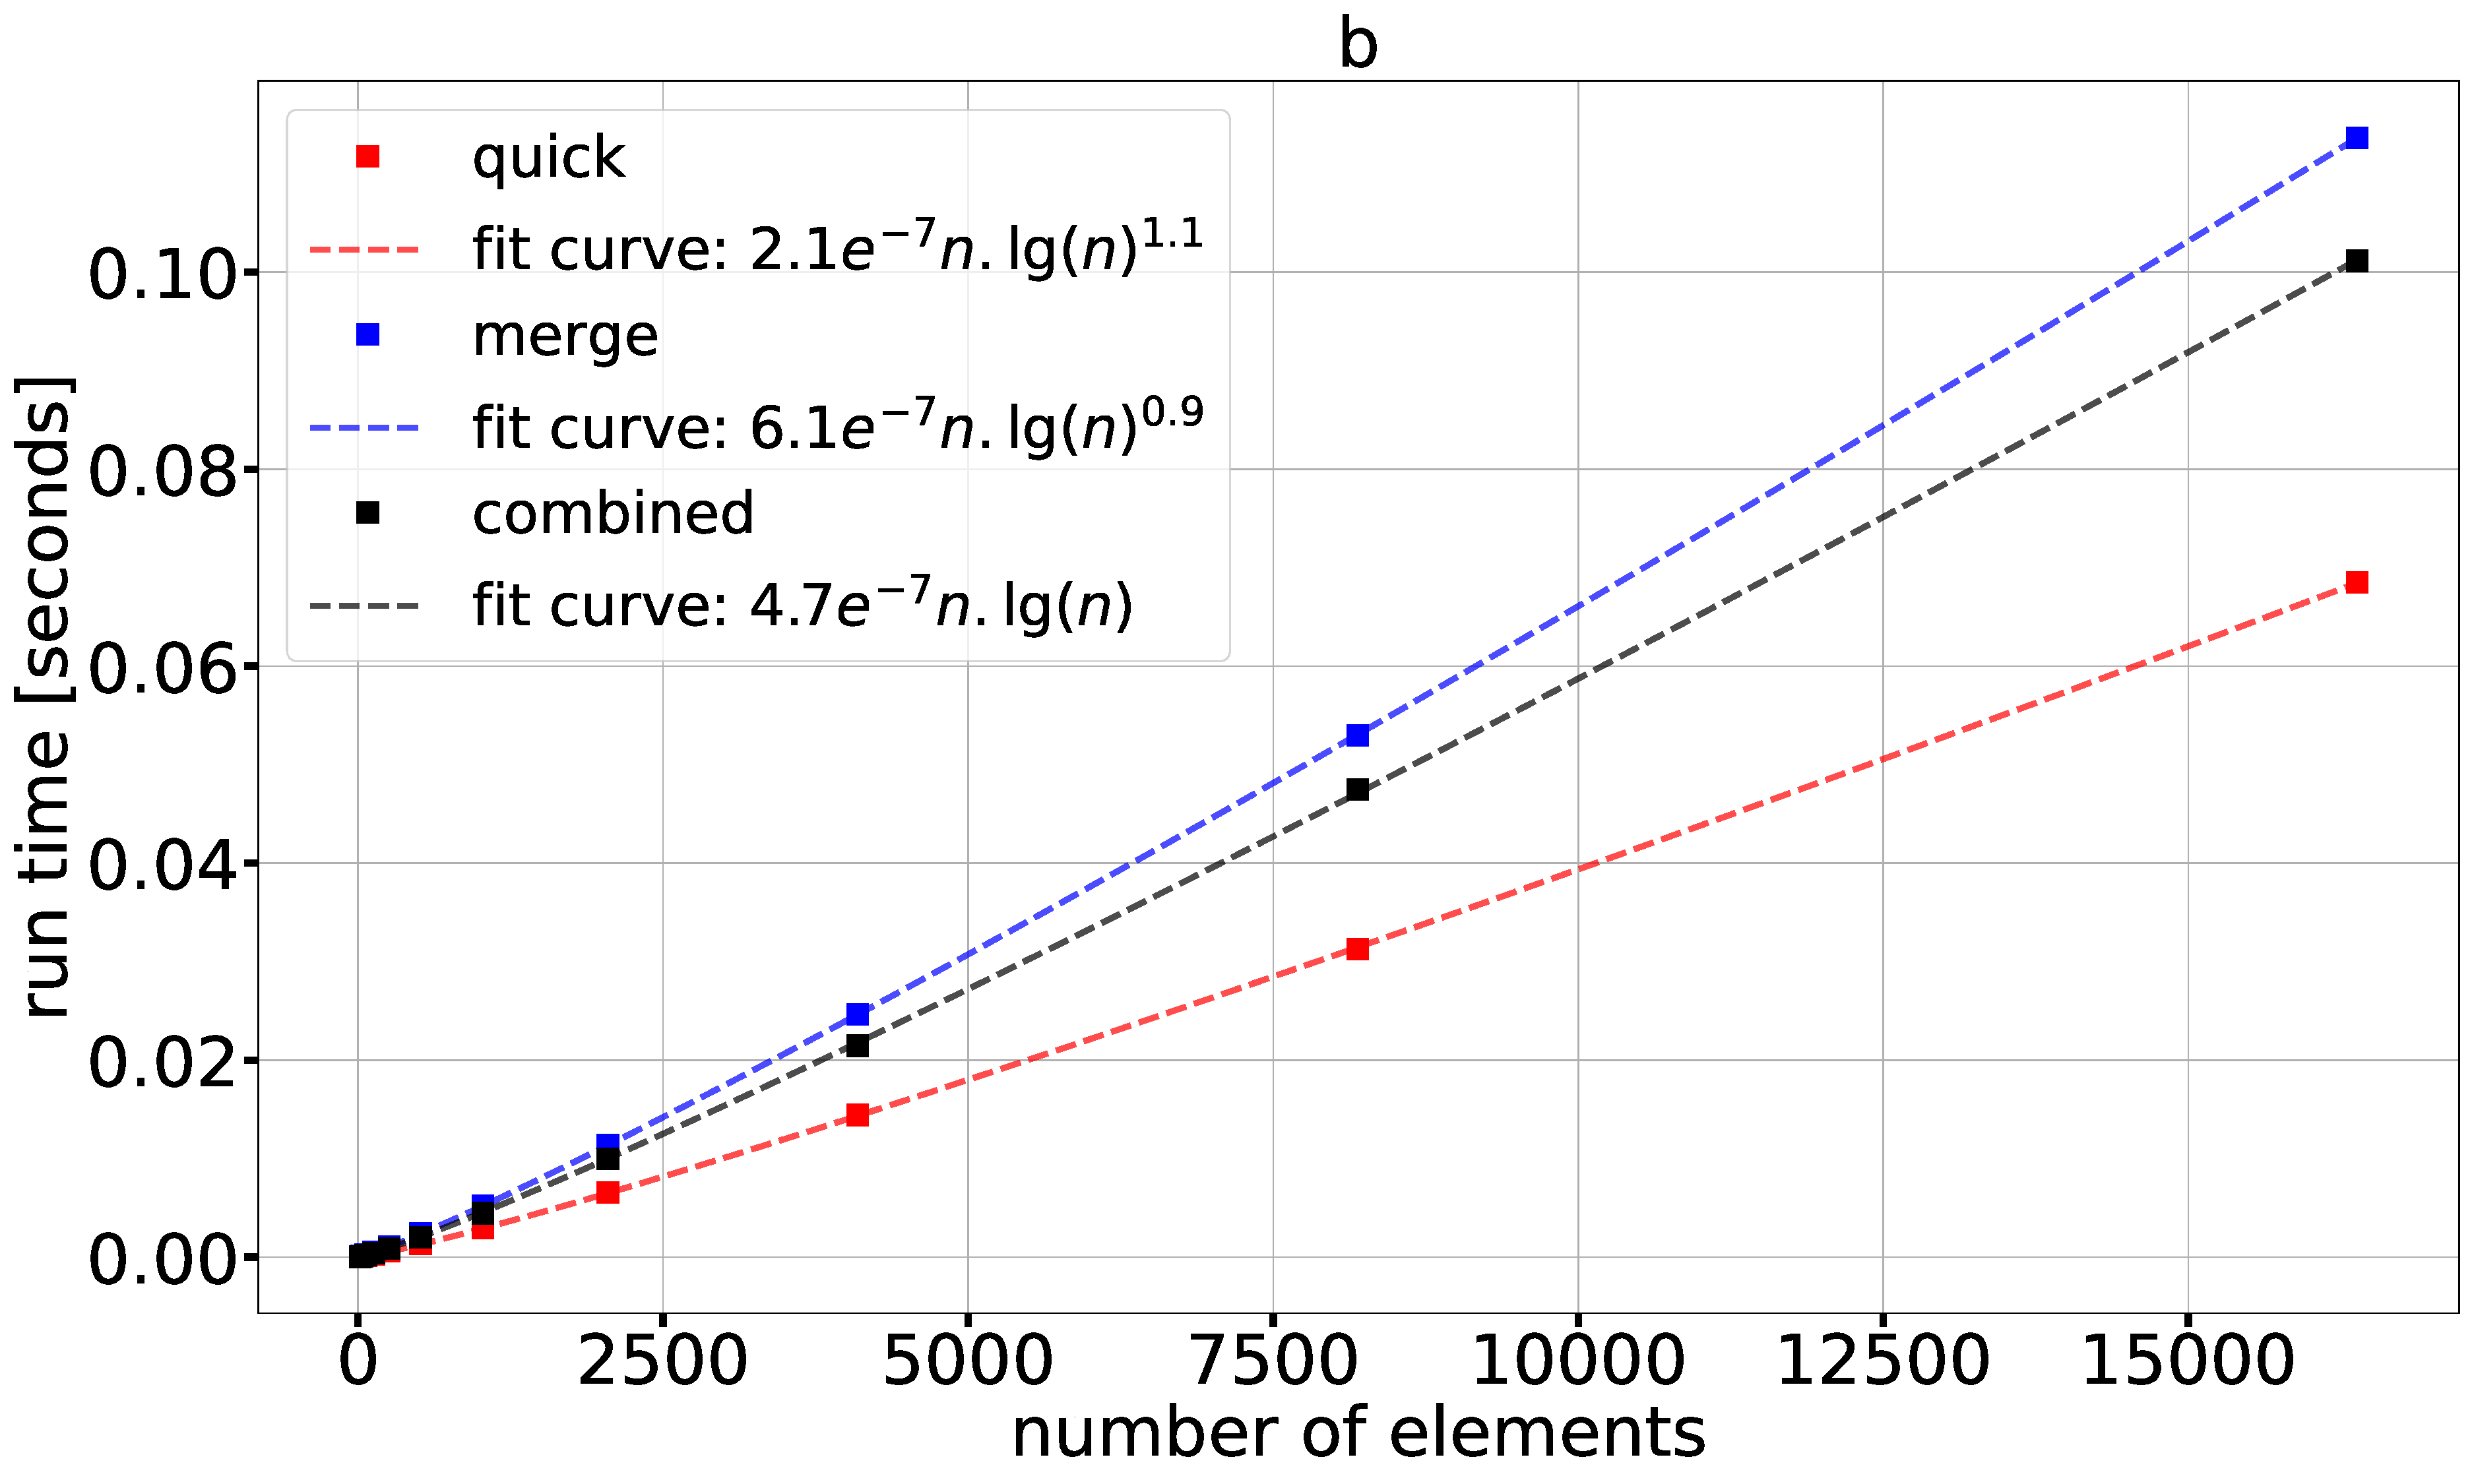
\includegraphics[width=84mm]{../figures/sub_sorts_sorted.pdf}
  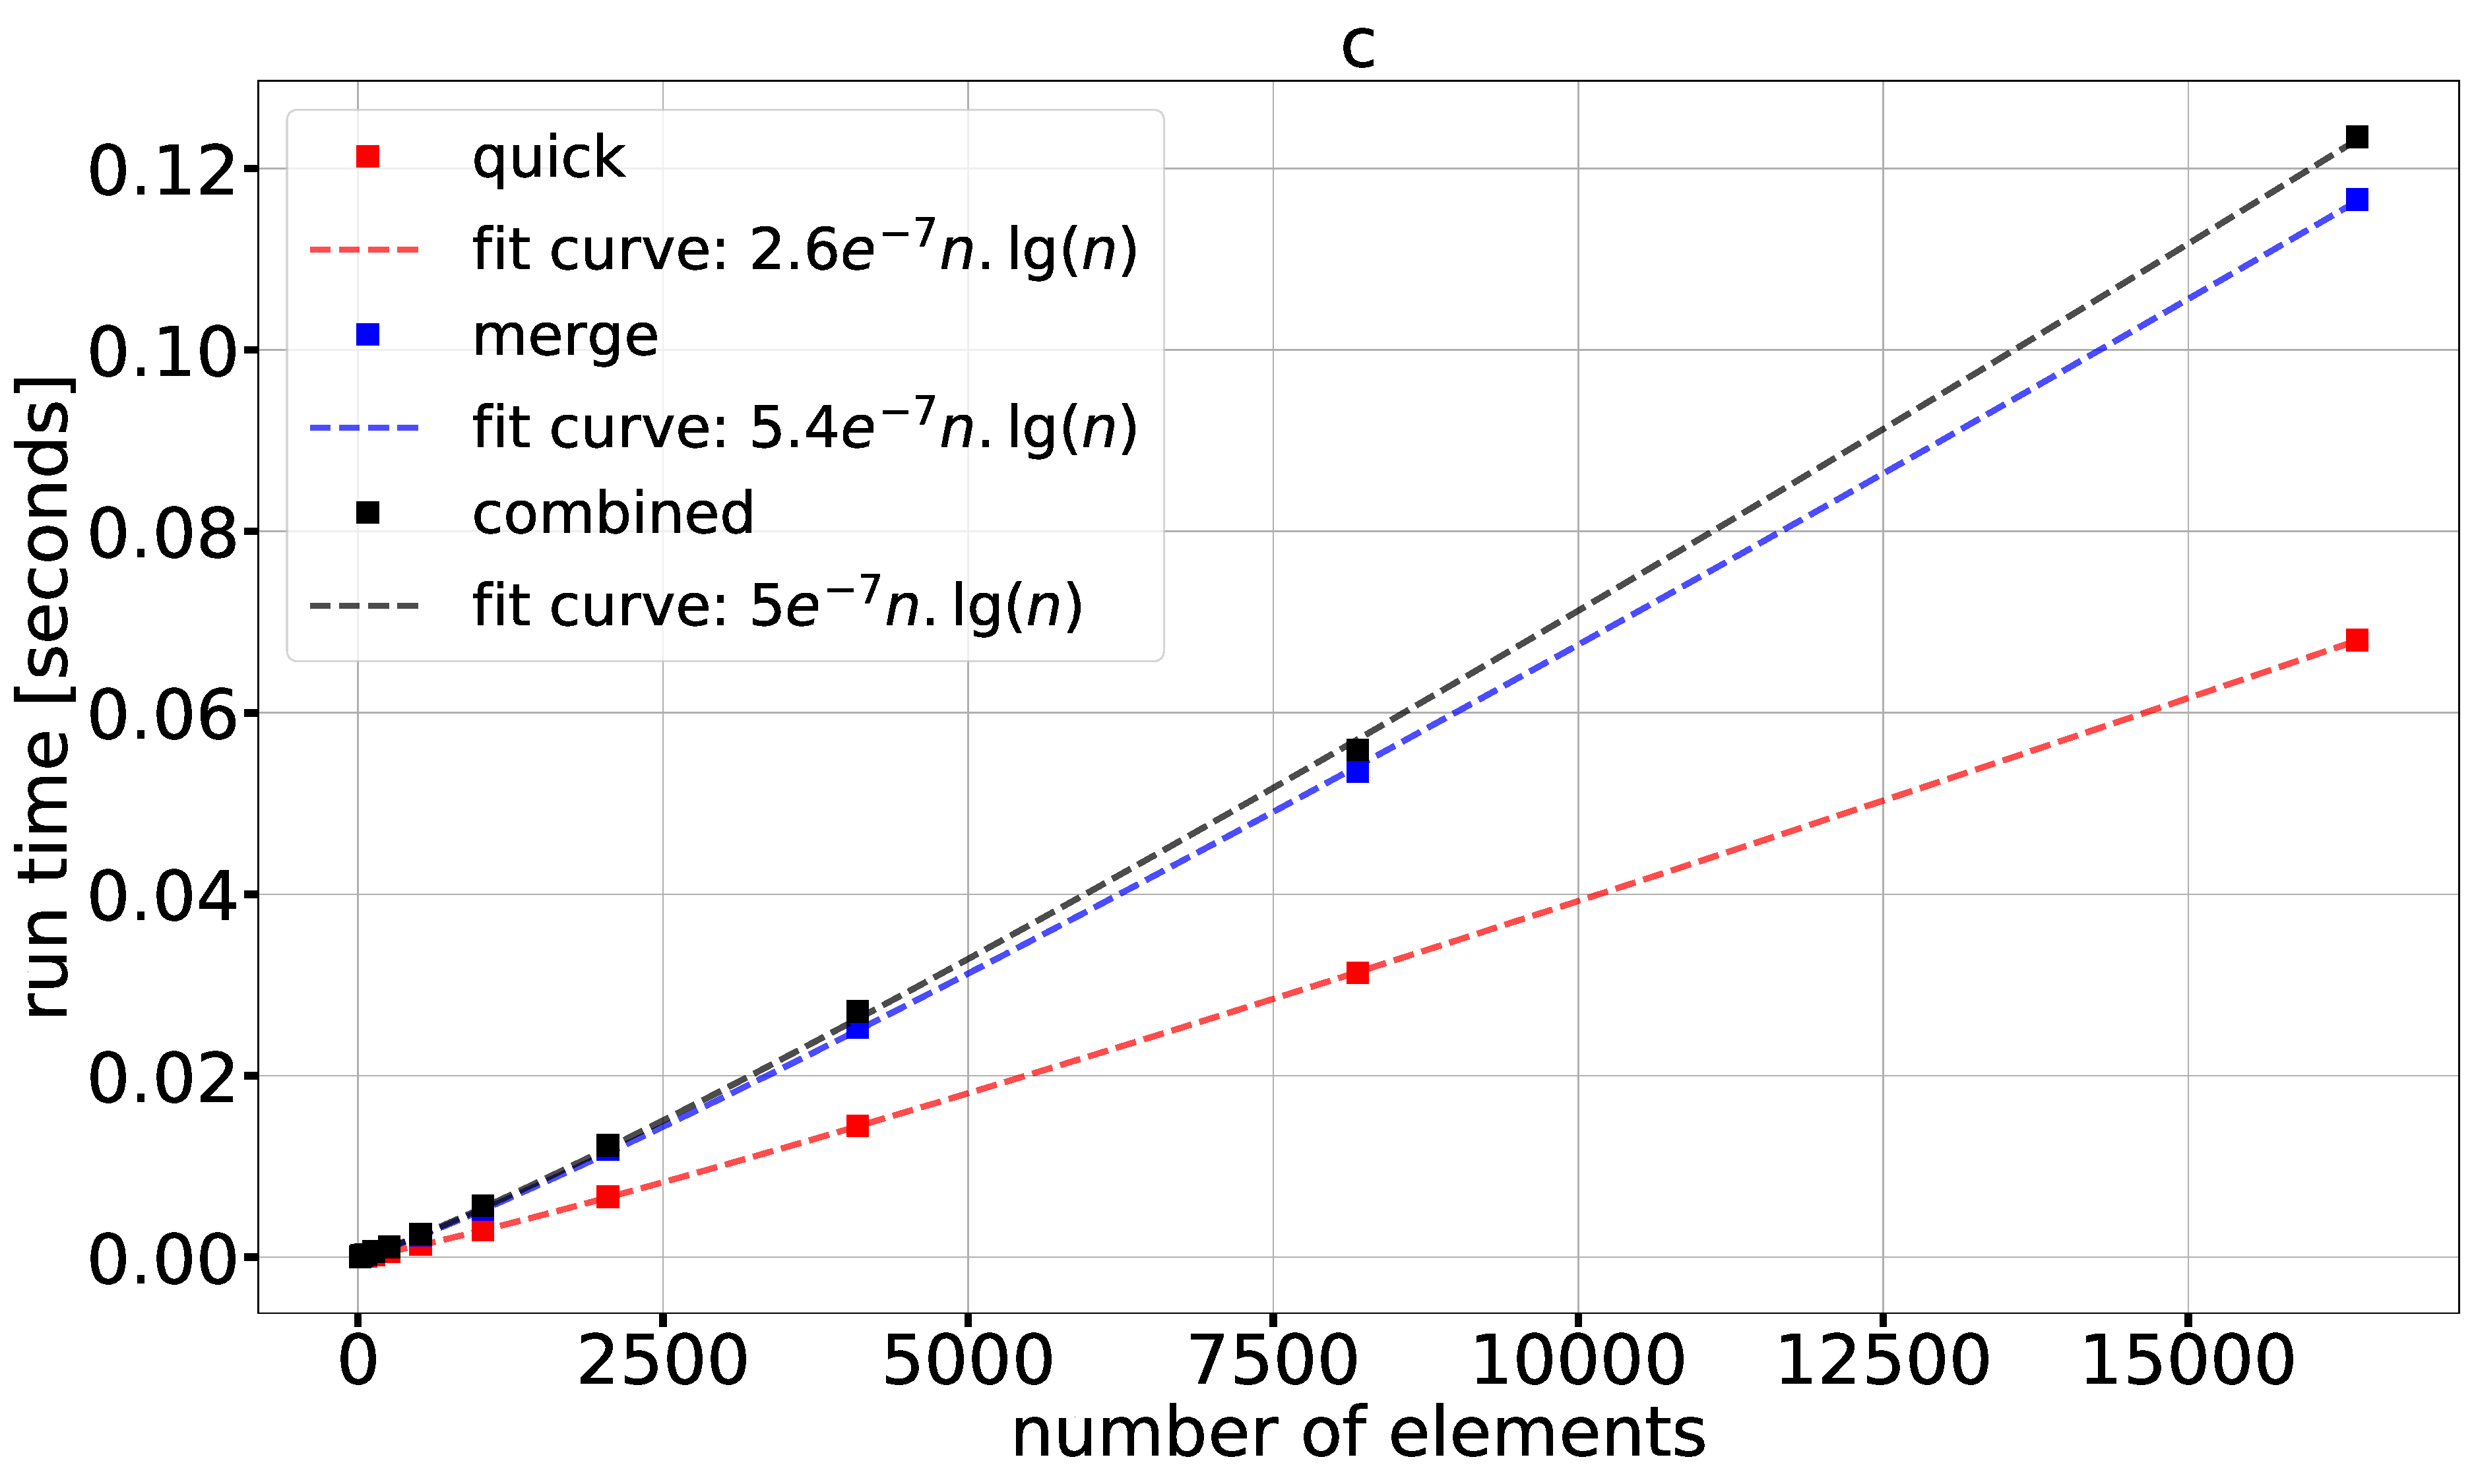
\includegraphics[width=84mm]{../figures/sub_sorts_reverse.pdf}
  % figure captions below figure
  \caption{Comparison between Quick-Sort, Merge-Sort and Merge-Insertion-Sort using a)random, b)sorted and c)reversed data. Notice that Merge-Sort and Merge-Insertion-Sort have identical run-time in sorting random data.}
  \label{fig:sub_comb}
\end{figure}


\subsubsection{Quick-Sort}\label{sec:quick}
\hfill\\
From figure~\ref{fig:quicksort}, sorting random data is only $0.6$ as fast as sorting sorted or reversed data. Figure~\ref{fig:quicksort} show almost very similar results for reversed and sorted data. To further understand these results, we calculated number of executed comparisons within the algorithm for all data permutations and sizes. The results are shown in section.\ref{sec:nr_comparisons}.  

\begin{figure}
  \centering
  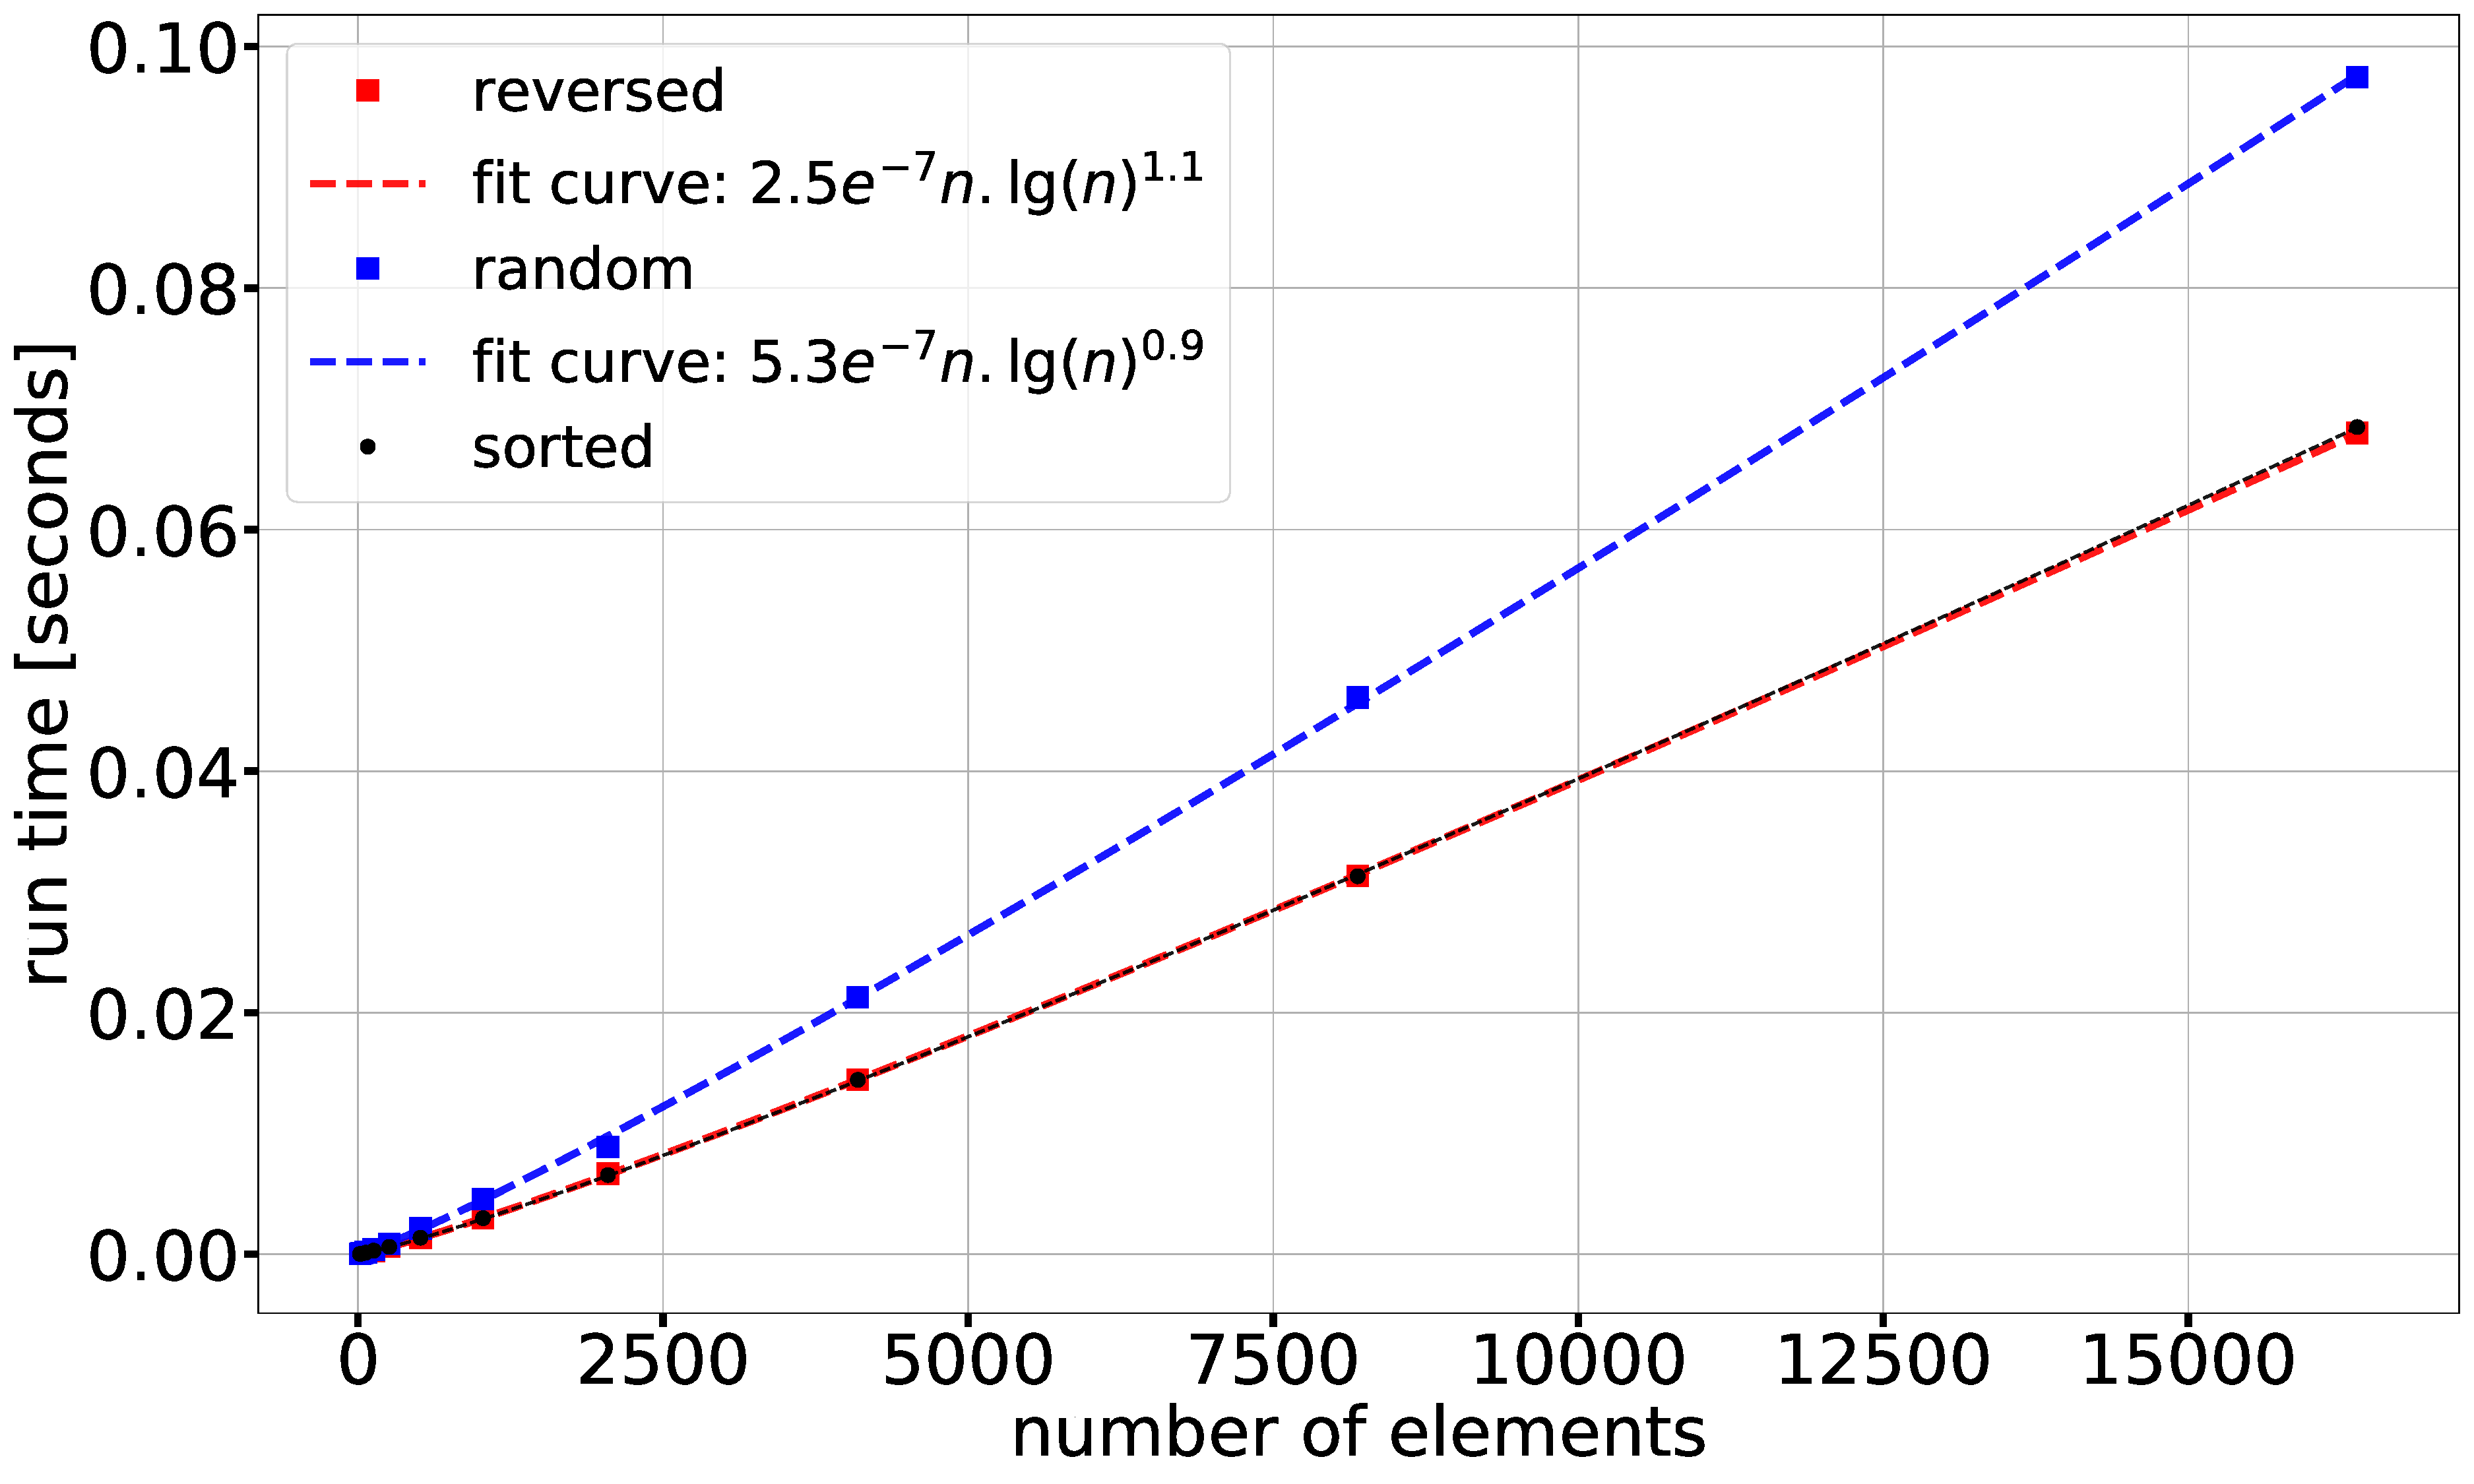
\includegraphics[width=84mm]{../figures/quick_sort.pdf}
  % figure captions below figure
  \caption{Benchmark results for Quick-Sort. Notice the similar run-time for sorting reversed and sorted data. Grey points circles represent the run-time using sorted data which overlap with the run-time using reversed data (red squares). We used the same fit curve for both the reversed and sorted data points.}
  \label{fig:quicksort}
\end{figure}

\subsubsection{Merge-Sort}\label{sec:merge}
\hfill\\
In Merge-Sort, it is clear that sorting already sorted data takes very similar run-time as sorting reversed data while random data takes longer time as shown in figure~\ref{fig:merge}. From the results, sorting already sorted or reversed data is $2$ times faster than sorting random data.

\begin{figure}
  \centering
  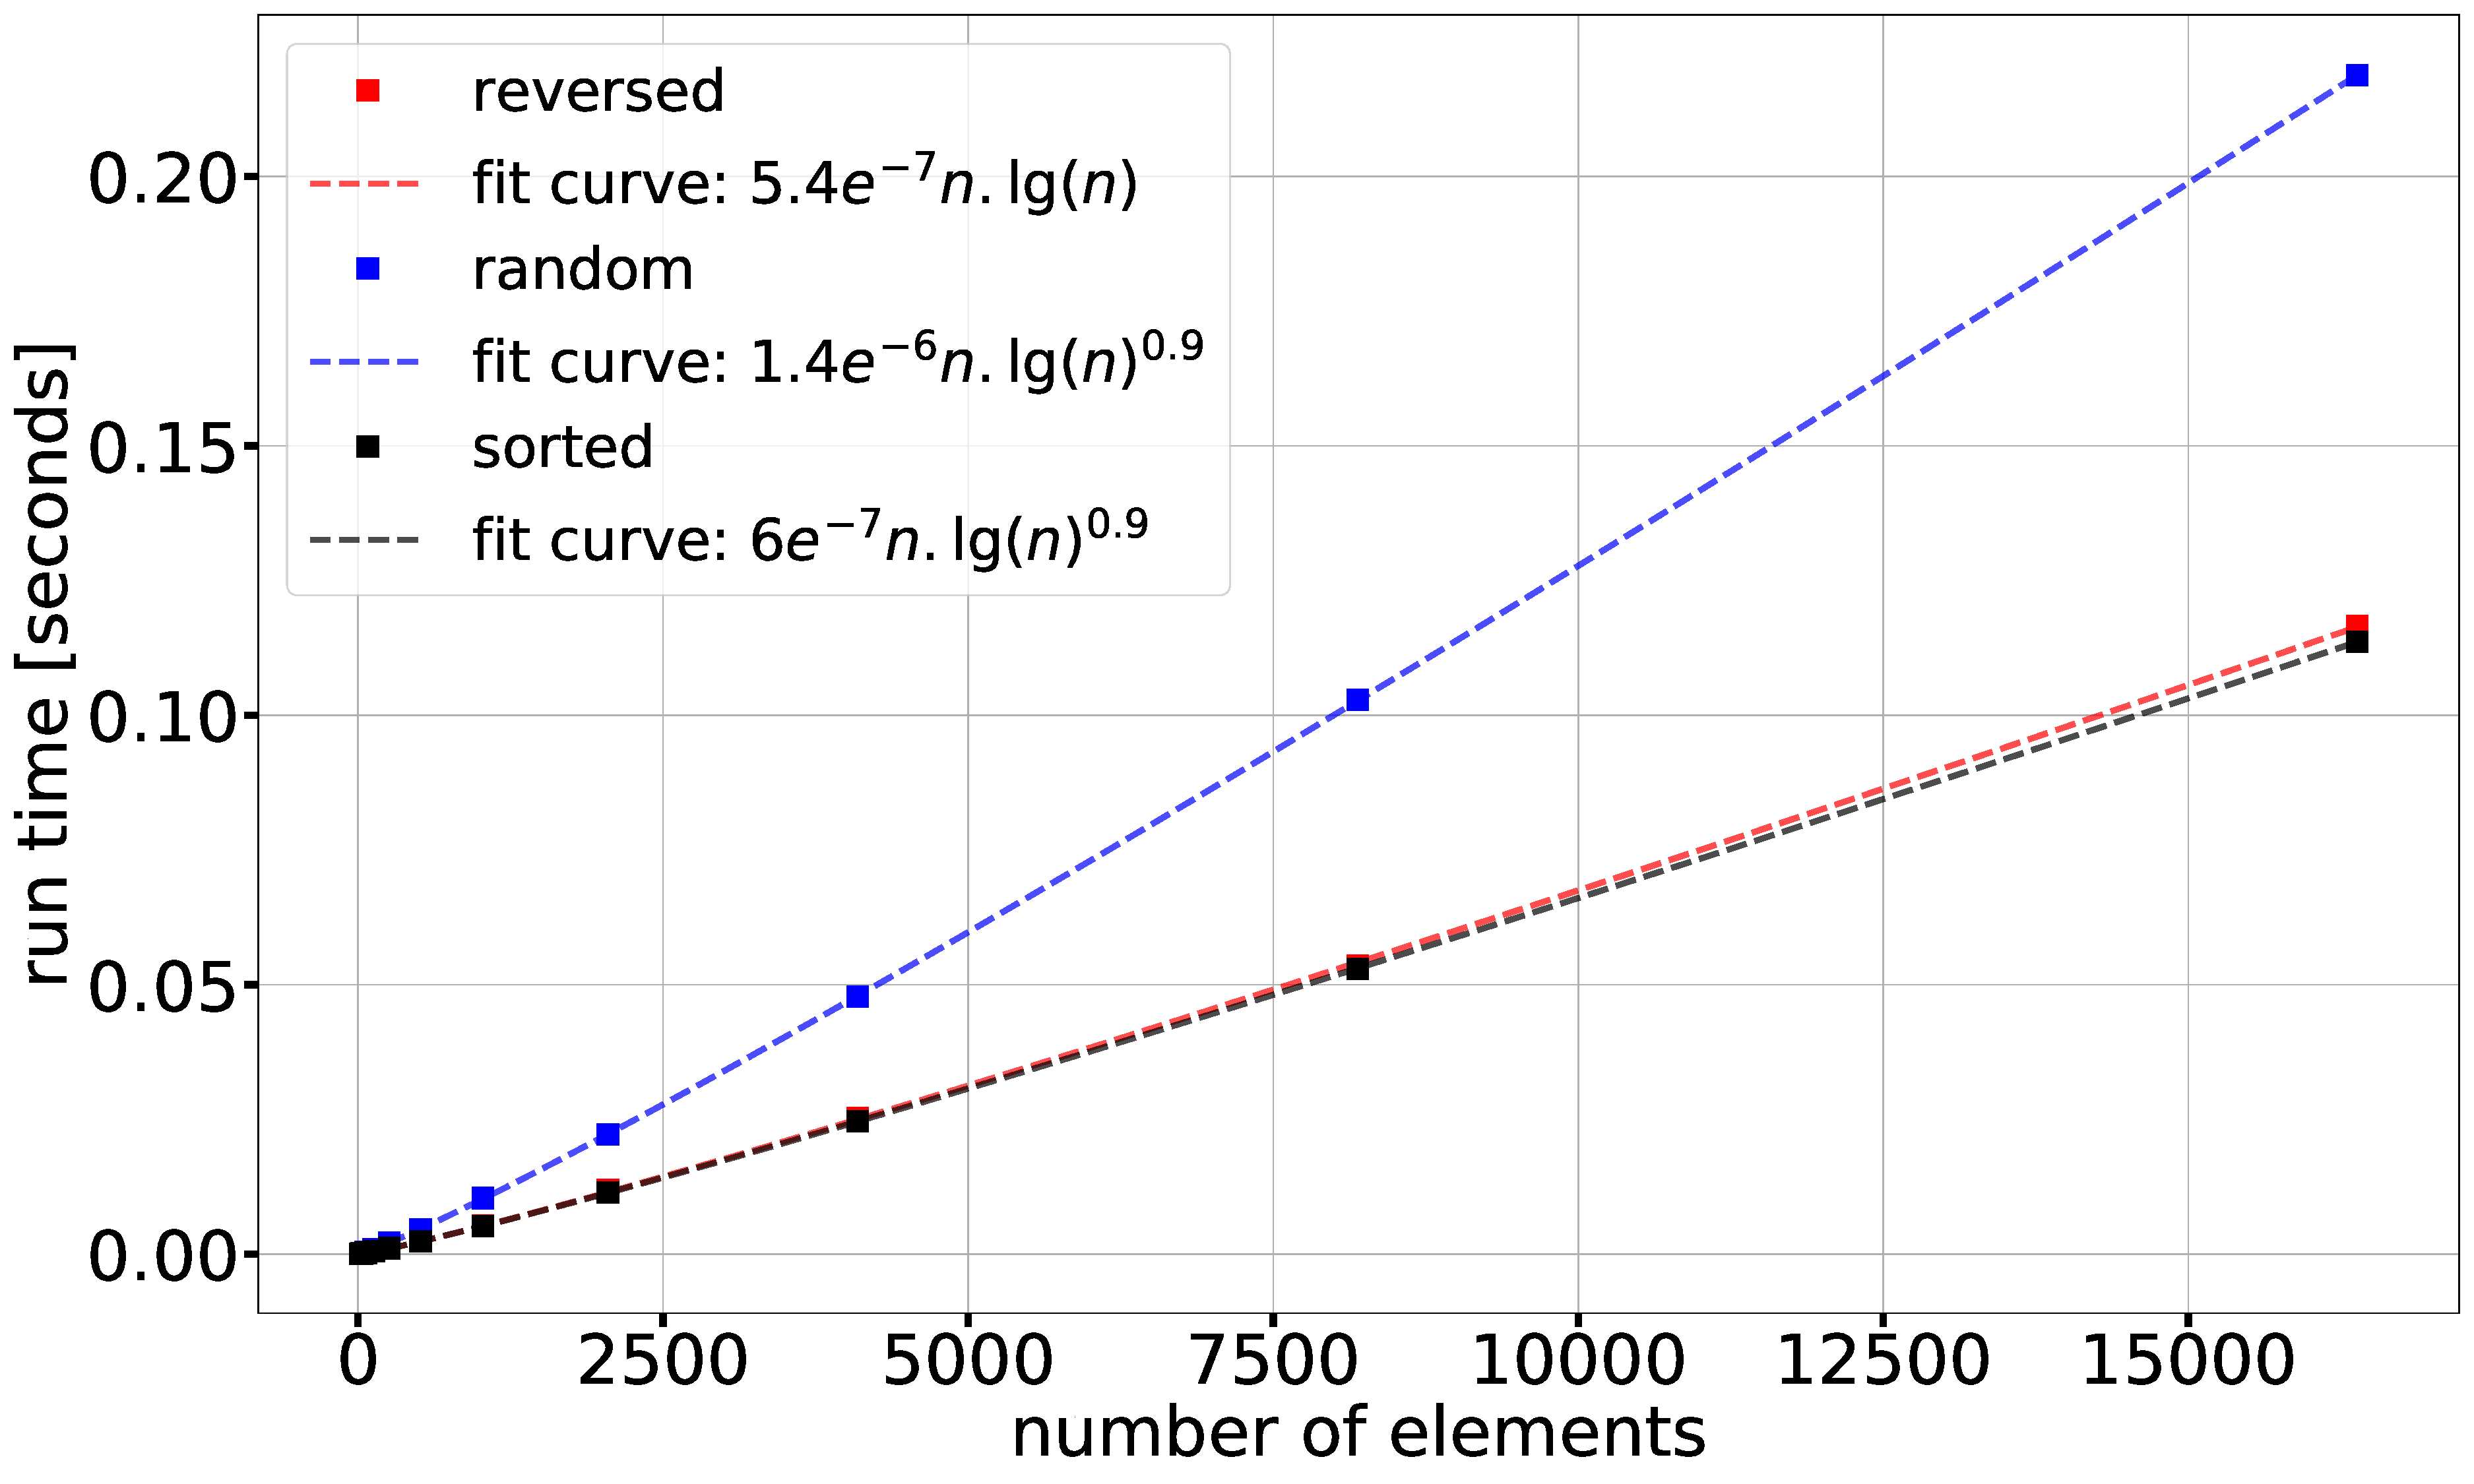
\includegraphics[width=84mm]{../figures/merge_sort.pdf}
  % figure captions below figure
  \caption{Benchmark results for Merge-Sort. Notice the similar run-time for sorting reversed and sorted data.}
  \label{fig:merge}
\end{figure}
\subsubsection{Merge-Insertion-Sort}\label{sec:combined}
\hfill\\
Figure~\ref{fig:comb} shows that sorting reversed data is $2$ times faster than sorting random data. Merge-Insertion-Sort does not show similar results for sorting sorted data and sorting reversed data unlike Merge-Sort and Quick-Sort. 

\begin{figure}
  \centering
  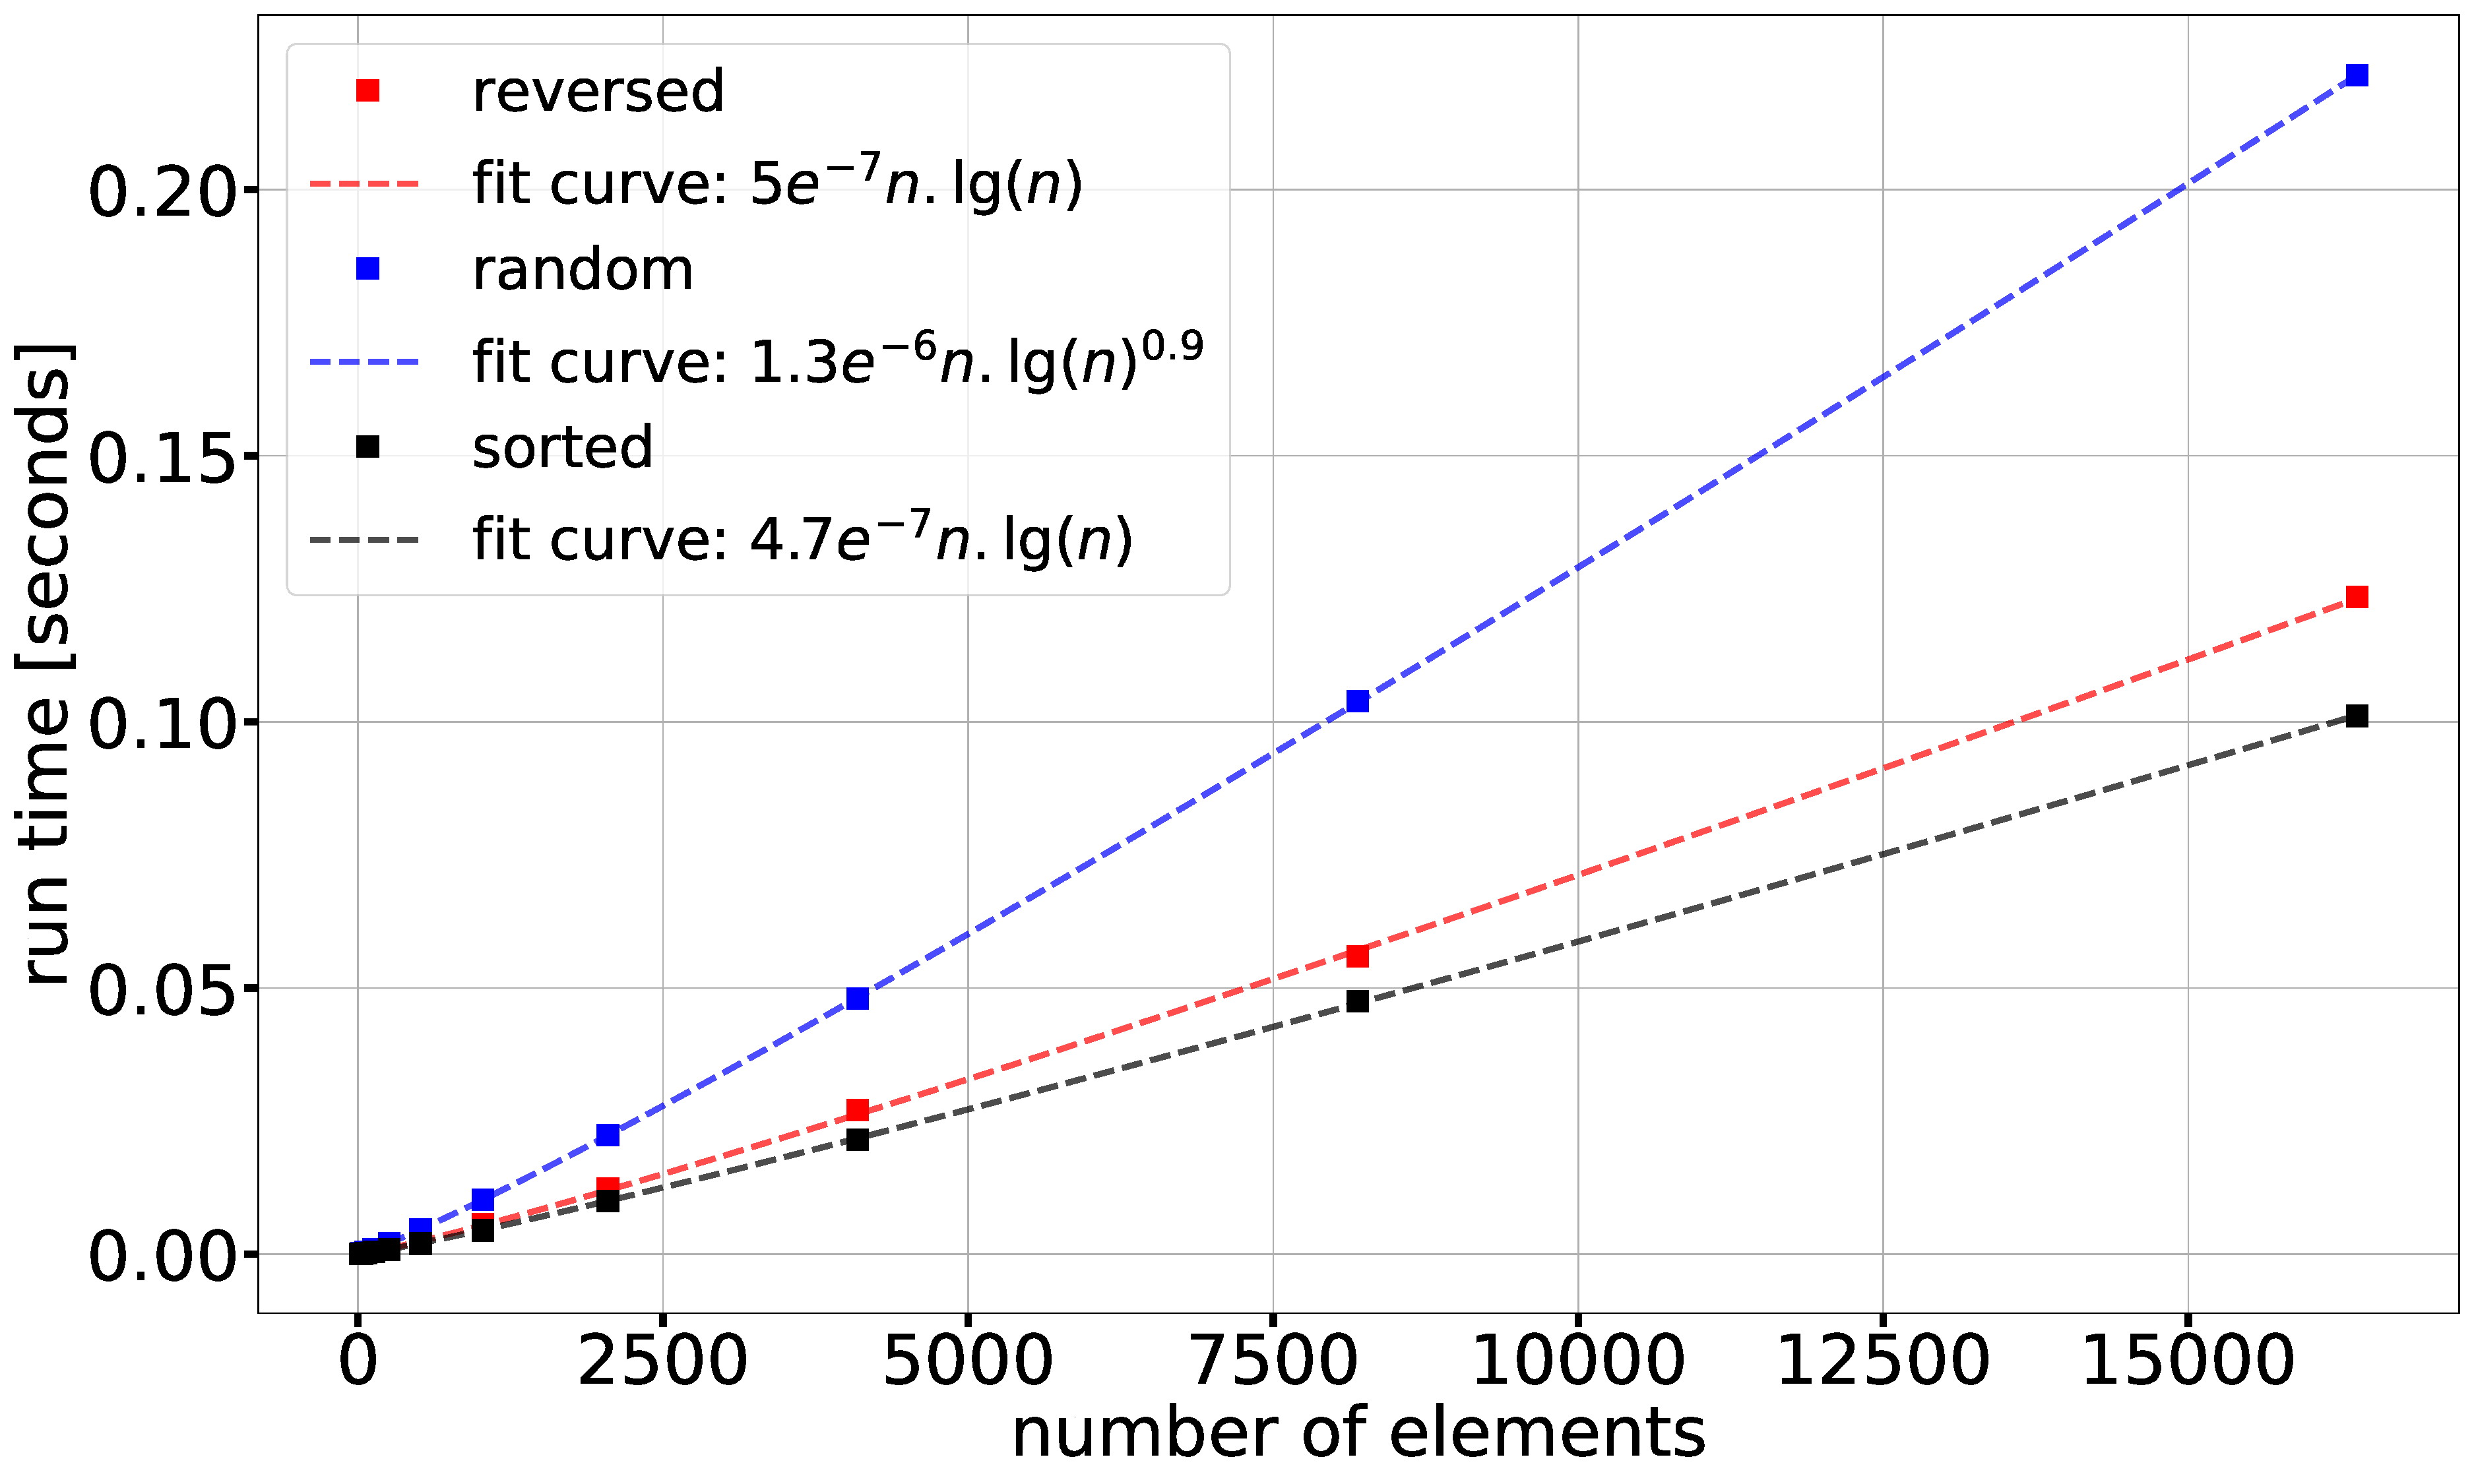
\includegraphics[width=84mm]{../figures/combined_sort.pdf}
  % figure captions below figure
  \caption{Benchmark results for Merge-Insertion-Sort}
  \label{fig:comb}
\end{figure}

\subsection{Built-in Sorts}\label{sec:builtin}
Python-Sort also shows the noticed observation of Merge-Sort that performances are almost identical for sorted and reversed data which is noticed from figure~\ref{fig:py}. Using Python-Sort to sort sorted and reversed data is almost $12$ times faster than sorting random data. Also, Python-Sort is $10$ times faster than our implementation Merge-Insertion-Sort.
\hfill\\
Application of Numpy-Sort on random data is approximately $2$ times faster than application of Numpy-Sort on sorted data as shown in figure ~\ref{fig:np}. Also, it is noticed that Numpy-Sort is almost $10$ times faster in sorting the random data than Python-Sort in sorting the random data.
\begin{figure}
  \centering
  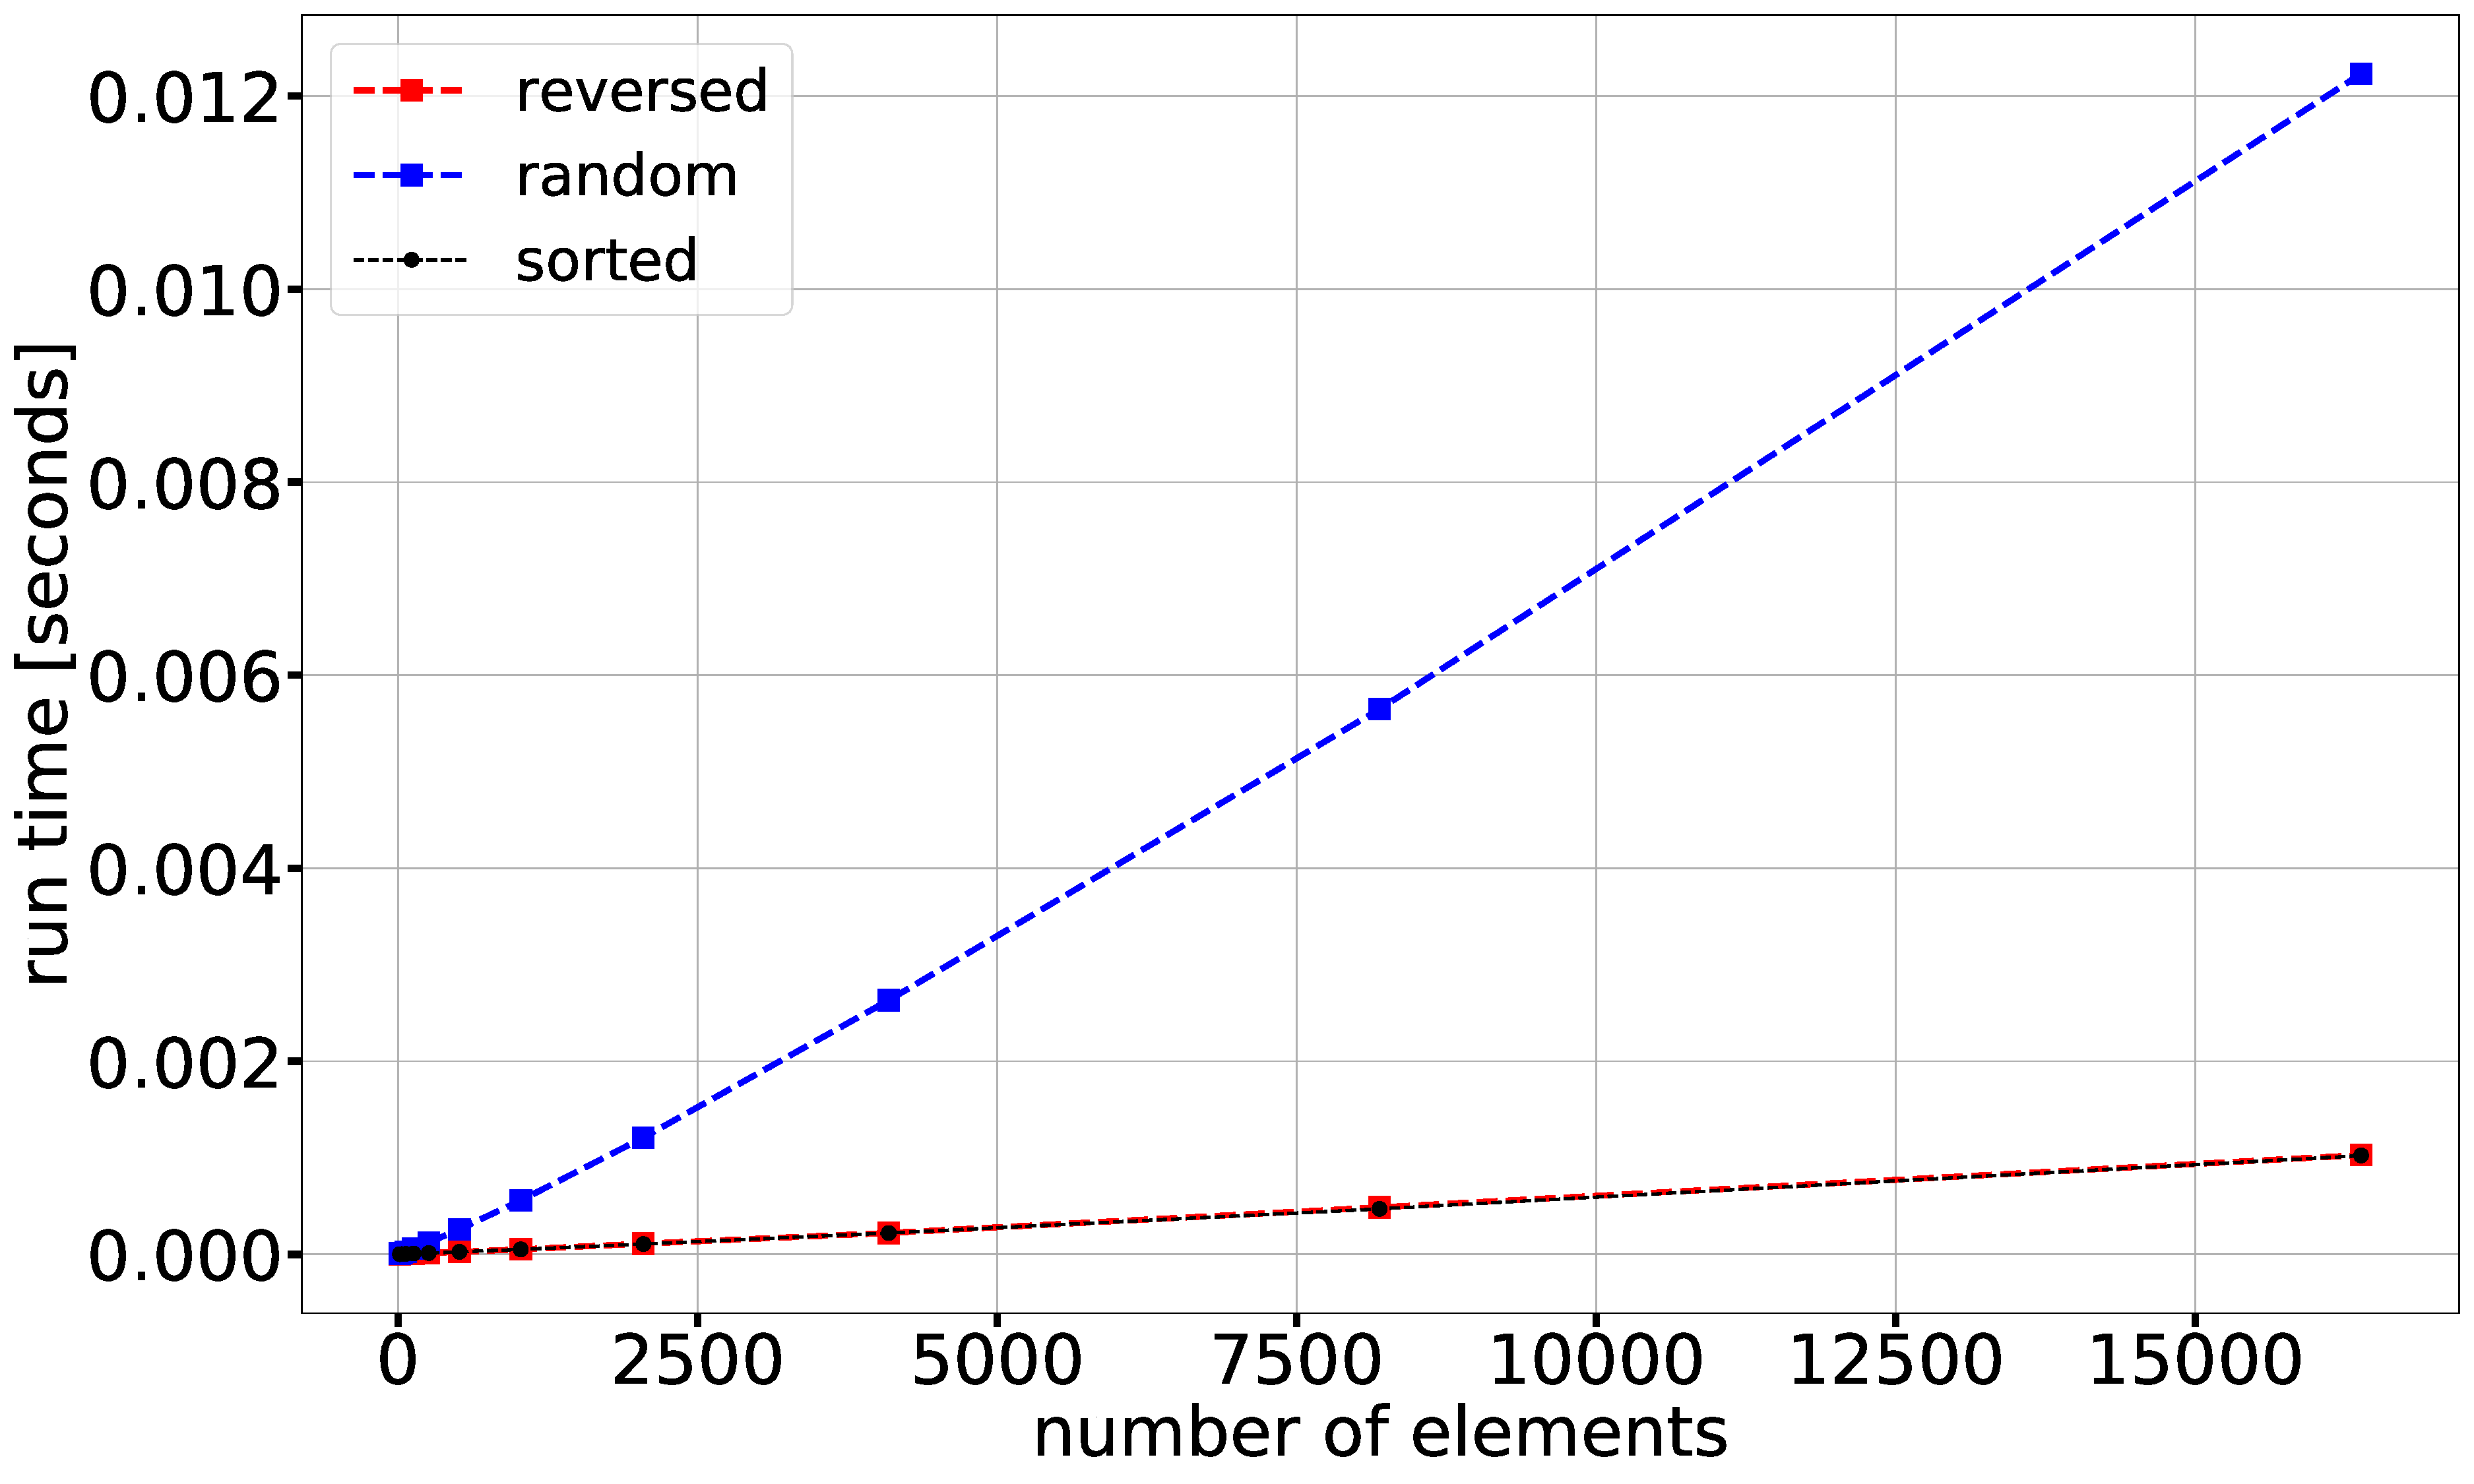
\includegraphics[width=84mm]{../figures/py_sort.pdf}
  % figure captions below figure
  \caption{Benchmark results for Python built-in sort on sorted and reversed data. Notice the identical run-time for sorting reversed and sorted data. Grey points circles represent the run-time benchmark using sorted data which overlap with the run-time benchmark using reversed data.}
  \label{fig:py}
\end{figure}

\begin{figure}
  \centering
  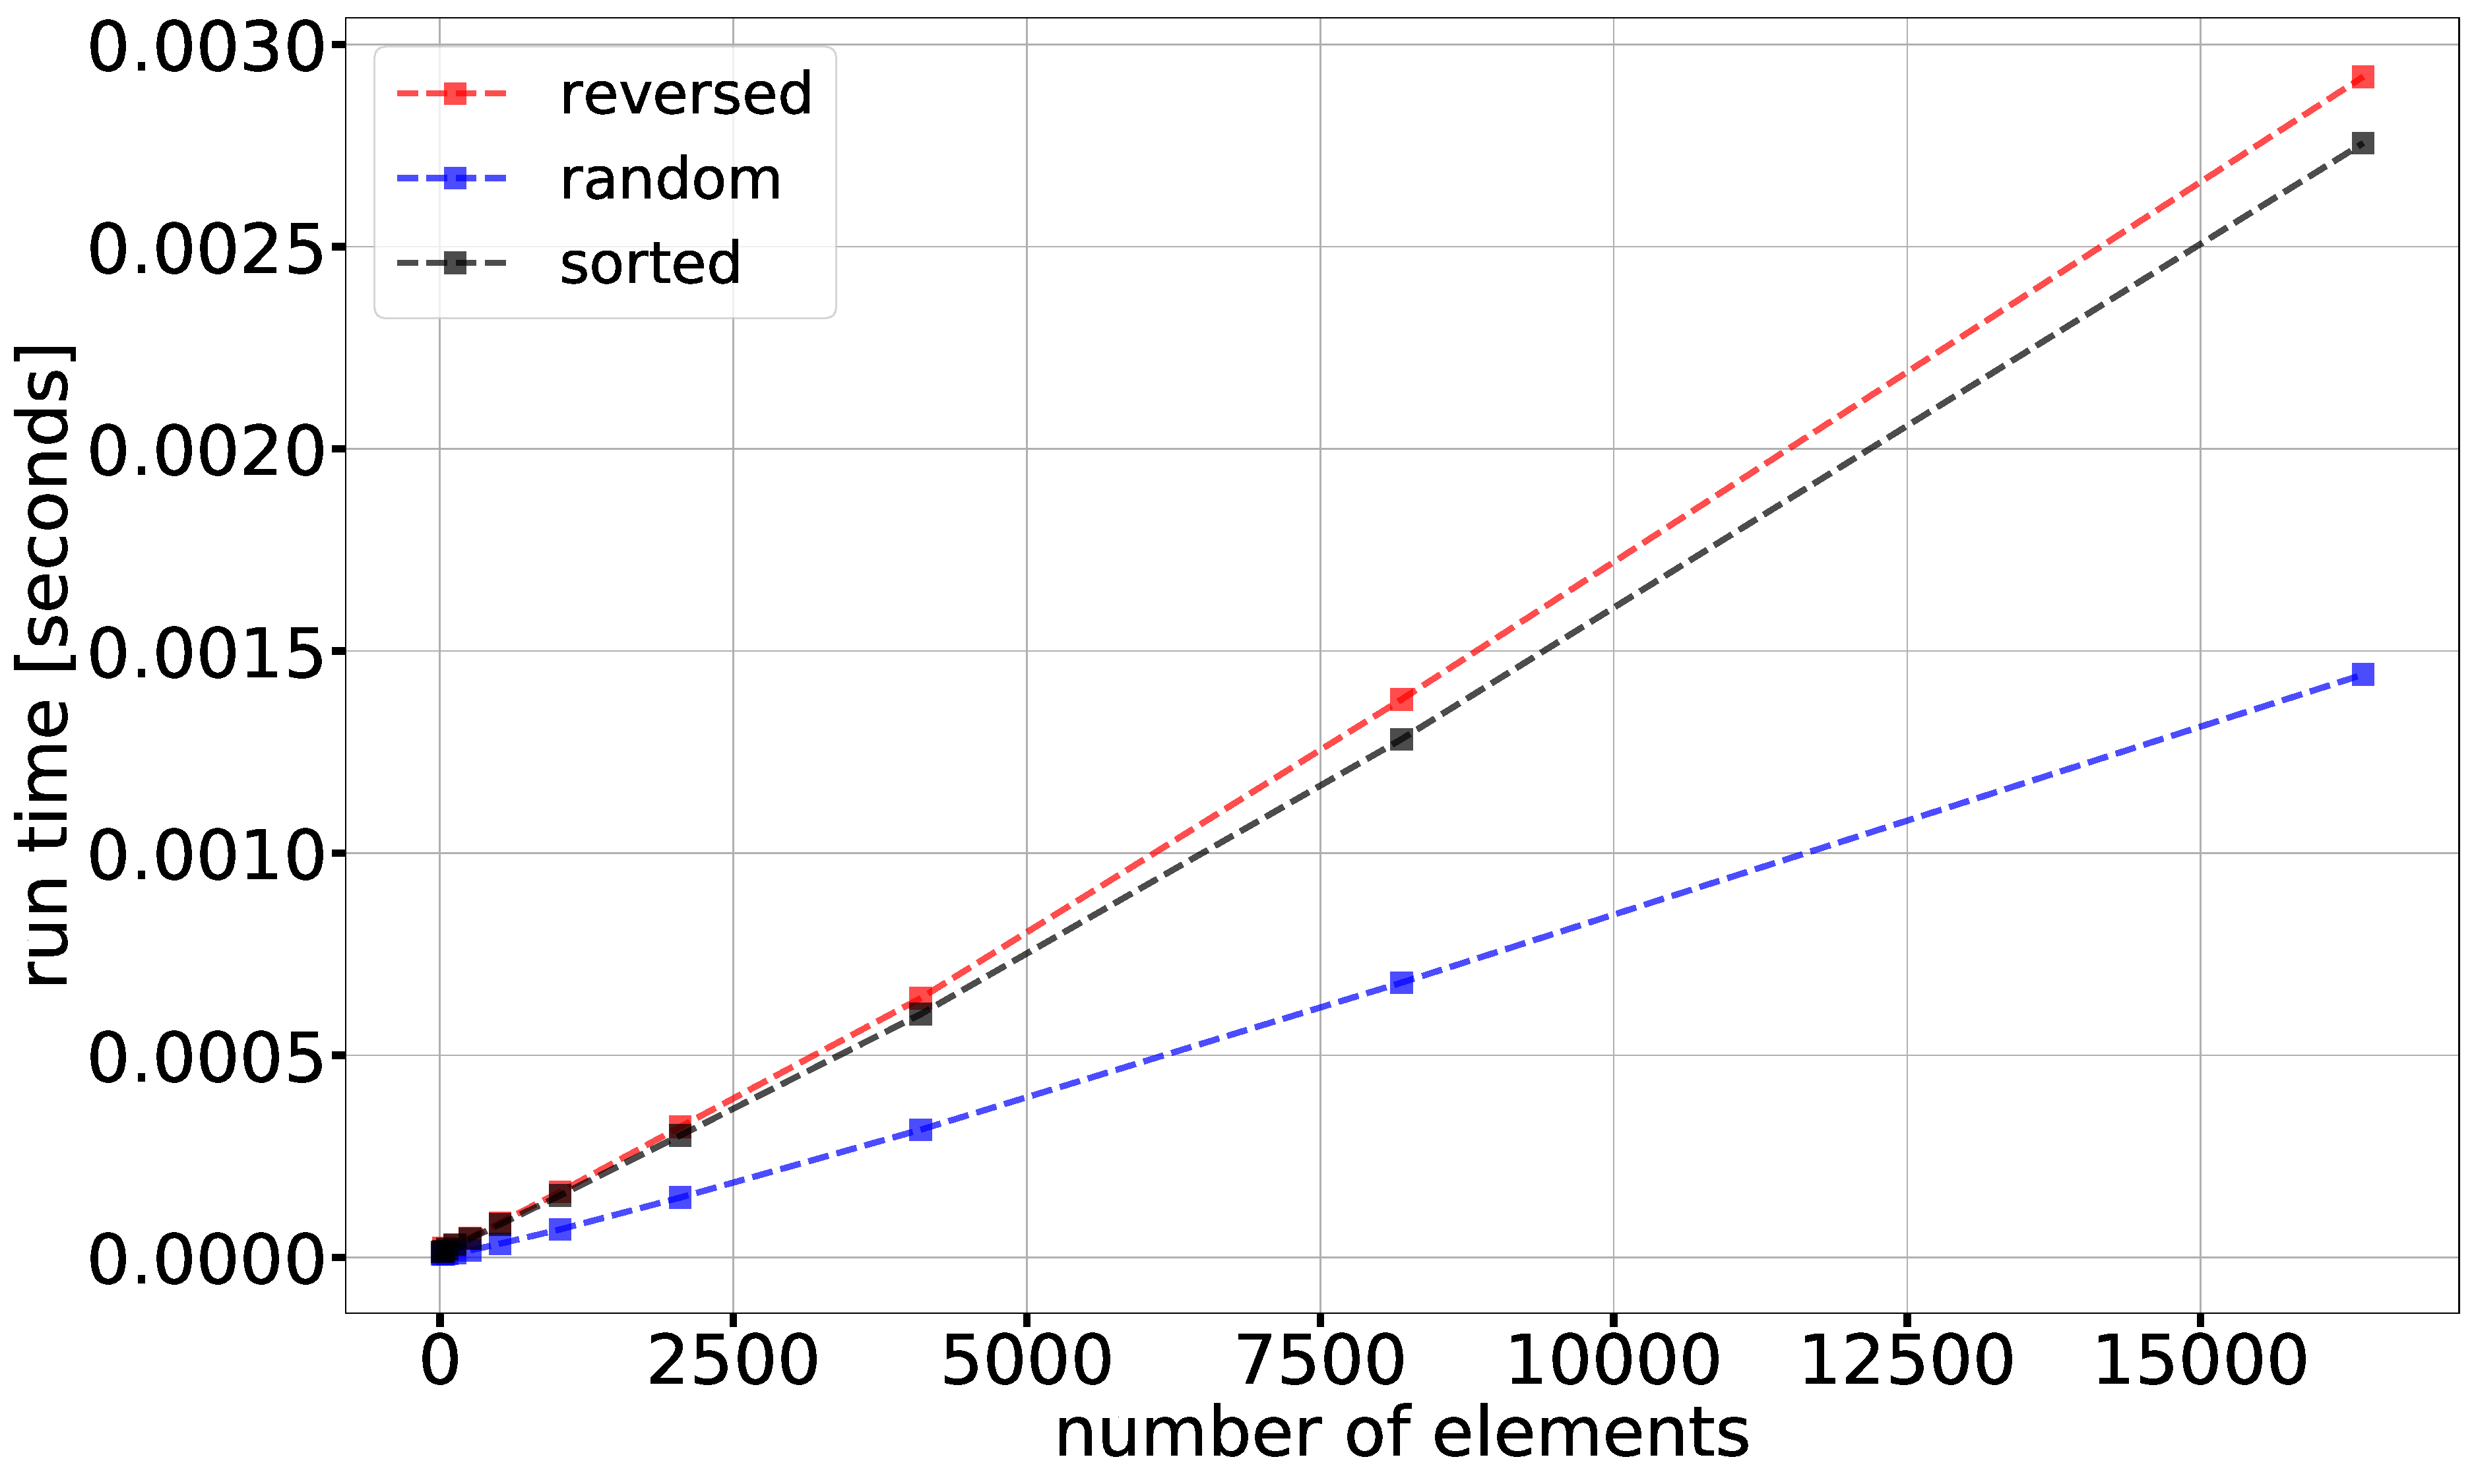
\includegraphics[width=84mm]{../figures/np_sort.pdf}
  % figure captions below figure
  \caption{Benchmark results for Numpy-Sort}
  \label{fig:np}
\end{figure}

\subsection{Number of Comparisons}\label{sec:nr_comparisons}
For further analysis of the observations of Merge-Sort and Quick-Sort algorithms, we used a counter to measure number of executed comparisons by the algorithms using the different data permutations. Figure~\ref{fig:comparisons} shows the recorded number of comparisons. Merge-Sort and Quick-Sort have the exact same number of comparisons when sorting reversed and sorted data. The number of comparisons differs in the case of random data. Taking an example of a list with the size $1024$, Merge-Sort execute $21503$ comparisons to sort the sorted or the reversed data. On the other hand, it executes $22289$ comparisons to sort the random data. For Quick-Sort, it executes $8716$ comparisons to sort the reversed data or the sorted data while it executes $11682$ comparisons to sort the random data.

\begin{figure}
  \centering
  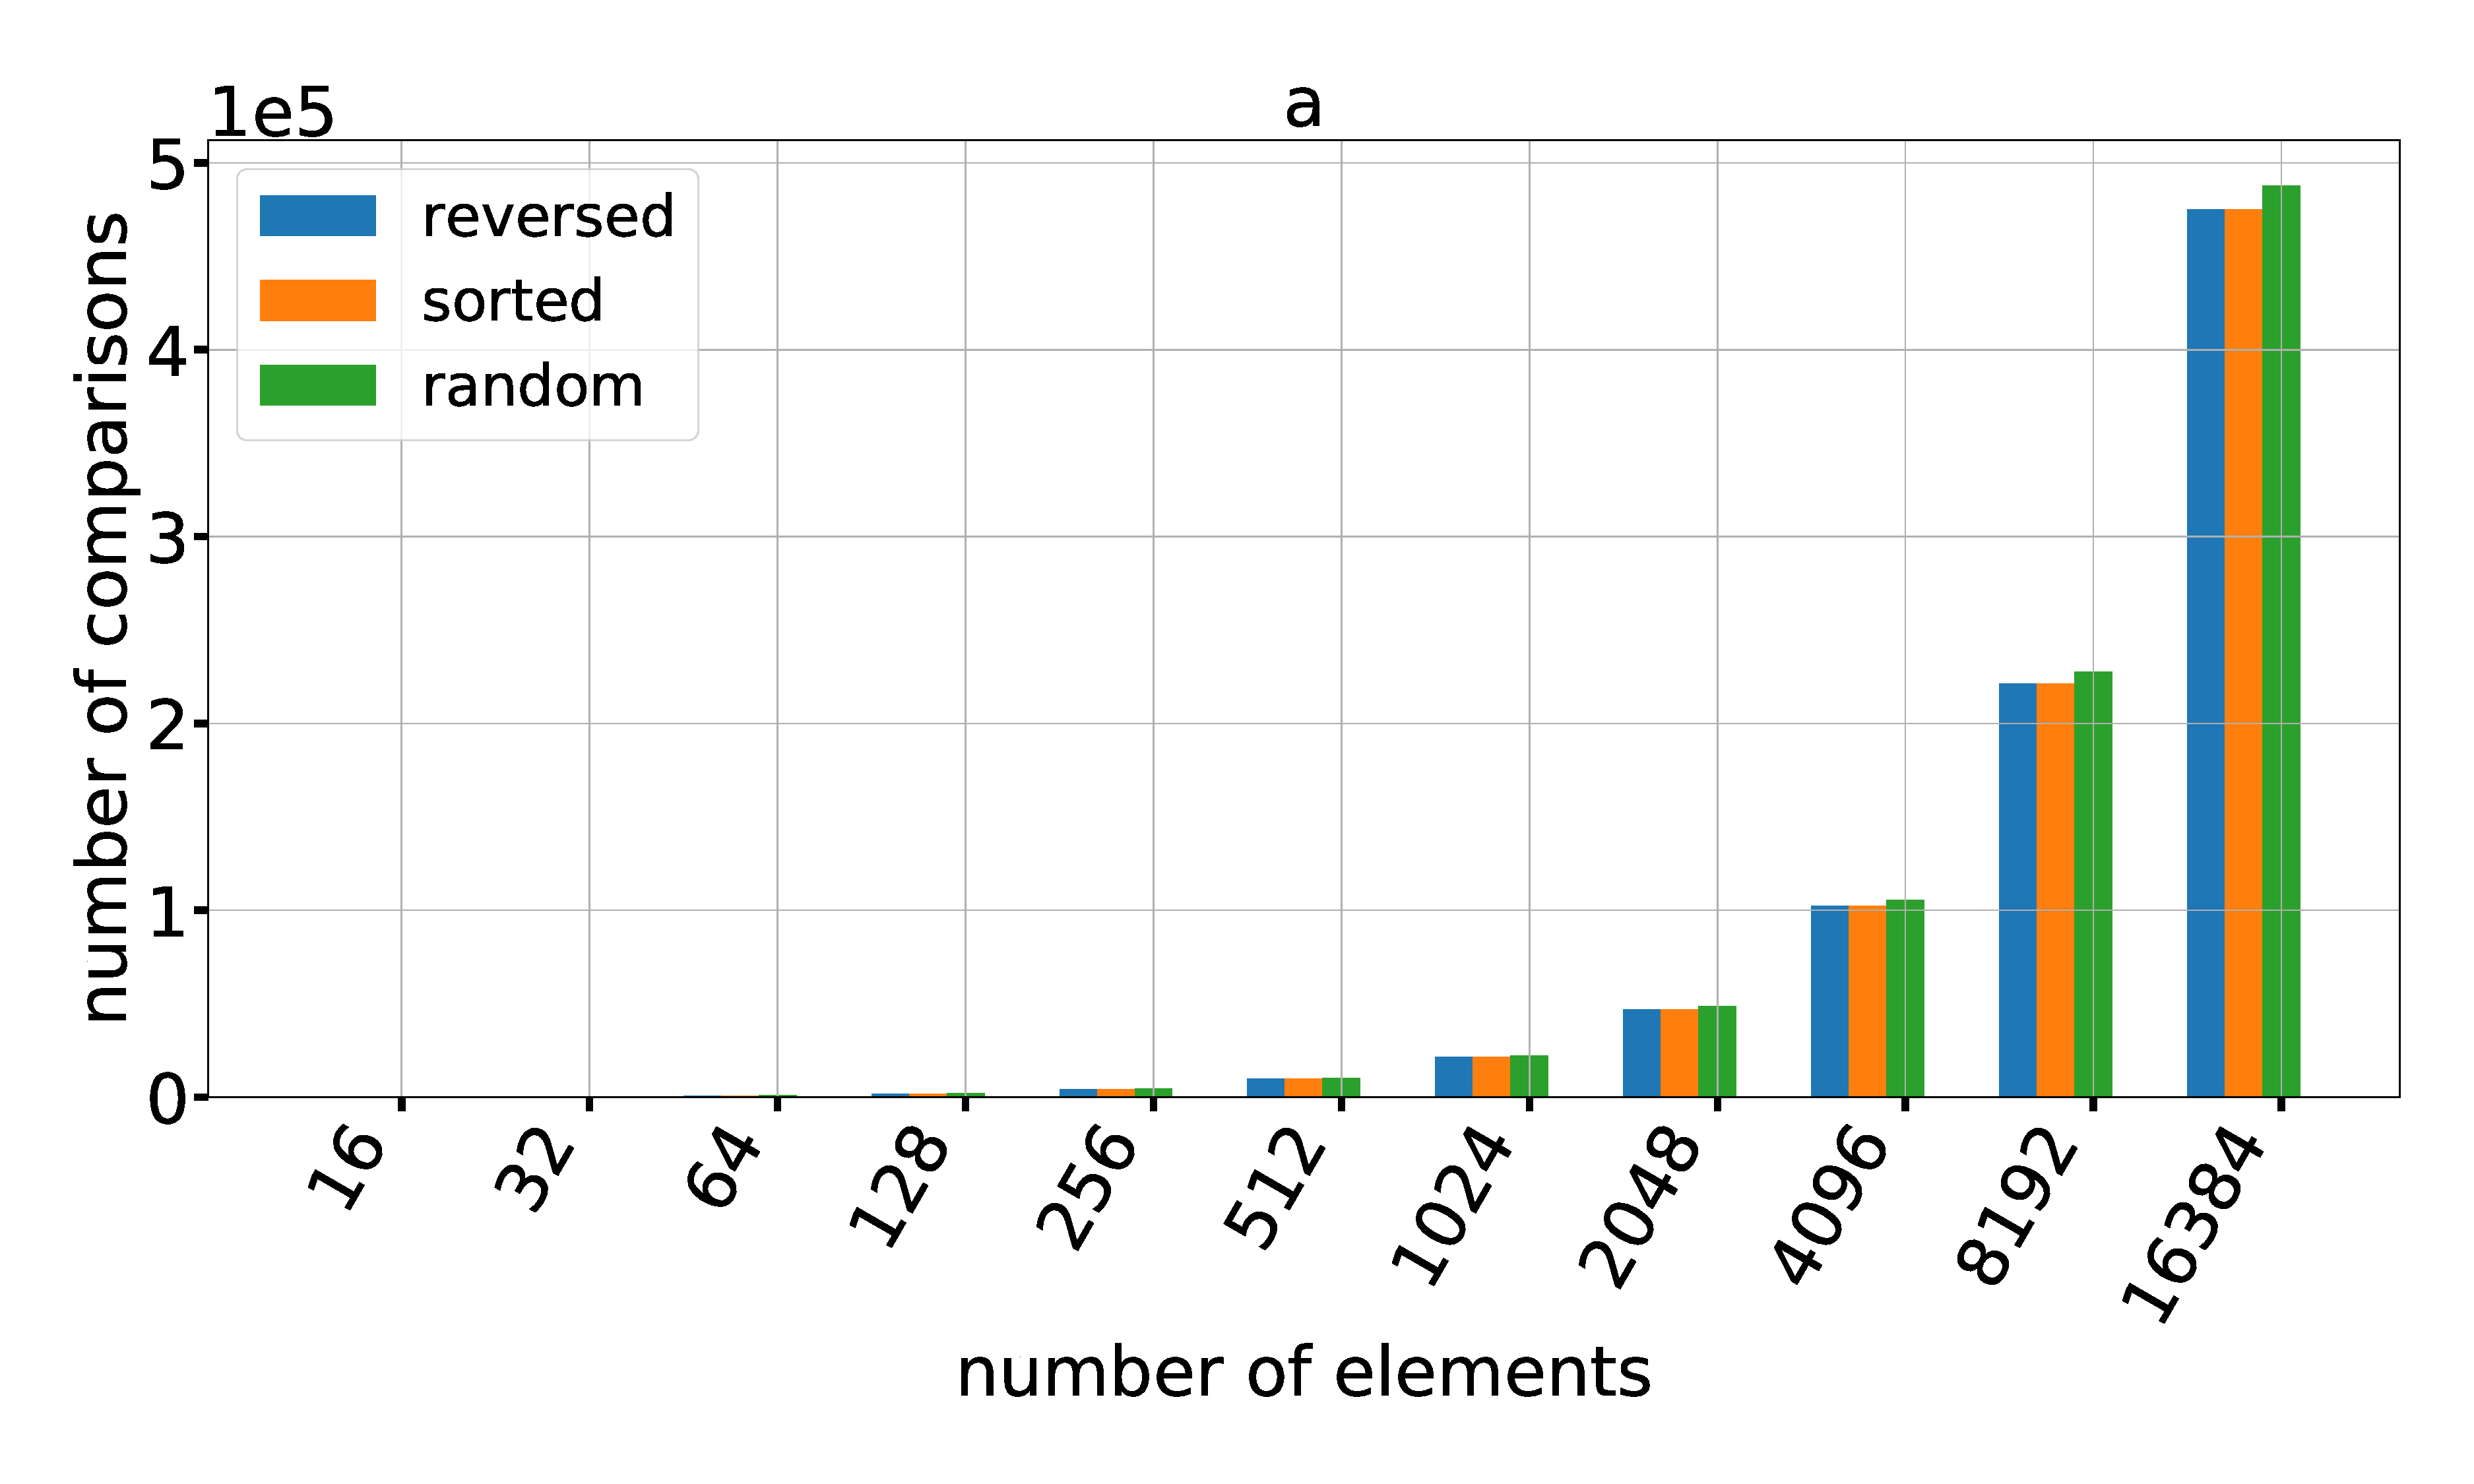
\includegraphics[width=84mm]{../figures/merge_number_comparisons.pdf}
  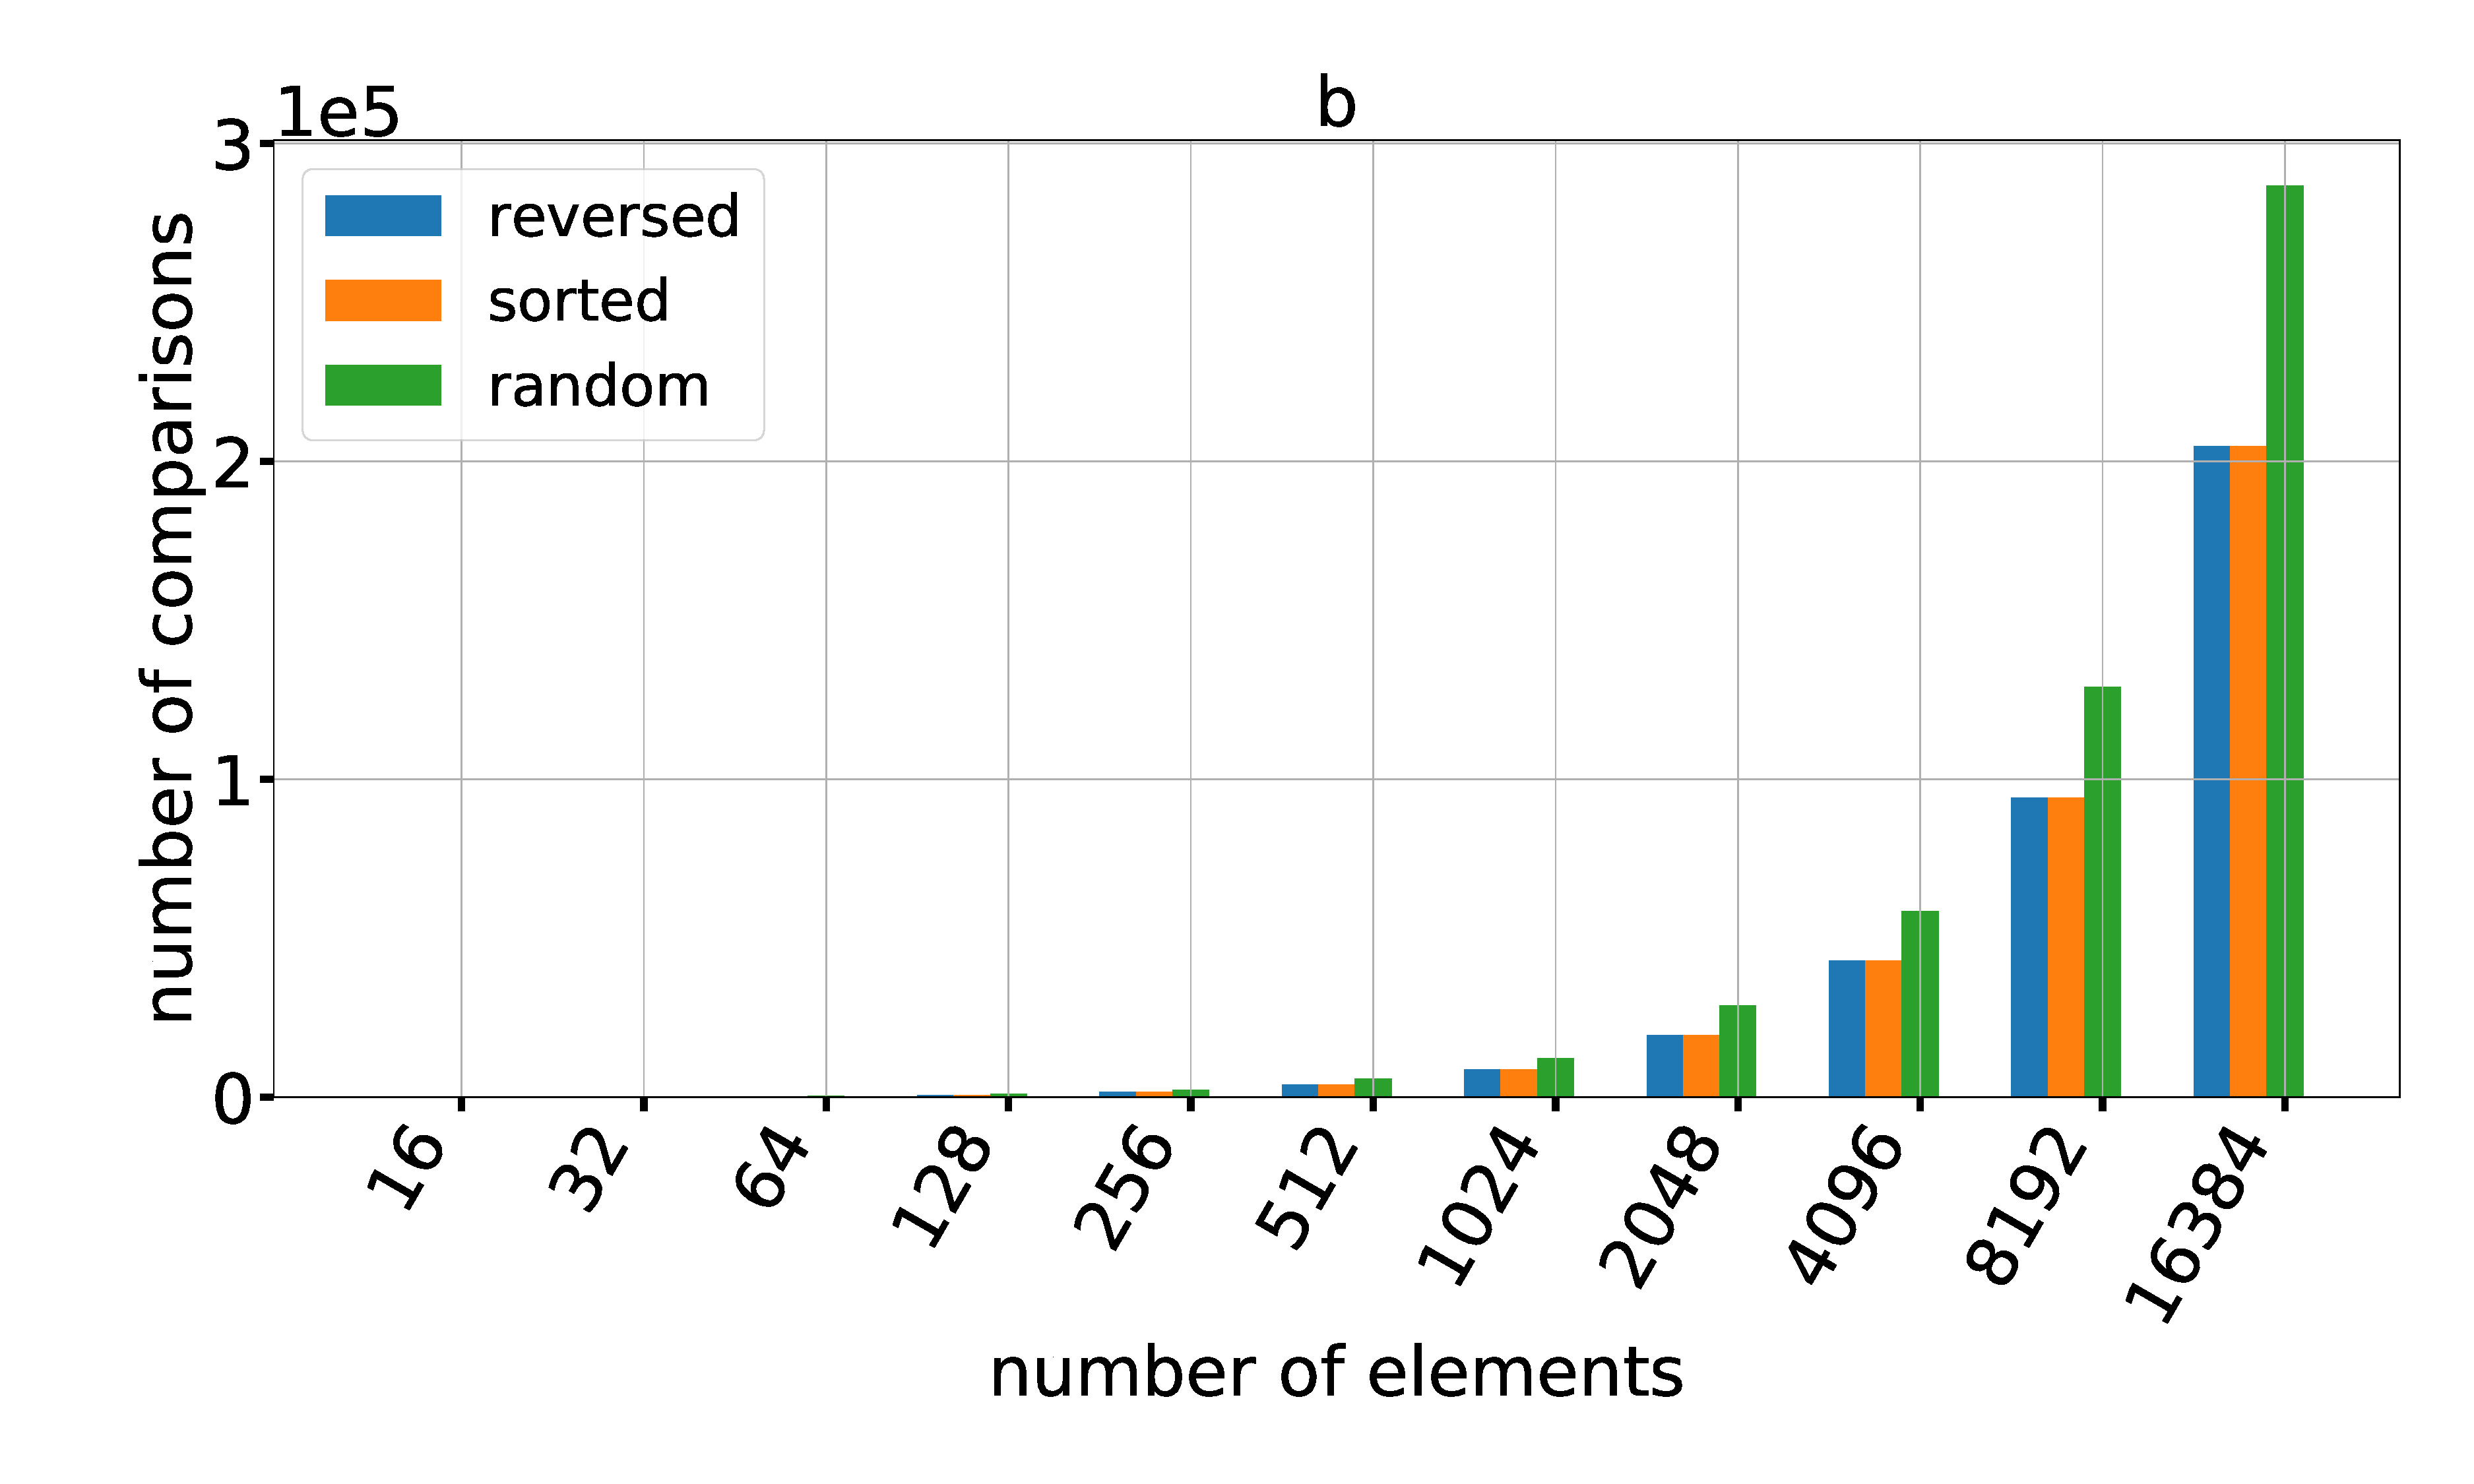
\includegraphics[width=84mm]{../figures/quick_number_comparisons.pdf}
  % figure captions below figure
  \caption{Number of comparisons for a)Merge-Sort and b)Quick-Sort using different data permutations and different data sizes}
  \label{fig:comparisons}
\end{figure}



\section{Discussion}\label{sec:discu}
\subsection{Quadratic Sorts}\label{sec:quad-disc}
Both Bubble-Sort and Insertion-Sort proved to follow quadratic run-time in general except the case of using Insertion-Sort on sorted data which followed a linear run-time. Theoretically, the worst case scenario for Bubble-Sort and Insertion-Sort happens when the used data is in reversed order. The recorded run-time showed that it did not follow the theory as sorting random data was worse than sorting reversed data. Insertion-Sort proved to be $4$ times faster than Bubble-Sort using the random data. Also, Insertion-Sort shows that it is more than $2$ times faster than Bubble-Sort on sorting reversed data which follows the results measured by \citet{astrachan}. 

\subsection{Sub-Quadratic Sorts}\label{sec:sub-quad-disc}
Asymptotically, Merge-Sort and Quick-Sort always take $\Theta(n \cdot \lg n)$ time ignoring the worst case of Quick-Sort. But we argue here that the cases which require more comparisons would take more time. So, if different list permutations have the same number of comparisons, that would lead to a similar run-time. Merge-Sort showed similar run-time for sorting sorted and reversed data which was attributed to the implemented algorithm in listing~\ref{lst:merge_sort} that executed the same number of comparisons in sorting sorted and reversed data. Performance got worse on sorting the random data as the number of comparisons increased as shown in figure~\ref{fig:comparisons}. Similarly, Quick-Sort showed similar results from sorted and reversed data because the number of comparisons were identical for sorted and reversed data. Quick-Sort is $2$ to $3$ times faster than Merge-Sort and these observations support the claims made by \citet{skienna08}. 

\subsection{Merge-Insertion-Sort}\label{sec:comb-disc}
The combined Merge-Insertion-Sort did not have a dramatic change in performance in comparison with Merge-Sort as explained in details in the results section. The slight improvement in performance on sorting the already sorted data is attributed to the introduction of the Binary-Insertion-Sort. Binary-Insertion-Sort follows a linear function to sort sorted data. Additionally, the decrease in performance on sorting reversed ordered data was because Binary-Insertion-Sort follows a quadratic run-time in sorting reversed ordered data.           

\subsection{Built-in Sorts}\label{sec:builtin-disc}
Since Python-Sort uses Tim-Sort, we expected that the run-time for sorting the already sorted data and reversed data should not be similar and the results did not follow this argument. That is because our implementation of Tim-Sort is still not the same as the \citet{cpythonsourcecode} implementation of Tim-Sort. This introduced a challenge to study the \citet{cpythonsourcecode} implementation of Tim-Sort in details to understand what made it $10$ times faster than our implementation of Merge-Insertion-Sort. Further work in this area is needed to give an explanation of the performance of Python-Sort. 
Numpy-Sort also followed the same phenomena of Quick-Sort where the run-time of sorting reversed or sorted data is relatively similar. That is because Numpy-Sort uses Quick-Sort by default. For data length $16384$, the run-times were $0.002756$ and $0.002920$ seconds for sorting the already sorted and reversed data respectively. This is because the algorithm is using Quick-Sort that has identical number of comparisons for sorting sorted and reversed data. However, using Numpy-Sort to sort random data was $2$ times faster than using Numpy-Sort to sort the already sorted data. This observation differed from the observation of Quick-Sort. This introduced another challenge to study \citet{harris2020array} implementation of Numpy-Sort in details.

\section{Conclusion}\label{sec:conclusion}
In this study, we implemented benchmark testing on several sorting algorithms using several input data permutations. Bubble-Sort and Insertion-Sort proved to follow quadratic run-time. Insertion-Sort proved best case scenario on sorted data as it was expected. Also, Insertion-Sort proved to be more efficient than Bubble-Sort which supported \citet{astrachan} claims. \newline
Quick-Sort and Merge-Sort shared an interesting phenomena that they showed the same run-time for sorting the already sorted and reversed sorted data which was analysed further by studying the number of executed comparisons. Quick-Sort was $2$ times faster than Merge-Sort which supported the claims of \citet{skienna08}. Combined Merge-Insertion-Sort gave slightly better results than Merge-Sort but it was still inferior to Quick-Sort. \newline
Python-Sort uses Merge-Sort at larger data which means the execution time should be similar for sorting the already sorted and reversed sorted data which is recorded in the results. Sorting random data was recorded to have poorer performance than sorting the already sorted and reversed data which follows Merge-Sort. Python-Sort showed that it is $10$ times faster than our implementation of Tim-Sort. Numpy-Sort showed interesting results that was not as predicted where it showed that Numpy-Sort is $2$ times faster when sorting random data than sorting sorted or reversed data. Further work is needed to understand the performance of the \citet{cpythonsourcecode} implementation of Tim-Sort and \citet{harris2020array} implementation of Numpy-Sort in details.


% In the acks section, you can thank people for help.
\begin{acks}
We want to express our gratitude to Prof. Hans Plesser for the guidance through this study. We would also like to thank PhD candidate Bao Ngoc Huynh for her suggestions and comments.
\end{acks}


%% The next two lines define the bibliography style to be used, and
%% the bibliography file.
\bibliographystyle{ACM-Reference-Format}
\bibliography{biblio_file}

\end{document}
